%!TeX TS-program = pdflatex
%!TeX encoding = UTF-8 Unicode
%!TeX spellcheck = en-US
%!BIB TS-program = bibtex
% -*- coding: UTF-8; -*-
% vim: set fenc=utf-8
% R0 https://www.biorxiv.org/content/10.1101/784116v1.full.pdf
% TODO R1 sur biorxiv
%: %%%%%%%%%%%%%%%%%%%%%%%%%%%%%%%%%%%%%%%%%%%%%%%%%%%%%%%%%%%%%%%%%%%%
\newcommand{\AuthorA}{Chlo\'e Pasturel}
\newcommand{\AuthorB}{Anna Montagnini}%
\newcommand{\AuthorC}{Laurent Perrinet}%
\newcommand{\Address}{Institut de Neurosciences de la Timone (UMR 7289), Aix Marseille Univ, CNRS - Marseille, France}%
\newcommand{\Website}{https://laurentperrinet.github.io}%
\newcommand{\EmailC}{Laurent.Perrinet@univ-amu.fr}%
\newcommand{\Title}{
Humans adapt their anticipatory eye movements to the volatility of visual motion properties
}
\newcommand{\Acknowledgments}{This work was supported by EU Marie-Sk\l{}odowska-Curie Grant No 642961 (PACE-ITN) and by the Fondation pour le Recherche M\'edicale, under the program \textit{Equipe FRM} (DEQ20180339203/PredictEye/G Masson). Code and material on the \href{\Website/publication/pasturel-montagnini-perrinet-20}{corresponding author's website}. We thank Doctor Jean-Bernard Damasse, Guillaume S Masson and Professor Laurent Madelain for insightful discussions. }
\newcommand{\KeyWords}{eye movements; decision making; volatility; Bayesian model; adaptation; perception}
%%%%%%%%%%%%%%%%%%%%%%%%%%%%%%%%%%%%%%%%%%
\documentclass[10pt,letterpaper]{article}
\usepackage[top=0.85in,left=2.75in,footskip=0.75in]{geometry}
\usepackage{amsmath,amssymb}
% Use adjustwidth environment to exceed column width (see example table in text)
\usepackage{changepage}
% Use Unicode characters when possible
\usepackage[utf8x]{inputenc}
% textcomp package and marvosym package for additional characters
\usepackage{textcomp,marvosym}
% cite package, to clean up citations in the main text. Do not remove.
\usepackage{cite}
% Use nameref to cite supporting information files (see Supporting Information section for more info)
\usepackage{nameref}
% line numbers
\usepackage[right]{lineno}
% ligatures disabled
\usepackage{microtype}
\DisableLigatures[f]{encoding = *, family = * }
% color can be used to apply background shading to table cells only
\usepackage[table]{xcolor}
% array package and thick rules for tables
\usepackage{array}
% create "+" rule type for thick vertical lines
\newcolumntype{+}{!{\vrule width 2pt}}
% create \thickcline for thick horizontal lines of variable length
\newlength\savedwidth
\newcommand\thickcline[1]{%
  \noalign{\global\savedwidth\arrayrulewidth\global\arrayrulewidth 2pt}%
  \cline{#1}%
  \noalign{\vskip\arrayrulewidth}%
  \noalign{\global\arrayrulewidth\savedwidth}%
}
% \thickhline command for thick horizontal lines that span the table
\newcommand\thickhline{\noalign{\global\savedwidth\arrayrulewidth\global\arrayrulewidth 2pt}%
\hline
\noalign{\global\arrayrulewidth\savedwidth}}
% Remove comment for double spacing
%\usepackage{setspace}
%\doublespacing
% Text layout
\raggedright
\setlength{\parindent}{0.5cm}
\textwidth 5.25in
\textheight 8.75in
% Bold the 'Figure #' in the caption and separate it from the title/caption with a period
% Captions will be left justified
\usepackage[aboveskip=1pt,labelfont=bf,labelsep=period,justification=raggedright,singlelinecheck=off]{caption}
\renewcommand{\figurename}{Fig}
% Use the PLoS provided BiBTeX style
\bibliographystyle{plos2015}
% Remove brackets from numbering in List of References
\makeatletter
\renewcommand{\@biblabel}[1]{\quad#1.}
\makeatother
% Header and Footer with logo
\usepackage{lastpage,fancyhdr,graphicx}
\usepackage{epstopdf}
%\pagestyle{myheadings}
\pagestyle{fancy}
\fancyhf{}
%\setlength{\headheight}{27.023pt}
%\lhead{\includegraphics[width=2.0in]{PLOS-submission.eps}}
\rfoot{\thepage/\pageref{LastPage}}
\renewcommand{\headrulewidth}{0pt}
\renewcommand{\footrule}{\hrule height 2pt \vspace{2mm}}
\fancyheadoffset[L]{2.25in}
\fancyfootoffset[L]{2.25in}
\lfoot{\today}
%% END MACROS SECTION
\newcommand{\KL}[2]{\text{KL}( #1 | #2 )}
%% parenthesis
\newcommand{\pa}[1]{\left( #1 \right)}
\newcommand{\bpa}[1]{\big( #1 \big)}
\newcommand{\choice}[1]{ %
	\left\{ %
		\begin{array}{l} #1 \end{array} %
	\right. }
% ensembles
\newcommand{\ens}[1]{ \{ #1 \} }
\newcommand{\enscond}[2]{ \left\{ #1 \;;\; #2 \right\} }
% egal par définition
\newcommand{\eqdef}{\ensuremath{\stackrel{\mbox{\upshape\tiny def.}}{=}}}
\newcommand{\eqset}{\ensuremath{\stackrel{\mbox{\upshape\tiny set}}{=}}}
\newcommand{\eq}[1]{\begin{equation*}#1\end{equation*}}
\newcommand{\eql}[1]{\begin{equation}#1\end{equation}}
\newcommand{\eqs}[1]{\begin{align*}#1\end{align*}}
\newcommand{\eqa}[1]{\begin{align}#1\end{align}}

\DeclareMathOperator{\argmin}{argmin}
\DeclareMathOperator{\argmax}{argmax}
\newcommand{\uargmin}[1]{\underset{#1}{\argmin}\;}
\newcommand{\uargmax}[1]{\underset{#1}{\argmax}\;}
\newcommand{\umin}[1]{\underset{#1}{\min}\;}
\newcommand{\umax}[1]{\underset{#1}{\max}\;}
\newcommand{\usup}[1]{\underset{#1}{\sup}\;}
% for units
\usepackage{siunitx}%
\newcommand{\ms}{\si{\milli\second}}%

%% Symboles arrondis
\newcommand{\Aa}{\mathcal{A}}
\newcommand{\Bb}{\mathcal{B}}
\newcommand{\Cc}{\mathcal{C}}
\newcommand{\Dd}{\mathcal{D}}
\newcommand{\Ee}{\mathcal{E}}
\newcommand{\Ff}{\mathcal{F}}
\newcommand{\Gg}{\mathcal{G}}
\newcommand{\Hh}{\mathcal{H}}
\newcommand{\Ii}{\mathcal{I}}
\newcommand{\Jj}{\mathcal{J}}
\newcommand{\Kk}{\mathcal{K}}
\newcommand{\Ll}{\mathcal{L}}
\newcommand{\Mm}{\mathcal{M}}
\newcommand{\Nn}{\mathcal{N}}
\newcommand{\Oo}{\mathcal{O}}
\newcommand{\Pp}{\mathcal{P}}
\newcommand{\Qq}{\mathcal{Q}}
\newcommand{\Rr}{\mathcal{R}}
\newcommand{\Ss}{\mathcal{S}}
\newcommand{\Tt}{\mathcal{T}}
\newcommand{\Uu}{\mathcal{U}}
\newcommand{\Vv}{\mathcal{V}}
\newcommand{\Ww}{\mathcal{W}}
\newcommand{\Xx}{\mathcal{X}}
\newcommand{\Yy}{\mathcal{Y}}
\newcommand{\Zz}{\mathcal{Z}}
\usepackage{gensymb} % \degree
%% ========  polices de caracteres =============
\usepackage[T1]{fontenc}%
\usepackage{lmodern}%
\usepackage{t1enc}
\usepackage{ragged2e}
%============ graphics ===================
\usepackage{graphicx}%
\DeclareGraphicsExtensions{.pdf,.png,.jpg}%
\graphicspath{{./figures/}}%
%============ bibliography ===================
\newcommand{\citep}[1]{\cite{#1}}
\newcommand{\citet}[1]{\cite{#1}}
%%%%%%%%%%%%%%%%%%%%%%%%%%%%%%
%% OPTIONAL MACRO FILES
\usepackage{tikz}
\newcommand{\seeFig}[1]{Figure~\ref{fig:#1}}
\newcommand{\seeEq}[1]{Equation~\ref{eq:#1}}
\newcommand{\seeApp}[1]{Appendix~\ref{app:#1}}
\newcommand{\seeSec}[1]{Section~\ref{sec:#1}}
%============ hyperref ===================
\usepackage[unicode,linkcolor=red,citecolor=red,filecolor=red,urlcolor=red,pdfborder={0 0 0}]{hyperref}%
%\hypersetup{%
%pdftitle={\Title},%
%pdfauthor={\AuthorA }%\ < \Email > \Address},%
%}%
\usepackage{color}%
\newcommand{\LP}[1]{\textbf{\textcolor{red}{[LP: #1]}}}
\newcommand{\Rone}[1]{\textbf{\textcolor{magenta}{[rev 1: #1]}}}
\newcommand{\AM}[1]{\textbf{\textcolor{blue}{[AM: #1]}}}
\newcommand{\CP}[1]{\textbf{\textcolor{green}{[CP: #1]}}}
\usepackage{listings}
\definecolor{dkgreen}{rgb}{0,0.6,0}
\definecolor{gray}{rgb}{0.5,0.5,0.5}
\definecolor{mauve}{rgb}{0.58,0,0.82}
%============ code ===================
\usepackage{listings}
\lstset{frame=tb,
  language=Python,
  aboveskip=3mm,
  belowskip=3mm,
  showstringspaces=false,
  columns=flexible,
  basicstyle={\small\ttfamily},
  numbers=none,
  numberstyle=\tiny\color{gray},
  keywordstyle=\color{blue},
  commentstyle=\color{dkgreen},
  stringstyle=\color{mauve},
  breaklines=true,
  breakatwhitespace=true,
  tabsize=3
}
%%%%%%%%%%%%%%%%%%%%%%%%%%%%%%%%%%%
\title{\Title}%
\author{\AuthorA,
\AuthorB,
\AuthorC\thanks{\Address} }
\linenumbers
%%%%%%%%%%%% Her begynner selve dokumentet %%%%%%%%%%%%%%%
\begin{document}%
\maketitle%
%%%%%%%%%%%%%%%%%%%%%%%%%%%%%%%%%%%%%%%%%%%%%%%%%%%%%%%%%%%%%%%%
%: Abstract
\section*{Abstract}
Animal behavior constantly adapts to changes, for example when the statistical properties of the environment change unexpectedly. For an agent that interacts with this volatile setting, it is important to react accurately and as quickly as possible. It has already been shown that when a random sequence of motion ramps of a visual target is biased to one direction (e.g. right or left), human observers adapt their eye movements to accurately anticipate the target's expected direction. Here, we prove that this ability extends to a volatile environment where the probability bias could change at random switching times. In addition, we also recorded the explicit prediction of the next outcome as reported by observers using a rating scale. Both results were compared to the estimates of a probabilistic agent that is optimal in relation to the assumed generative model. Compared to the classical leaky integrator model, we found a better match between our probabilistic agent and the behavioral responses, both for the anticipatory eye movements and the explicit task. Furthermore, by controlling the level of preference between exploitation and exploration in the model, we were able to fit for each individual's experimental dataset the most likely level of volatility and analyze inter-individual variability across participants. These results prove that in such an unstable environment, human observers can still represent an internal belief about the environmental contingencies, and use this representation both for sensory-motor control and for explicit judgments. This work offers an innovative approach to more generically test the diversity of human cognitive abilities in uncertain and dynamic environments.
% Please keep the Author Summary between 150 and 200 words
% Use first person. PLOS ONE authors please skip this step.
% Author Summary not valid for PLOS ONE submissions.
\section*{Author summary}
Understanding how humans adapt to changing environments to make judgments or plan motor responses based on time-varying sensory information is crucial for psychology, neuroscience and artificial intelligence. Current theories for how we deal with the environment's uncertainty, that is, in response to the introduction of some randomness change, mostly rely on the behavior at equilibrium, long after after a change. Here, we show that in the more ecological case where the context switches at random times all along the experiment, an adaptation to this volatility can be performed online. In particular, we show in two behavioral experiments that humans can adapt to such volatility at the early sensorimotor level, through their anticipatory eye movements, but also at a higher cognitive level, through explicit ratings. Our results suggest that humans (and future artificial systems) can use much richer adaptive strategies than previously assumed.
%: %%%%%%%%%%%%%%%%%%%%%%%%%%%%%%%%%%%%%%%%%%%%%%%%%%%%%%%%%%%%%%%
\section{Motivation}
%%%%%%%%%%%%%%%%%%%%%%%%%%%%%%%%%%%%%%%%%%%%%%%%%%%%%%%%%%%%%%%%
\label{sec:intro}
%%%%%%%%%%%%%%%%%%%%%%%%%%%%%%%%%%%%%%%%%%%%%%%%%%%%%%%%%%%%%%%%
%%%%%%%%%%%%%%%%%%%%%%%%%%%%%%%%%%%%%%%%%%%%%%%%%%%%%%%%%%%%%%%%
\subsection{Volatility of sensory contingencies and the adaptation of cognitive systems}
%: 1A : cognitive adaptation to volatility; general volatility and perceptual learning
%-------------------------------------------------------------%
% ------------------------------------------------------------------
We live in a fundamentally volatile world for which
our cognitive system has to constantly adapt.
In particular, this volatility may be generated
by processes with different time scales.
Imagine for instance you are a general practitioner and
that you usually report an average number of
three persons infected by flu per week.
However, this rate is variable and
over the past week you observe that the rate increased to ten cases.
In consequence, two alternative interpretations are available:
the first possibility is that there is an outbreak of flu and
one should then estimate its incidence
(i.e. the rate of new cases)
since the inferred outbreak's onset, in order
to quantify the infection rate specific to this outbreak,
but also to update the value of %the environmental volatility (as given by
the probability of a new outbreak %)
at a longer time scale.
Alternatively, these cases are
``unlucky'' coincidences that originate from the natural variability
of the underlying statistical process which drive patients to the doctor,
and which are instances drawn from the same stationary random process.
In that option, it may be possible to readjust
the estimated baseline rate of infection with this new data.
This example illustrates one fundamental problem
with which our cognitive system is faced:
when observing new sensory evidence,
\emph{should I stay} and continue to exploit this novel data
with respect to my current beliefs about the environment's state
or \emph{should I go} and explore a new hypothesis
about the random process generating the observations
since the detection of a switch in the environment?

This uncertainty in the environment's state is characterized by its \emph{volatility}
which by definition measures the temporal variability
of the sufficient parameters of a random variable.
Such meta-analysis of the environment's statistical properties
is an effective strategy at a large temporal scale level,
% \Rone{lines 61-63 the link to the flu outbreak could be made explicit.}\LP{Done... right?}
as that for the flu outbreak of our example,
but also at all levels which are behaviorally relevant,
such as contextual changes in our everyday life.
Inferring near-future states in a dynamic environment,
such that one can prepare to act upon them
ahead of their occurrence ---
or at least forming beliefs as precise as possible
about a future environmental context ---
is an ubiquitous challenge for cognitive systems~\citep{Barack16}.
In the long term, how the human brain dynamically manages
this trade-off between exploitation and exploration
is essential to the adaptation
of the behavior through reinforcement learning~\citep{Cohen2007}.

%: Past history of sensory event integration in vision
In controlled psychophysical experimental settings which challenge visual perception or sensorimotor associations,
such adaptive processes have been mostly put in evidence
by precisely analyzing the participants' behavior in a sequence of experimental trials.
These typically highlight sequential effects
at the time scale of several seconds to minutes
or even hours in the case of the adaptation to a persistent sensorimotor relation.
% \Rone{Paragraph 76-91 is rather obscure to me, it requires some more explanation. The link to adaptation and priming is probably misleading as the measure corresponds rather to a prediction of what happens next, those two effects are typically tested differently (a reduction of sensitivity and an increase in sensitivity)}
Indeed, stimulus history of sensory events influences
how the current stimulus is perceived~\citep{Sotiropoulos2011,Adams12,ChopinMamassian2012,FischerWhitney2014,Cicchini_PRSB_2018} and
acted upon~\citep{WallmanFuchs1998,Carpenter1995, Maus2015,Damasse18}.
Two qualitatively opposite effects of the stimulus history have been described:
negative (adaptation), and positive (priming-like) effects.
% \Rone{line 82: not clear how adaptation "favors spatial stability of the stimulus"}
Adaptation reduces the sensitivity to recurrently presented stimuli,
thus yielding a re-calibrated perceptual experience~\citep{Clifford2007, Webster2011, Kohn2007}.
%\AM{I WOULD DELETE Examples of negative biases in perceptual discrimination are numerous
%(see for instance~\citep{KanaiVerstraten2005,ChopinMamassian2012}) and
%show that the visual system tends
%to favor the temporal stability of the stimulus.}
On the other hand, priming is a facilitatory effect that
enhances the identification of repeated stimuli~\citep{Verstraten1994, Tiest2009}:
%\AM{I WOULD SKIP THIS This type of perceptual learning leads to improvements %in discrimination
%with long-term training on a perceptual judgment~\citep{Lu2009}.}
in sensorimotor control,
the same stimulus presented several times could indeed
lead to faster and more precise responses.
%\AM{I WOULD DELETE and,
%% \Rone{line 86: quite obscure}
%at the same time, lead to a suboptimal behavior
%as the enviroment changes and the presented stimulus is this time not coherent
%with the participant's expectations~\citep{Hyman1953, Yu2009}.
%This process is highly dynamic especially in complex environments
%where new contingencies can arise at every moment.}
Interestingly, priming effects %at cognitive levels
are sometimes paralleled by anticipatory motor responses
which are positively correlated with the repetition of stimulus properties.
A well-known example of this behavior
are anticipatory smooth eye movements (aSPEM or shortly, anticipatory pursuit),
as we will illustrate in the next section.

%: Bayesian methods & role of predictive processing for this adaptive response
Overall, the ability to take into account
statistical regularities in the event sequence appears as a fundamental ability
for the adaptive behavior of living species.
Importantly, few studies have addressed the question of whether
the estimate of such regularities is explicit,
and whether such explicit reports of the dynamic statistical
estimates would eventually correlate with the measures of behavioral adaptation or priming.
Here we aim at investigating this question
in the specific case of the  processing of a target's motion direction.
In addition, we attempt to palliate the lack of a solid modeling approach
to best understand the computation underlying behavioral adaptation to the environment's statistics,
and in particular how sequential effects are integrated
within a hierarchical statistical framework.

Bayesian inference offers an effective methodology
to deal with this question.
Indeed, these methods allow to define and quantitatively assess
a range of hypotheses about the processing of possibly noisy information by some formal agents~\citep{Deneve1999, Diaconescu2014, Daunizeau10a}.
A key principle in the Bayesian inference approach is
to introduce so-called \emph{latent variables}
which explicitly represent different hypotheses by the agent and how these may predict experimental outcomes.
Each hypothesis defines different weights in the graph of probabilistic dependencies between variables
(for instance between the number of patients at a practitioner and the reality of a flu pandemic).
%In practice, a generative model is used to to define such graph and  is parameterized by structural variables
%(such as weights or non-linear gain functions)
%which are for instance tuned by past statistics extracted from observations.
Then, using the rules of probability calculus and knowing incoming measurements,
one can progressively update beliefs about the latent variables,
and eventually infer the hidden structure underlying the received inputs~\citep{Hoyer2003, Ma2014}.
For instance, using Bayes's rule, one can combine
the likelihood of observations given a given generative model and
the prior on these latent variables~\citep{Jaynes2014}
such that beliefs about latent variables
may be represented as probabilities.
Of particular interest for us is the possibility to
quantitatively represent in this kind of probabilistic model
the predictive and iterative nature of a sequence of events.
Indeed, once the belief about latent variables
is formed from the sensory input,
this belief can be used to update
the prior over future beliefs~\citep{Montagnini2007}.
In such models, the comparison between expectations and actual data leads to
continuous updates of the estimates of the latent variables,
but also of the validity of the model.
There are numerous examples of Bayesian approaches
applied to the study of the adaptation to volatility.
For instance, Meyniel et al~\citet{Meyniel16} simulated a hierarchical Bayesian model
over five previously published datasets~\citep{Squires1976, Huettel2002, Kolossa2013, Cho2002, Falk1997}
in the domain of cognitive neuroscience.
%\AM{NOT NECESSARY HERE Their main conclusion was that
%learning the local transition probabilities
%was sufficient to explain the large repertoire
%of experimental effects reported in all these studies.}
Here we focus on an extension of this approach to the study of motion processing and eye movements.
% ------------------------------------------------------------------
\subsection{Anticipatory Smooth Pursuit Eye Movements (aSPEM)}
% ------------------------------------------------------------------
%: 1B : particular case of anticipatory pursuit
%: adaptation to volatility in EMs : seen as an anticipation in SPEM - principle and function
Humans are able to accurately track a moving object
with a combination of saccades and
Smooth Pursuit Eye Movements (for a review see~\citet{Krauzlis2008}).
These movements allow us to align and
stabilize the object on the fovea,
thus enabling high-resolution visual processing.
This process is delayed by different factors such as axonal transduction,
neural processing latencies and the inertia of the oculomotor system~\citep{Krauzlis89}.
When predictive information is available about target's motion,
an anticipatory Smooth Pursuit Eye Movement (aSPEM or shortly, anticipatory pursuit)
is generated before its appearance~\citep{Westheimer1954, Kowler1979a, Kowler1979b}
thereby reducing visuomotor latency~\citep{PerrinetAdamasFriston2014}.
Moreover, some experiments have demonstrated the existence
of prediction-based smooth pursuit maintenance during
the transient disappearance of a moving target~\citep{Badler2006,BeckerFuchs1985,OrbandeXivryMissalLefevre_JOV2012}
and even predictive acceleration or deceleration during visual tracking~\citep{BeckerFuchs1985,CollinsBarnes2009}.
Overall, although the initiation of smooth pursuit eye movements
is almost always driven by a visual motion signal,
it is now clear that smooth pursuit behavior
can be modulated at different stages by extra-retinal, predictive information even in the absence of a direct visual stimulation~\citep{Barnes2008}.
Several functional and computational models have been proposed in the literature for the different forms of prediction-based smooth eye movements, such as zero-lag tracking of a periodic target~\citep{DallosJones1963} or pursuit maintenance during target occlusion~\citep{CollinsBarnes2009}. More recently an effort has been made to provide a more general theoretical framework, which is based on Bayesian inference and the reliability-based cue combination. Although the mapping of this theoretical framework onto neuronal functions remains to be elucidated, it has the clear advantage of generality, as for instance, it would encompass all forms of smooth pursuit behavior, including prediction-based and visually-guided tracking~\citep{Bogadhi2013,Orban2013,Deravet_JOV2018,Darlington_NatNeu2018}. Here, we present a model extending this recent theoretical effort to include the adaptivity to a volatile environment.

Experience-based anticipatory pursuit behavior is remarkable
in different aspects.
First, its buildup is relatively fast, such that only a few trials are sufficient
to observe the effects of specific regularities in the properties of visual motion, such as speed, timing or direction~\citep{Kowler1984,Maus2015,Deravet_JOV2018}.
Second, it is a robust phenomenon, which has been observed on a large population of human participants and even in non-human primates (for a recent review see~\citet{Kowler_AnnRev2019}). Note also, that human participants seem to be largely unaware of this behavior (as inferred from informal questioning). Finally, this kind of behavior has proven to be exquisitely sensitive to the probabilistic properties of the sensorimotor context.

%: linear relationship (talk about santos & kowler and others)
Typically, anticipatory pursuit is observed after a temporal cue and
before target motion onset~\citep{Kowler1979a,Kowler1979b, Kowler1984}. %~(see \seeFig{intro}-A).
In previous studies~\citep{Montagnini2010,Damasse18},
we have analyzed how forthcoming motion properties,
such as target speed or direction, can be anticipated with coherently oriented eye movements. %~(see \seeFig{intro}-A).
We have observed that the amplitude of anticipation,
as measured by the mean anticipatory eye velocity,
increases when the target repeatedly moves in the same direction.
In particular, the mean anticipatory eye velocity is linearly related
to the probability of motion's speed or direction. %~(see \seeFig{intro}-B).
These results are coherent with findings
by other groups~\citep{Kowler1984, Kowler1989, Heinen2005,SantosKowler2017} and
they indicate that anticipatory pursuit behavior is potentially a useful marker
to study the internal representation of motion expectancy, %(or Prior)
and in particular to analyze how such expectancy
is dynamically modulated by probabilistic contingencies in shaping oculomotor behavior.
%
%-------------------------------------------------------------%
%: FIGURE 1 fig:intro~\seeFig{intro}
\begin{figure}%[b!]
\centering{
\begin{tikzpicture}%[thick,scale=1, every node/.style={scale=1} ]
\node [anchor=north west] (imgA) at (0.000\linewidth,.600\linewidth){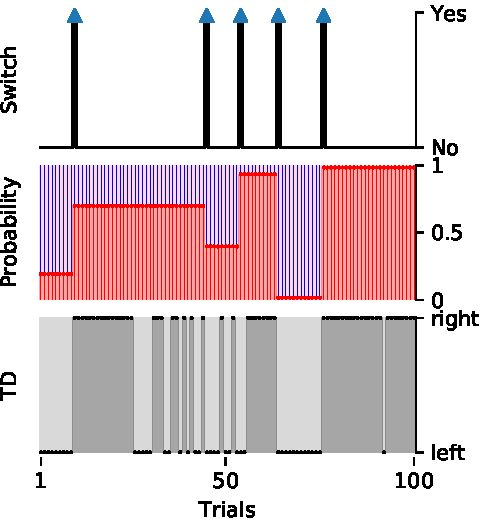
\includegraphics[width=0.325\linewidth]{1_A_Experiment_randomblock}};
\node [anchor=north west] (imgB) at (0.335\linewidth,.595\linewidth){\includegraphics[width=0.350\linewidth]{1_B_protocol_recording}};
\node [anchor=north west]  (imgC) at (0.650\linewidth,.595\linewidth){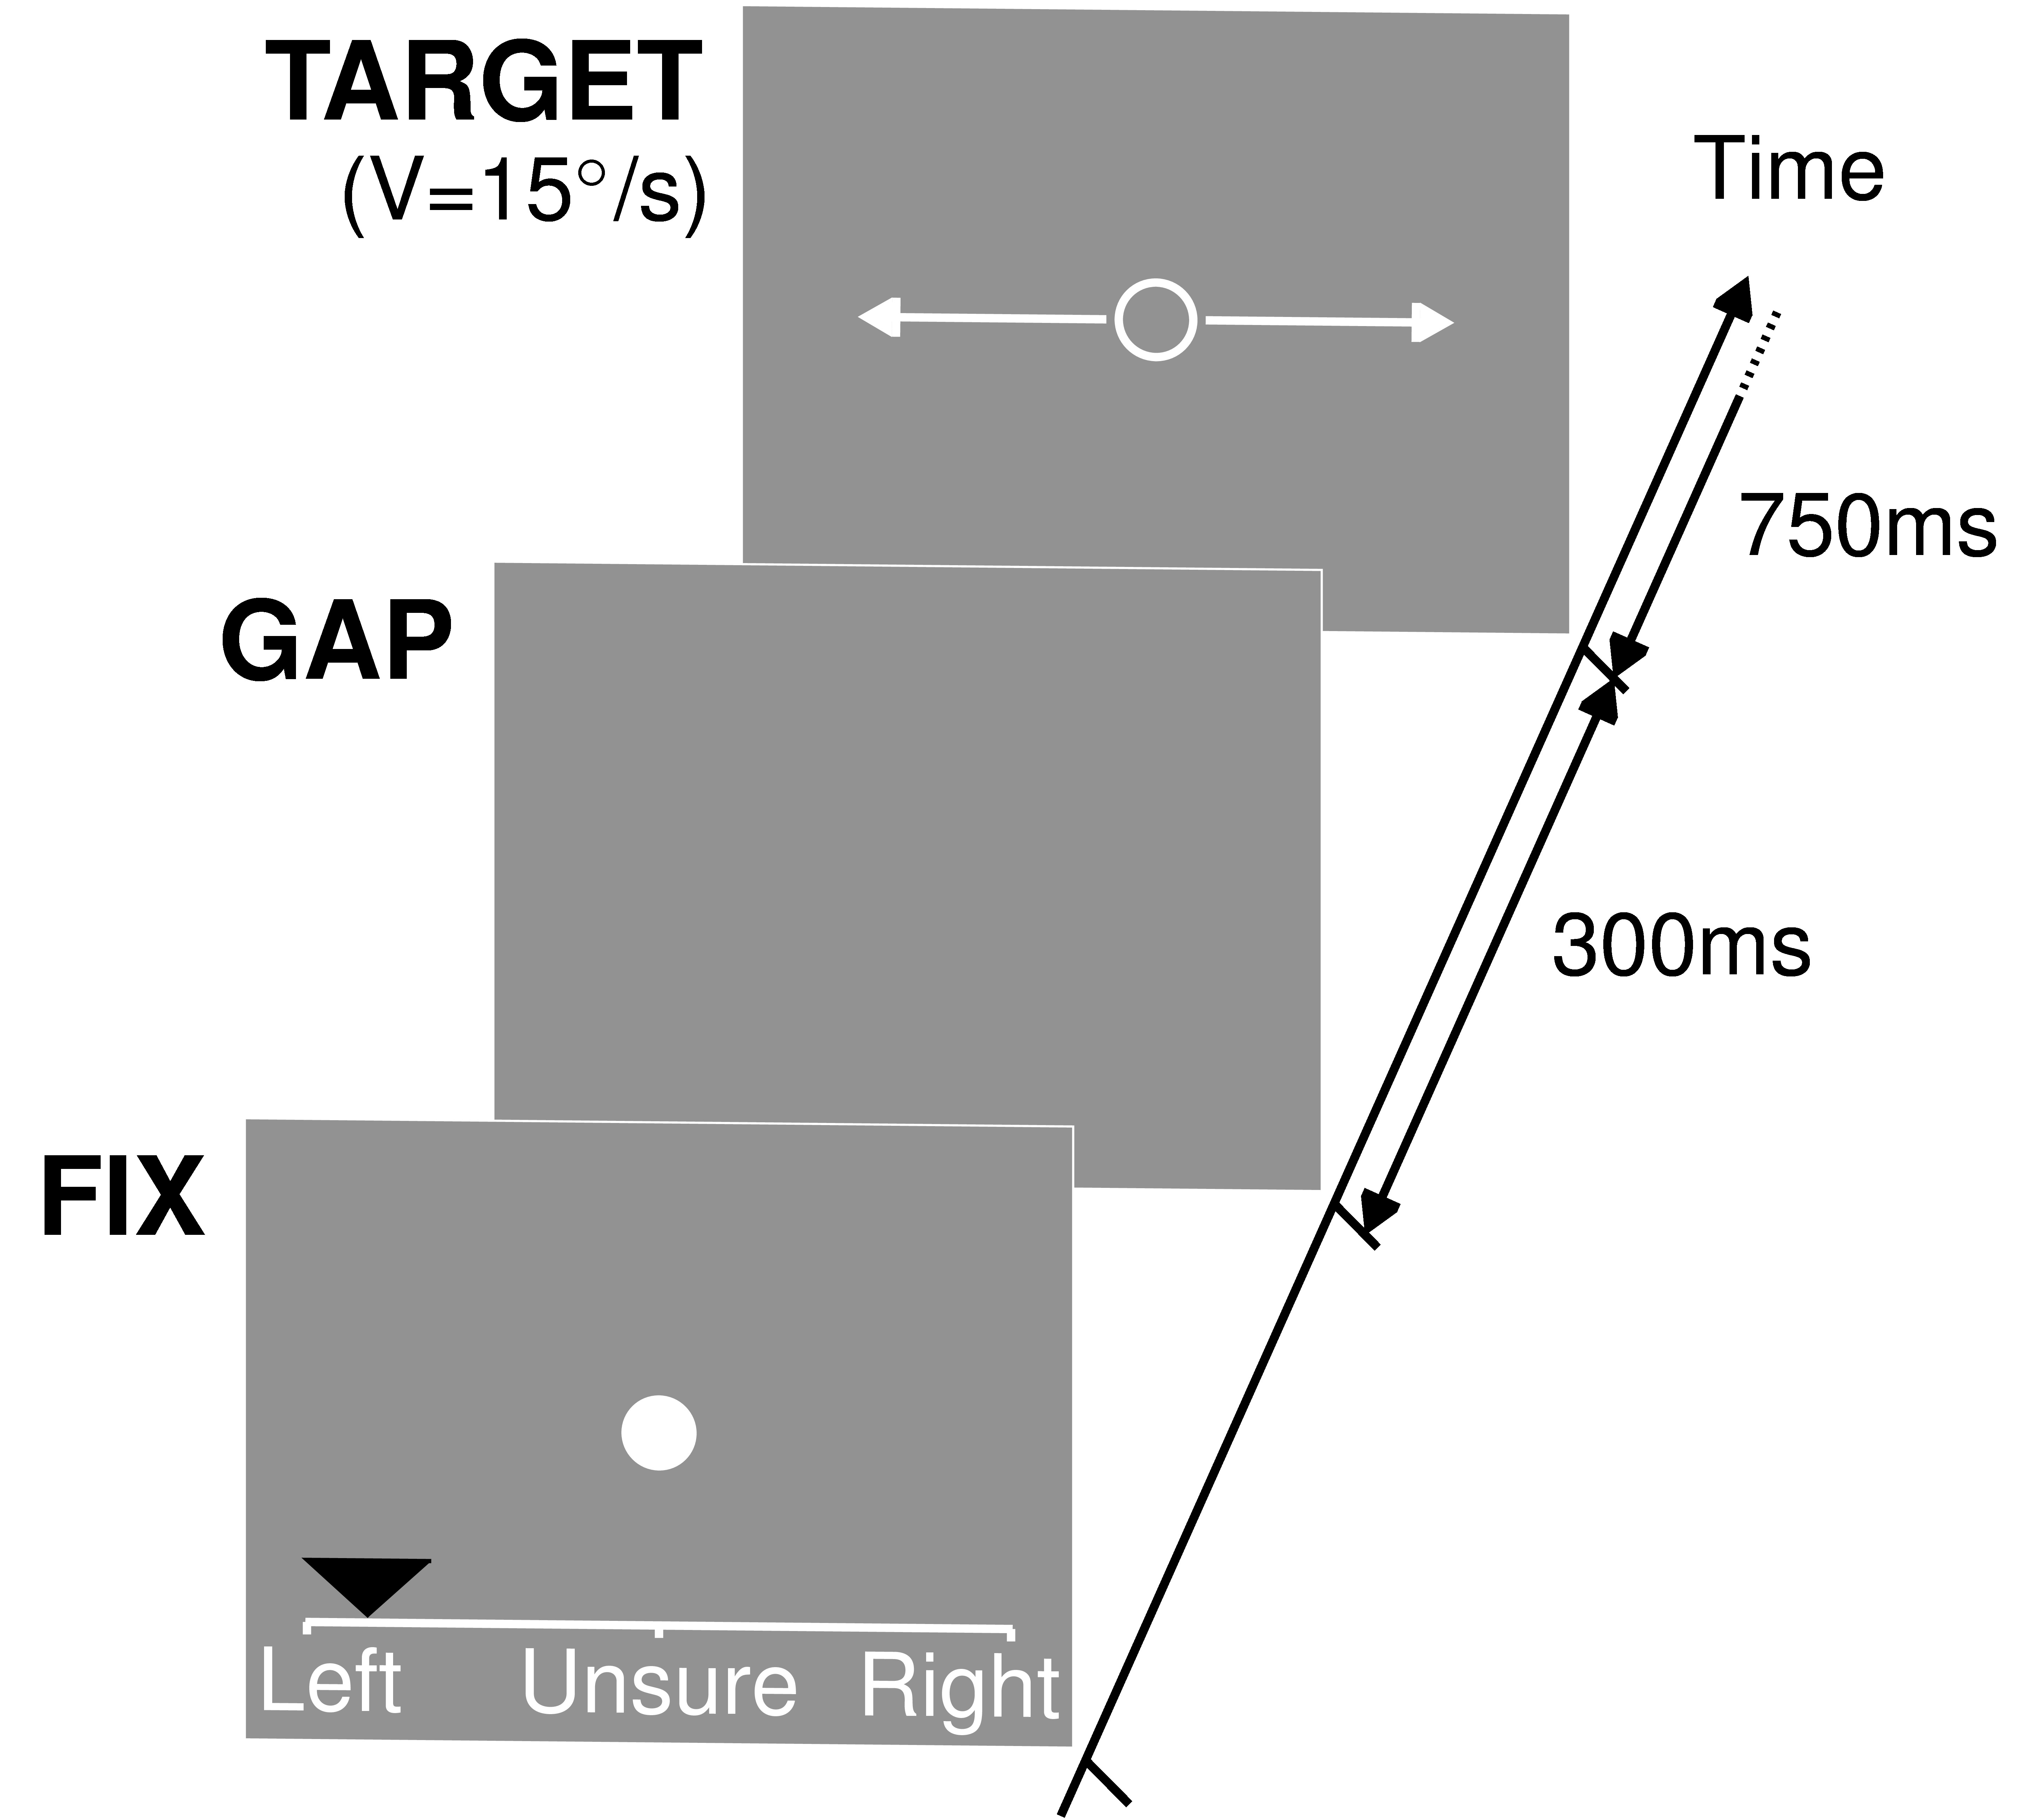
\includegraphics[width=0.350\linewidth]{1_C_protocol_bet}};
\draw [anchor=north west] (0.000\linewidth, .62\linewidth) node {$\mathsf{(A)}$};
\draw [anchor=north west] (0.350\linewidth, .62\linewidth) node {$\mathsf{(B)}$};
\draw [anchor=north west] (0.665\linewidth, .62\linewidth) node {$\mathsf{(C)}$};
\end{tikzpicture}
}
\caption{
\textbf{Smooth pursuit eye movements and explicit direction predictions in a volatile switching environment}
We test the capacity of human participants to adapt to a volatile environment.
\textit{(A)}~
We use a 3-layered generative model of fluctuations in target directions (TD)
that we call the Binary Switching model.
This TD binary variable is chosen using a Bernoulli trial of a given probability bias.
This probability bias is constant for as many trials until a switch is generated.
At a switch, the bias is chosen at random from a given prior.
Switches are generated in the third layer as binary events drawn from a Bernoulli trial
with a given hazard rate (defined here as $1/40$ per trial). We show one realization of a block of $200$ trials.
\textit{(B)}~
The eye-movements task was an adapted version of a task developed by~\citet{Montagnini2010}.
Each trial consisted of sequentially:
a fixation dot (FIX, of random duration between $400$ and $800$~\ms),
a blank screen (GAP, of fixed duration of  $300$~\ms) and
a moving ring-shaped target (TARGET, with $15~\degree/s$ velocity) which the observers were instructed to follow.
The direction of the target (right or left) was drawn pseudo-randomly
according to the generative model defined above.
\textit{(C)}~In order to titrate the adaptation
to the environmental volatility of target direction at the explicit and conscious level,
we invited each observer to perform on a different day a new variant of the direction-biased experiment,
where we asked participants to predict, \emph{before each trial}, %the level of confidence for
their estimate of the forthcoming direction of the target.
As shown in this sample screenshot,
this was performed by moving a mouse cursor (black triangle) on a continuous rating scale
between ``Left'', to ``Unsure'' and finally ``Right''.
}
\label{fig:intro}
\end{figure}
%-------------------------------------------------------------%
%: limits of the previous method
%In order to generalize such results to more ecological conditions,
%it is thus necessary to extend the experimental protocol of~\citet{Montagnini2010} in three aspects that will be illustrated in the next section.
% ------------------------------------------------------------------
\subsection{Contributions}%Outline}
% ------------------------------------------------------------------
%: 1C : what is novel in our work
% ------------------------------------------------------------------
%: 1Ca how we do it : or rather why we do it this way (and not like Matthys)
The goal of this study is to generalize the adaptive process
observed in anticipatory pursuit~\citep{Montagnini2010,SantosKowler2017}
to more ecological settings and
also to broaden its scope by showing that such adaptive processes
occur also at an explicit level.
We already mentioned that by manipulating the probability bias for target motion direction,
it is possible to modulate the strength (direction and mean velocity) of anticipatory pursuit.
This suggests that probabilistic information about direction bias may be used
to inform the internal representation of motion prediction
for the initiation of anticipatory movements.
However, %it is yet unclear what generative model to use
previous studies have overlooked the importance to design a realistic generative model to dynamically manipulate the probability bias
and generate an ecologically relevant input sequence of target directions.
A possible confound comes from the fact that
previous studies have used fixed-lengths sequences of trials, % (\textit{trial blocks}),
stacked in a sequence of conditions defined by the different probability biases.
Indeed, observers may potentially pick up
the information on the block's length
to predict the occurrence of a switch (a change in probability bias) during the experiment.
Second, we observed qualitatively that following a switch,
the amplitude of anticipatory pursuit velocity changed gradually,
consistently with other adaptation paradigms~\citep{Fukushima1996,Kahlon1996,Souto13}.
The estimate of the characteristic temporal parameters for this adaptation mechanism
may become particularly challenging in a dynamic context,
where the probabilistic contingencies vary in time in an unpredictable way.
Finally, whether and how the information processing underlying
the buildup of anticipatory pursuit and its dynamics is linked to
an explicit estimate of probabilities is still largely unknown.

%%%-------------------------------------------------------------%
%: 1Cb design of the binary switching generative model
To assess the dynamics of the adaptive processes
which compensate for the variability within sensory sequences,
one may generate random sequences of Target Directions (TDs)
using a dynamic value for the probability bias $p = \text{Pr}(\text{TD is 'right'})$,
with a parametric mechanism controlling for the volatility at each trial.
In the Hierarchical Gaussian Filter model~\citep{Mathys11}, for instance,
volatility is controlled as a non-linear transformation
of a random walk (modeled itself by a Brownian motion with a given diffusion coefficient).
% \Rone{line 192: Is it meant to be "volatility" and not "variability"?}
Ultimately, this hierarchical model allows to generate a sequence of binary choices
where volatility is controlled by %fluctuating the variability along a given trajectory.
a specific random variable which fluctuates in time according to some probabilistic law.
Such a forward probabilistic model is invertible
using some simplifying assumptions and allows
to extract a time-varying inference of the agent's belief about volatility~\citep{Vossel14}.
% \Rone{line 195-197 the term trial block may lead to some confusion, as it is meant to be the sequence of trials with the same probability but also commonly the number of trials in a full sequence.}
Herein, to explicitly analyze the effect of history length,
we rather extend the protocol of~\citet{Montagnini2010} such that the probability bias
is still fixed within sub-blocks but that these sub-blocks have variable lengths,
that is, by introducing switches occurring at random times.
Therefore, similarly to~\citet{Meyniel13}, we use a model for which
the bias $p$ in target direction varies according to a piecewise-constant function.
We expect that within each of these sub-blocks that we defined,
the uncertainty about of the value of $p$
will progressively decrease as we accumulate trials.
In addition, the range of possible biases was finite ($p \in \{0, .1, .25, .5, .75, .9, 1\}$) in our previous study.
In the present work, we also extend the paradigm
by drawing $p$ as a continuous random variable
within the whole range of possible probability biases (that is, the segment $[ 0, 1 ]$).

%: 1Cc  equations
As a summary, we first draw random events (that we denote as ``switches'')
with a given mean frequency (the ``hazard rate'') and which controls the strength of the volatility.
Second, the value $p$ of the bias only changes at the moment of a switch,
independently of the previous bias' value
and it is stationary between two switches, forming what we call an ``epoch''.
Third, target direction is drawn as a Bernoulli trial using the current value of $p$.
Such a hierarchical structure is presented in~\seeFig{intro}-A,
where we show the realization of the target's directions sequence,
the trajectory of the underlying probability bias (hidden to the observer), and
the occurrences of switches.
Mathematically, this can be considered as a three-layered hierarchical model
defining the evolution of the model at each trial $t$ as the vector  $(x_2^t, x_1^t, x_0^t)$.
At the topmost layer,
the occurrence $x_2^t \in \{ 0, 1 \}$ of a switch ($1$ for true, $0$ for false)
is  drawn from a Bernoulli trial $\Bb$ parameterized by its hazard rate $h$
(as the frequency of occurrence for each trial).
The value of $\tau=\frac 1 h$ thus gives the average duration (in number of trials)
between the occurrence of two switches.
In the middle layer, the probability bias $p$ of target direction
is a random variable that we define as $x_1^t \in [0, 1]$.
It is chosen at random from a prior distribution $\Pp$
%(that will be described in more detail in the following sections)
at the moment of a switch,
and else it is constant until the next occurrence of a switch.
The prior distribution $\Pp$ can be for instance
the uniform distribution $\Uu$ on $ [ 0, 1 ] $ or
Jeffrey's prior $\Jj$~(see \seeApp{bcp}).
Finally, a target moves either to the left or to the right,
and we denote this variable (target direction, TD) as $x_0^t \in \{ 0, 1 \}$.
This direction is drawn from a Bernoulli trial
parameterized by the direction bias $p=x_1^t$.
In short, this is described according to the following equations:
%\begin{itemize}
%    \item Occurrence of a switch: $x_2^t \propto \Bb(h)$
%    \item Dynamics of probability bias: \eql{\choice{\text{if} \quad x_2^t=0 \quad \text{then} \quad  x_1^t = x_1^{t-1} \\
%\text{else} \quad x_1^t \propto \Pp  }\label{eq:bsm}}
%    \item Sequence of directions:  $x_0^t \propto \Bb(x_1^t)$
%\end{itemize}
 \eql{\choice{
\text{Occurrence of a switch: } x_2^t \propto \Bb(1/\tau) \\
 % TODO: nest the choice
\text{Dynamics of probability bias $p=x_1^t$ }
 \choice{\text{if} \quad x_2^t=0 \quad \text{then} \quad  x_1^t = x_1^{t-1} \\
 \text{else} \quad x_1^t \propto \Pp  \\
 } \\
\text{Sequence of directions: } x_0^t \propto \Bb(x_1^t)
 }\label{eq:bsm}}
In this study, we generated a sequence of $600$ trials,
and there is by construction a switch at $t=0$ (that is, $x_2^0=1$).
In addition, we imposed in our sequence that a switch
occurs after trial numbers $200$ and $400$,
in order to be able to compare adaptation properties
across these three different trial blocks.
%The model generating the experimental sequence of trial directions, as well as the experimental protocol are illustrated in~\seeFig{intro}-A.
With such a three-layered structure, the model generates the randomized occurrence of switches,
itself generating epochs with constant direction probability %between two switches separated by a random length
%and chosen in the continuous range of possible biases' values,
and finally the random sequence of Target Direction (TD) occurrences at each trial.
This system of three equations defined in~\seeEq{bsm}
defines the Binary Switching model
which we used for the generation of experimental sequences presented to human participants in the experiments.
We will use that generative model as the basis for an ideal observer model equipped to
invert that generative model in order to estimate the time-varying probability bias for a given sequence of observations (TDs).
The comparison of human behavior with the ideal observer model's predictions will allow us to test it as a model for the adaptation of human behavior to the environment's volatility.

%: 1Cd outline
This paper is organized in five parts.
After this introduction where we presented the motivation for this study,
the next section~(\seeSec{Bayesian_change_point}) will present
an inversion of the (forward) binary switching generative model,
coined the Binary Bayesian Change-Point (BBCP) model.
To our knowledge, such algorithm was not yet available, and
we will here provide with an exact analytical solution
by extending previous results from~\citet{AdamsMackay2007}
to the binary nature of data in the Binary Switching model presented above (see~\seeEq{bsm}).
In addition, the proposed algorithm is biologically realistic
as it uses simple computations and is \emph{online},
that is, all computations on the sequence may be done
using solely a set of variables available at the present trial,
compactly representing all the sequence history seen in previous trials.
We will also provide a computational implementation
and a quantitative evaluation of this algorithm.
Then, we will present in~\seeSec{results_psycho} the analysis of experimental evidence
to validate the generalization of previous results %.
with this novel switching protocol.
In order to understand the nature of
the representation of motion regularities underlying adaptive behavior,
we collected both
the recording of eye movements
and the verbal explicit judgments about expectations on motion direction.
In one session, participants were asked to estimate
``how much they are confident that
the target will move to the right or left in the next trial'' and
to adjust the cursor's position on the screen accordingly~(see \seeFig{intro}-C).
In the other experimental session on a different day,
we showed the same sequence of target directions and
recorded participants' eye movements~(see \seeFig{intro}-B).
Combining these theoretical and experimental results,
a novelty of our approach is to use the BBCP agent as a regressor
which will allow us to match experimental results
and to compare its predictive power compared to classical models such as the leaky integrator model.
Hence, we will show that behavioral results match best with the BBCP model.
In~\seeSec{inter}, we will synthesize these results
by inferring the volatility parameters inherent to the models
by best-fitting it to each each individual participant.
This will allow the analysis of inter-individual behavioral responses for each session.
In particular, we will test if one could extract observers' prior (preferred) volatility,
that is, a measure of the dynamic compromise between
exploitation (``should I stay?'') and exploration (``should I go?'')
for the two different sessions challenging predictive adaptive processes
both at the implicit and explicit levels.
Finally, we will summarize and conclude this study and
offer some perspectives for future work in~\seeSec{outro}.
%
%: %%%%%%%%%%%%%%%%%%%%%%%%%%%%%%%%%%%%%%%%%%%%%%%%%%%%%%%%%%%%%%%
\section{Results: Binary Bayesian Change-Point (BBCP) detection model}
%%%%%%%%%%%%%%%%%%%%%%%%%%%%%%%%%%%%%%%%%%%%%%%%%%%%%%%%%%%%%%%%
%%%%%%%%%%%%%%%%%%%%%%%%%%%%%%%%%%%%%%%%%%%%%%%%%%%%%%%%%%%%%%%%
\label{sec:Bayesian_change_point}
%%%%%%%%%%%%%%%%%%%%%%%%%%%%%%%%%%%%%%%%%%%%%%%%%%%%%%%%%%%%%%%%
%
%: 2 short intro
%
As we saw above, Bayesian methods provide a powerful framework for studying human behavior and adaptive  processes in particular.
For instance,~\citet{Mathys11} first defined a multi-layered generative model for
sequences of input stimuli.
By inverting this stochastic forward process,
they could extract relevant descriptors at the different levels of the model
and fit these parameters with the recorded behavior.
Here, we use a similar approach, focusing specifically on the binary switching generative model,
as defined in~\seeEq{bsm}.
To begin, we define as a control a first ideal observer, the \textit{leaky integrator} (or \textit{forgetful agent}),
which has an exponentially-decaying memory for the events that occurred in the past trials.
This agent can equivalently be described as one
which assumes that volatility is stationary with a fixed characteristic frequency of switches.
Then, we extend this model to an agent
which assumes the existence of (randomly occurring) switches, that is,
that the agent is equipped with the prior knowledge
that the value of the probability bias may change
at specific (yet randomly drawn) trials,
as defined by the forward probabilistic model in~\seeEq{bsm}.
%
% ------------------------------------------------------------------
\subsection{Forgetful agent (Leaky integrator) detection model}%
% ------------------------------------------------------------------
%: 2Aa justification from previous studies
The leaky integrator ideal observer represents a classical, widespread and
realistic model of how trial-history shapes
adaptive processes in human behavior~\citet{Anderson2006}.
It is also well adapted to model motion expectation in the direction-biased experiment which leads to anticipatory pursuit.
In this model, given the sequence of observations $x_0^t$ from trial $0$ to $t$,
the expectation $p=\hat{x}_1^{t+1}$ of the probability for the next trial direction can be modeled by making a simple heuristic~\citep{Anderson2006}:
This probability is the weighted average of
the previously predicted probability, $\hat{x}_1^{t}$, with the new information $x_0^t$,
where the weight corresponds to a leak term (or discount)
equal to $(1 - h)$, with $h \in [0, 1]$.
At trial $t$, this model can be expressed with the following equation:
\eql{
\hat{x}_1^{t+1} = (1 - h) \cdot \hat{x}_1^{t} + h \cdot x_0^t
\label{eq:leaky}}
where $\hat{x}_1^{t=0}$ is equal to some prior value ($0.5$ in the unbiased case),
corresponding to the best guess at $t=0$ (prior to the observation of any data).
% NOTE: it's an AR(1) process https://stats.stackexchange.com/questions/358162/writing-ar1-as-a-ma-infty-process

%: from heuristics to ideal observer
In other words, the predicted probability $\hat{x}_1^{t+1}$ is computed
from the integration of previous instances
with a progressive discount of past information.
The value of the scalar $h$ represents
a compromise between responding rapidly
to changes in the environment ($h \approx 1$) and
not prematurely discarding information still of value
for slowly changing contexts  ($h \approx 0$).
For that reason, we call this scalar the hazard rate
in the same way to that defined for the binary switching generative model presented above (see~\seeEq{bsm}).
Moreover, one can define $\tau = 1 / h$ as
a characteristic time (in units of number of trials)
for the temporal integration of information.
Looking more closely at this expression,
the ``forgetful agent'' computed in \seeEq{leaky}
consists of an exponentially-weighted moving average (see \seeApp{leaky}).
It may thus be equivalently written in the form of a time-weighted average:
\eql{
\hat{x}_1^{t+1} = (1-h)^{t+1} \cdot \hat{x}_1^{t=0} + h \cdot \sum_{0\leq i \leq t} (1 - h)^{i} \cdot x_0^{t-i}
\label{eq:leaky2}}
The first term corresponds to the discounted effect of the prior value,
which tends to $0$ as $t$ increases.
More importantly, as $1-h < 1$, the second term corresponds to the \emph{leaky} integration of novel observations.
Inversely, let us now assume that
the true probability bias for direction changes randomly with a mean rate of once
every $\tau$ trials: $Pr(x_2^t=1)=h$.
As a consequence, the probability that the bias does not change is $Pr(x_2^t=0)=1-h$ at each trial.
Assuming independence of these occurrences, the predicted probability $p=\hat{x}_1^{t+1}$ is thus proportional to the sum
of the past observations weighted by the belief that the bias has not changed during $i$ trials in the past, that is, exactly as defined by the second term of the right-hand side in~\seeEq{leaky2}.
This shows that assuming that changes occur at a constant rate ($\hat{x}_2^t=h$)
but ignoring more precise information on the temporal occurrence of the switch,
the optimal solution to this inference problem is the
ideal observer defined in~\seeEq{leaky2},
which finds an online recursive solution in~\seeEq{leaky}.
We therefore proved here that the heuristic derived for the leaky integrator
is an exact inversion of the two-layered generative model
which assumes a constant epoch-duration between switches of the probability bias.

%: 2Ac  using \hat{p} as a regressor & limits of the leaky integrator
The correspondence that we proved between the weighted moving average heuristic
and the forgetful agent model as an ideal solution to that generative model leads
us to several interim conclusions.
First, the time series of inferred $\hat{x}_1^{t+1}$ values
can serve as a regressor for behavioral data
to test whether human observers follow a similar strategy.
% \Rone{I can't make much sense of 324-326. The point that Equation 3 assumes a constant weight is also obscure to me. Doesn't a leaky-integrator amount to weighting past trials depending on trial number? This needs to be clarified.}
In particular, the free parameter of the model ($h$),
may be fitted to the behavioral dataset.
Testing different hypothesis for the value of $h$ thus allows
to infer the agents' most likely belief in the (fixed) weight decay.
%for instance to the data shown in~\seeFig{results_intro}.
Now, since we have defined a first generative model
and the corresponding ideal observer (the forgetful agent),
we next define a more complex model,
in order to overcome some of the limits of the leaky integrator.
Indeed, a first criticism could be that
this model is too rigid and does not sufficiently
account for the dynamics of contextual changes~\citep{Behrens07}
as the weight decay corresponds to assuming \emph{a priori} a constant precision in the data sequence, contrary to more elaborate Bayesian models~\citep{Vilares2011}.
It seems plausible that the memory size (or history length) used by the brain
to infer any event probability can vary, and that this variation could be related
to an estimate of environmental volatility as inferred from past data.
The model presented in~\seeEq{leaky2} uses a constant weight
% (decaying with the temporal distance from the current trial)
for all trials, while the actual precision of each trial
can be potentially evaluated and used
for precision-weighted estimation of the probability bias.
To address this hypothesis, our next model is inspired
by the Bayesian Change-Point detection model~\citep{AdamsMackay2007}
of an ideal agent
inferring the trajectory in time of the probability bias ($x_1^t$),
but also predicting the probability $Pr(x_2^t=1)$ of the occurrence of switches.
% ------------------------------------------------------------------
\subsection{Binary Bayesian Change-Point (BBCP) detection model}
% ------------------------------------------------------------------
\label{sec:Binary_Bayesian_change_point}
%-------------------------------------------------------------%
%: FIGURE 3 fig:Bayesianchangepoint \seeFig{Bayesianchangepoint}
\begin{figure}%[b!]
% cf 3_Results_2.ipynb
\centering{
\begin{tikzpicture}[thick,scale=.95]
\node [anchor=north west]  (imgA) at (0.\linewidth,.55\linewidth){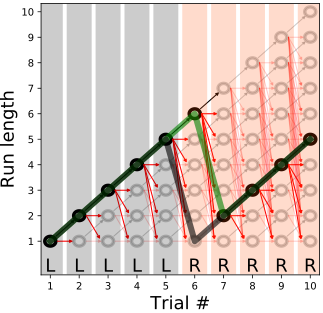
\includegraphics[width=0.33
\linewidth]{3_BCP_model}};
\node [anchor=north west]  (imgB) at (0.36\linewidth,.580\linewidth){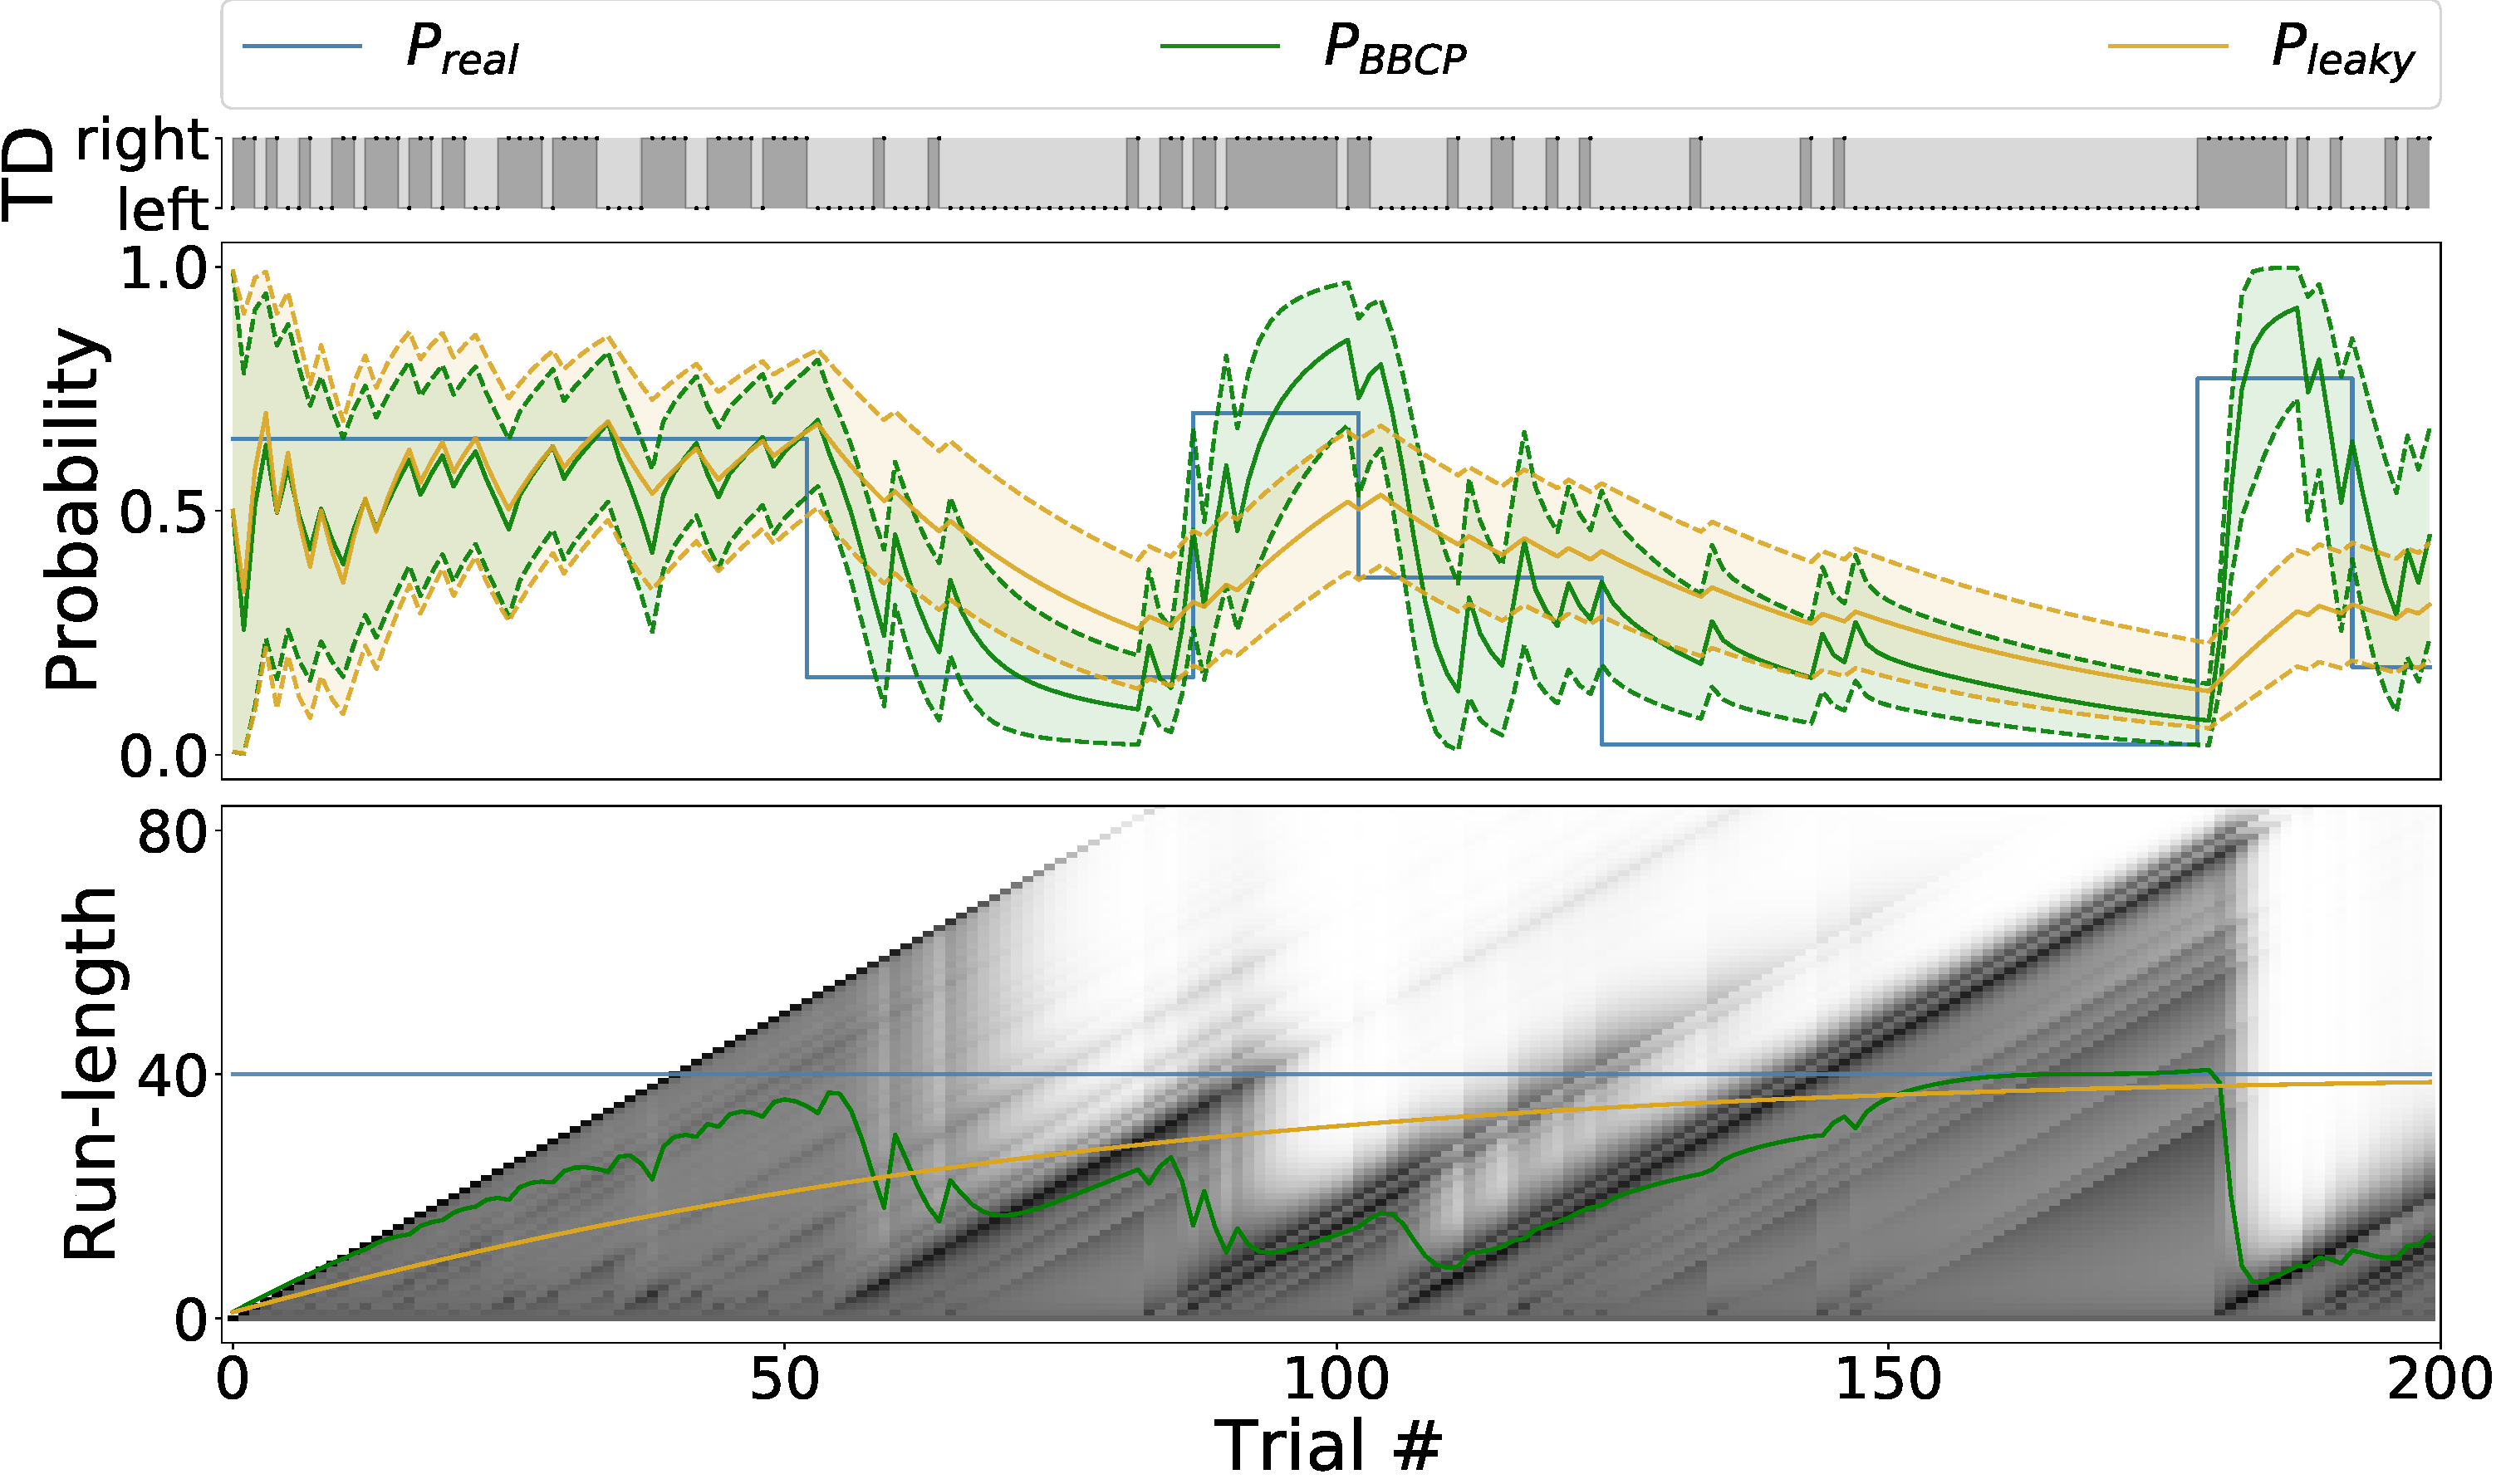
\includegraphics[width=0.64\linewidth]{3_BCP_readouts}};
\draw [anchor=north west] (0.000\linewidth, .62\linewidth) node {$\mathsf{(A)}$};
\draw [anchor=north west] (0.382\linewidth, .62\linewidth) node {$\mathsf{(B)}$};
\end{tikzpicture}
}
\caption{\textbf{Binary Bayesian Change-Point (BBCP) detection model.}
~\textit{(A)}
This plot shows a synthesized sequence of $13$ events,
either a leftward or rightward movement of the target (TD).
Run-length estimates are expressed as hypotheses about the length of an epoch
over which the probability bias was constant,
that is, the number of trials since the last switch.
Here, the true probability bias switched from a value of $.5$ to $.9$ at trial $7$,
as can be seen by the trajectory of the true run-length (blue line).
The BBCP model tries to capture the occurrences of a switch
by inferring the probability of different possible run-lengths.
At any new datum (trial), this defines a Hidden Markov Model
as a graph (trellis), where % of possible run-lengths.
edges indicate that a message is being passed
to update each node's probability (as represented by arrows from trial $13$ to $14$).
Black arrows denote a progression of the run-length at the next step (no switch),
while gray lines stand for the possibility that a switch happened:
In this case the run-length would fall back to zero.
The probability for each node is represented by the grey scale (darker grey colors denote higher probability)
and the distribution is shown in the inset for two representative trials: $5$ and $11$.
Overall, this graph shows how the model integrates information to accurately identify a switch
and produce a prediction for the next trial (e.g. for $t=14$).
%The black \CP{Bleu} [and green] \CP{plus de courbe verte} curve respectively represent
%the actual [and inferred] run-length of the simulated data
%as a function of trial number.
%In this instance, the inferred switch is delayed
%by one trial with respect to the true switch.
%\CP{representation des valeurs du run-length en haut a gauche pour les essais 5 (en gris) et 8 (en bleu), on peut voir que pour l'essais 5 et 8 la probabilit\'e qu'il n'y est pas eu de switch depuis le d\'ebut est la plus importante (peut \^etre prendre un autre essais plus parlant - trial 10: proba switch à l'essais 5 est plus importante (notebook3) ?)}
~\textit{(B)} On a longer sequence of $200$ trials,
representative of a trial block of our experimental sequence (see~\seeFig{intro}-A), % and~\seeFig{results_raw}),
we show %in the top plot
the actual events which are observed by the agent (TD),
along with the (hidden) dynamics of the true probability bias $P_{\text{true}}$ (blue line),
the value inferred by a leaky integrator ($P_{\text{leaky}}$, orange line)
and the results of the BBCP model
in estimating the probability bias $P_{\text{BBCP}}$ (green line),
along with $.05$ and $.95$ quantiles (shaded area).
This shows that for the BBCP model,
the accuracy of the predicted value of the probability bias
is higher than for the leaky integrator.
Below, we show the belief (as grayscales) for the different possible run-lengths.
%as a function of the trial number.
%A darker color denotes a higher probability.
The green and orange line correspond to the mean run-length which is inferred,
respectively, by the BBCP and leaky models:
Note that in the BBCP, while it takes some trials to detect switches,
they are in general correctly identified (transitions between diagonal lines) and
that integration is thus faster than for the leaky integrator,
as illustrated by the inferred value of the probability bias.
}
\label{fig:Bayesianchangepoint}
\end{figure}
%-------------------------------------------------------------%
%-------------------------------------------------------------%
%: 2Ba precision in our belief of \hat{p}
%-------------------------------------------------------------%
There is a crucial difference between the forgetful agent presented above
%\AM{WE CAN SKIP THIS:which believes that changes occur at a constant rate ($\hat{x}_2^t=h$, see~\seeEq{leaky2})}
and an ideal agent which would invert the (generative) Binary Switching model (see~\seeEq{bsm}).
Indeed, at any trial during the experiment,
the agent may infer beliefs about the probability of the volatility $x_2^t$
which itself is driving the trajectory of the probability bias $x_1^t$.
Knowing that the latter is piece-wise constant,
an agent may have a belief over the number of trials since the last switch.
This number, that is called the \emph{run-length} $r^t$~\citep{AdamsMackay2007}, is useful in two manners.
First, it allows the agent to restrict the prediction $\hat{x}_1^{t+1}$ of $x_1^{t+1}$
only based on those samples produced since the last switch, from $t-r^t$ until $t$.
% and which we denote as $x_0^{(r^t)}=x_0^{r^t:t}$ .
Indeed, the samples $x_0^t$ which occurred before the last switch
were drawn independently from the present true value $x_1^t$
and thus cannot help estimating the latter.
As a consequence, the run-length is a latent variable
that captures at any given trial all the hypotheses that may be occurring.
Second, it is known that for this estimate, the precision
(that is, the inverse of variance) on the estimate $\hat{x}_1^{t+1}$
grows linearly with the number of samples:
The longer the run-length, the sharper the corresponding (probabilistic) belief.
We have designed an agent inverting the binary switching generative model by extending
the Bayesian Change-Point (BCP) detection model~\citep{AdamsMackay2007}.
The latter model defines the agent as an inversion of a switching generative model
for which the observed data (input) is Gaussian.
We present here an exact solution for the case of the Binary Switching model,
that is, for which the input is binary (here, left or right). %

%-------------------------------------------------------------%
%: 2Bb prediction / update cycle
%-------------------------------------------------------------%
In order to define in all generality the change-point (switch) detection model,
we will initially describe the fundamental steps leading to its construction,
while providing the full algorithmic details in~\seeApp{bcp}.
%  by~\seeEq{run_length} (more details on this derivation in~\seeApp{bcp})
The goal of predictive processing at trial $t$
is to infer the probability $Pr(x_0^{t+1} | x_0^{0:t})$ of the next datum
knowing what has been observed until that trial
(that we denote by $x_0^{0:t} = \{ x_0^0, \ldots, x_0^t \}$).
This prediction uses the agent's prior knowledge
that data is the output of a given (stochastic) generative model (here, the Binary Switching model).
To derive a Bayesian predictive model, we introduce
the run-length as a latent variable which gives to the agent the possibility to represent
different hypotheses about the input.
We therefore draw a computational graph (see \seeFig{Bayesianchangepoint}-A) where, at any trial,
an hypothesis is formed on as many ``nodes'' than there are run-lengths.
Note that run-lengths may be limited by the total number of trials $t$.
%
%This is for instance the task that we defined
%for the bet experiment, where each participant
%was asked to report their level of confidence for the next outcome
%for the next trial.
%
%Using the run-length $r^t$ as a latent variable at each trial $t$,
%we define the distribution which represents our belief
%for all different hypotheses on $r^t$.
%which
As a readout, we can use this knowledge of the predictive probability conditioned on the run-length,
such that one can compute the marginal predictive distribution:
\eql{
Pr(x_0^{t+1} | x_0^{0:t}) =
%\sum_{r^{t}} \beta^{(r)}_t \cdot Pr(x_0^t | r^{t}, x_0^{0:t-1})
%\sum_{r^{t}} Pr(x_0^{t+1} | r^{t}, x_0^{0:t}) \cdot Pr(r^t | x_0^{0:t})
%\sum_{r^{t}} Pr(x_0^{t+1} | x_0^{(r^{t})}) \cdot \beta^{(r)}_t
\sum_{r^{t}\geq 0} Pr(x_0^{t+1} | r^{t}, x_0^{0:t}) \cdot \beta^{(r)}_t
\label{eq:pred}
}
where $Pr(x_0^{t+1} | r^{t}, x_0^{0:t})$ is the probability of
the Bernoulli trial modeling the outcome of a future datum $x_0^{t+1}$,
conditioned on the run-length and
$\beta^{(r)}_t=Pr(r^t | x_0^{0:t})$ is the probability for each possible run-length given the observed data.
Note that we know that, at any trial, there is a single true value for this variable $r^{t}$
and that $\beta^{(r)}_t$ thus represents the agent's inferred probability distribution over the run-length $r$.
As a consequence, $\beta^{(r)}_t$ is scaled such that $\sum_{r \geq 0 } \beta^{(r)}_t = 1$.
%a previous value $Pr(x_0^{t} | r^{t-1}, x_0^{0:t-1})$
%and the likelihood associated to the new value $x_0^t$.
%-------------------------------------------------------------%
%: 2Bc prediction cycle
%-------------------------------------------------------------%
%-------------------------------------------------------------%
% Computing sufficient statistics
%-------------------------------------------------------------%

With these premises, we define the BBCP
as a prediction / update cycle
which connects nodes from the previous trial to that at the current trial.
Indeed, we will \emph{predict} the probability
$\beta^{(r)}_t$ at each node, knowing either an initial prior, or its value on a previous trial.
In particular, at the occurrence of the first trial, we know for certain that there is a switch and
initial beliefs are thus set to the values $\beta^{(0)}_0=Pr(r^t=0)=1$ and
$\forall r>0$, $\beta^{(r)}_0=Pr(r^0=r)=0$.
Then, at any trial $t>0$, as we observe a new datum $x_0^t$,
we use a knowledge of $\beta^{(r)}_{t-1}$ at trial $t-1$,
the likelihood $\pi^{(r)}_{t}=Pr(x_0^{t} | r^{t-1}, x_0^{0:t-1})$  and
the transition probabilities defined by the generative model
to predict the beliefs over all nodes: %

\eqa{
\beta^{(r)}_t \propto \sum_{r^{t-1} \geq 0} \beta^{(r)}_{t-1} \cdot Pr(r^t | r^{t-1}) \cdot  \pi^{(r)}_{t}
\label{eq:pred_node}
}
In the computational graph, % (\seeFig{Bayesianchangepoint}-A),
\seeEq{pred_node} corresponds to a message passing from the nodes at time $t-1$
to that at time $t$. % and formalized by the transition matrix $Pr(r^t | r^{t-1})$.
We will now detail how to compute the transition probabilities and the likelihood.

%In the second step, one can perform prediction
%using the graph defined in \seeFig{Bayesianchangepoint}-A.
%Now that we have the vector of likelihoods $\pi^{(r)}_t=\Ll(x_0^t |  \mu^{(r)}_{t}, \nu^{(r)}_{t})$,
%one can update probabilities and perform the next prediction for trial $t+1$.
First, knowing that the data is generated by the Binary Switching model (see~\seeEq{bsm}),
the run-length is either null at the moment of a switch,
or its length (in number of trials) is incremented by $1$ if no switch occurred:

\eql{\choice{
\text{if} \quad x_2^t=1 \text{,} \quad r^t = 0\\
\text{else} \quad x_2^t=0 \text{,} \quad r^t = r^{t-1} +1 }\label{eq:run_length}}%see~\seeEq{run_length}
%\text{and else} \quad r^t = r^{t-1} +1 }\label{eq:run_length}}%see~\seeEq{run_length}
This may be illustrated by a graph
in which information will be represented at the different nodes for each trial $t$.
%In a switching model like the BSM, the transition matrix % defined by the graph,
This defines the transition matrix $Pr(r^t | r^{t-1})$
as a partition in two exclusive possibilities:
Either there was a switch or not.
It allows us to compute the \emph{growth probability} for each run-length. % $r \geq 0$.
On the one hand, the belief of an increment of the run-length at the next trial is: %, before observing a new datum:

\eqa{
\beta^{(r+1)}_t = \frac{1}{B} \cdot \beta^{(r)}_{t-1} \cdot \pi^{(r)}_{t} \cdot (1-h)
\label{eq:beta_noswitch}
}
where $h$ is the scalar defining the hazard rate.
On the other hand, it also allows to express the change-point probability as:

\eqa{
\beta^{(0)}_t  = \frac{1}{B} \cdot \sum_{r \geq 0} \beta^{(r)}_{t-1} \cdot \pi^{(r)}_{t} \cdot h
\label{eq:beta_switch}
}
with $B$ such that $\sum_{r \geq 0} \beta^{(r)}_{t} = 1$.
Note that $\beta^{(0)}_t=h$ and thus $B=\sum_{r \geq 0} \beta^{(r)}_{t-1} \cdot \pi^{(r)}_{t}$.
%This finalizes the prediction step.
Knowing this probability strength and the previous value of the prediction, % an estimate for our belief on the different variables at the previous trial $t-1$,
we can therefore make a prediction for our belief of the probability bias at the next trial $t+1$,
prior to the observation of a new datum $x_0^{t+1}$ and resume the prediction / update cycle (see Equations~\ref{eq:pred},~\ref{eq:beta_noswitch} and~\ref{eq:beta_switch}).

%-------------------------------------------------------------%
%: 2Bd update cycle
%-------------------------------------------------------------%
Integrated in our cycle, we \emph{update} beliefs on all nodes
by computing the likelihood $\pi^{(r)}_t$ of the current datum $x_0^{t}$
knowing the current belief at each node,
that is, based on observations from trials $0$ to $t-1$. %~\seeEq{pred}
A major algorithmic difference with the BCP model~\citep{AdamsMackay2007},
is that here, the observed data is a Bernoulli trial and not a Gaussian random variable.
The random variable $x_1^t$ is the probability bias used
to generate the sequence of events $x_0^t$.
We will infer it for all different hypotheses on $r^t$,
that is, knowing there was a sequence of $r^t$ Bernoulli trials
with a fixed probability bias in that epoch.
Such an hypothesis will allow us to compute the distribution
$Pr(x_0^{t+1} | r^{t}, x_0^{0:t})$
by a simple parameterization.
Mathematically, a belief on the random variable $x_1^t$ is represented
by the conjugate probability distribution of the binomial distribution,
that is, by the beta-distribution $B(x_1^t; \mu^{(r)}_{t}, \nu^{(r)}_{t})$.
It is parameterized here by its sufficient statistics,
the mean $\mu^{(r)}_{t}$ and sample size $\nu^{(r)}_{t}$ % which in our a case is the run-length $r^t$
(see~\seeApp{beta} for our choice of parameterization).
First, at the occurrence of a switch (for the node $r^t=0$)
beliefs are set to prior values (before observing any datum):
$\mu^{(0)}_{t} = \mu_{prior}$ and $\nu^{(0)}_{t} = \nu_{prior}$.
By recurrence, %(see \seeFig{Bayesianchangepoint}-A),
one can show that at any trial $t>0$,
the sufficient statistics $(\mu^{(r)}_{t}, \nu^{(r)}_{t})$
can be updated from the previous trial following:
\eql{
\nu^{(r+1)}_{t} = \nu^{(r)}_{t-1} + 1
\label{eq:update_nu}
}
As a consequence, $\forall r, t; \nu^{(r)}_{t}$ is the sample size corrected by the initial condition, that is,
$\nu^{(r)}_{t} = r + \nu_{prior}$. For the mean, the series defined by $\mu^{(r+1)}_{t}$ is the average at trial $t$ over the $r+1$ last samples, which can also be written in a recursive fashion:
\eql{
%\mu^{(r+1)}_{t} = \frac{\nu^{(r)}_{t-1}}{\nu^{(r+1)}_{t}} \cdot \mu^{(r)}_{t-1} + \frac{1}{\nu^{(r+1)}_{t}} \cdot x_0^{t}
%\nu^{(r+1)}_{t} \cdot \mu^{(r+1)}_{t} = \nu^{(r)}_{t-1} \cdot \mu^{(r)}_{t-1} +  x_0^{t}
\mu^{(r+1)}_{t} = \frac{1}{\nu^{(r+1)}_{t}} \cdot (\nu^{(r)}_{t-1} \cdot \mu^{(r)}_{t-1} +  x_0^{t})
%\mu^{(r+1)}_{t} = (1 - \frac{1}{r + 1 + \nu_{prior}}) \cdot \mu^{(r)}_{t-1} + \frac{1}{r + 1 + \nu_{prior}} \cdot x_0^{t}
\label{eq:update_mu}
}
This updates for each node the sufficient statistics of the probability density function at the current trial.

%-------------------------------------------------------------%
% Computing the likelihood
% cf p.52 de 2017-10-05 chloe inverting the process rem jb
% https://en.wikipedia.org/wiki/Beta_distribution#Effect_of_different_prior_probability_choices_on_the_posterior_beta_distribution
%-------------------------------------------------------------%
We can now detail the computation of the likelihood of the current datum $x_0^{t}$ with respect to
the current beliefs : $\pi^{(r)}_t = Pr( x_0^{t} |  \mu^{(r)}_{t-1}, \nu^{(r)}_{t-1})$. %}
This scalar is returned by the binary function
$\Ll(r | o)$ which evaluates at each node $r$ the likelihood of the parameters of each node
whenever we observe a counterfactual alternative outcome $o=1$ or $o=0$
(respectively right or left)
knowing a mean bias $p=\mu^{(r)}_{t-1}$
and a sample size $r=\nu^{(r)}_{t-1}$.
For each outcome, the likelihood of observing an occurrence of $o$,
is the probability of a binomial random variable knowing
an updated probability bias of $\frac{p \cdot r + o}{r+1}$,
a number $p \cdot r + o$ of trials going to the right and
a number $(1-p) \cdot r + 1 - o$ of trials to the left.
After some algebra, this defines the likelihood as :
\eql{
\Ll(r | o) = \frac{1}{Z} \cdot {(p \cdot r + o)}^{p \cdot r + o} \cdot {((1- p)\cdot r + 1- o)}^{(1- p)\cdot r + 1- o}
\label{eq:likelihood}
}
with $Z$ such that $\Ll(r | o=1) + \Ll(r | o=0)=1$. % where
%\eq{
%Z = {(\mu \cdot \nu + 1)}^{\mu \cdot \nu + 1}  \cdot {((1- \mu)\cdot \nu )}^{(1- \mu)\cdot \nu }  +
%    {(\mu \cdot \nu )}^{\mu \cdot \nu }  \cdot {((1- \mu)\cdot \nu + 1)}^{(1- \mu)\cdot \nu + 1}
%}
The full derivation of this function is detailed in~\seeApp{likelihood}.
This provides us with the likelihood function
and finally the scalar value $\pi^{(r)}_t = \Ll(r | x_0^{t})$.

%-------------------------------------------------------------%
%: 2Be online estimation: prediction
%-------------------------------------------------------------%
Finally, the agent infers at each trial the belief and parameters at each node
%and use for instance the maximum a posteriori or the expected value as readouts.
and uses the marginal predictive probability (see~\seeEq{pred}) as a readout.
%More precisely, we define these two strategies as following.
%For the maximum a posteriori readout
%at each trial the run-length with maximal probability is selected
%and then the predicted probability bias is predicted
%as the probability bias for that run-length:
%\eql{
%\hat{x}_1^t = \mu^{(r^\ast)}_{t} \quad \text{with} \quad r^\ast = \argmax_r \beta^{(r)}_{t}
%}
This probability bias is best predicted by its expected value $\hat{x}_1^{t+1}=Pr(x_0^{t+1} | x_0^{0:t})$
as it is marginalized over all run-lengths:
\eql{
\hat{x}_1^{t+1} = \sum_{r \geq 0} \mu^{(r)}_{t} \cdot \beta^{(r)}_{t}
\label{eq:readout}
}
Interestingly, it can be proven that if,
instead of updating beliefs with Equations~\ref{eq:beta_noswitch} and~\ref{eq:beta_switch},
we set nodes' beliefs to the constant vector $\beta^{(r)}_t = h \cdot (1 -h) ^r$,
then the marginal probability is equal to that obtained with the leaky integrator (see~\seeEq{leaky}).
This highlights again that, contrary to the leaky integrator, % for which the inference $\hat{x}_2=h$ was fixed,
the BBCP model uses a dynamical model for the estimation of the volatility.
Still, as for the latter, there is only one parameter~$h=\frac 1 \tau$ which informs the BBCP model
that the probability bias switches \emph{on average} every~$\tau$ trials.
%As in \seeEq{leaky}, this defines the \emph{hazard rate}.
Moreover, note that the resulting operations
(see Equations~\ref{eq:pred},~\ref{eq:beta_noswitch},~\ref{eq:beta_switch},~\ref{eq:likelihood} and~\ref{eq:readout})
which constitute the BBCP algorithm
can be implemented \textit{online}, that is,
only the state at trial $t$ and the new datum $x_0^t$
are sufficient to predict all probabilities for the next trial.
%at the next trial $t+1$: $Pr(r_t | x_0^{0:t})$, $\mu^{(r)}_{t+1}$ and $\nu^{(r)}_{t+1}$.
%projecting beliefs backwards and forward  : the algorithm is online et the price of memory
In summary, this prediction/update cycle exactly inverts the binary switching generative model %~\seeEq{bsm}
and constitutes the Binary Bayesian Change-Point (BBCP) detection model.
%
% ------------------------------------------------------------------
\subsection{Quantitative analysis of the BBCP detection model}
% ------------------------------------------------------------------
%-------------------------------------------------------------%
%: 2Ca python scripts : qualitative analysis
%-------------------------------------------------------------%
We have implemented
the BBCP algorithm % is detailed in~\seeApp{bcp} and
using a set of Python scripts.
This implementation provides also some control scripts
to test the behavior of the algorithm with synthetic data.
This strategy allows to qualitatively and quantitatively assess
this ideal observer model against a ground truth before applying it
on the trial sequence that was used for the experiments and
ultimately comparing it to the human behavior. % (see~\seeFig{results_raw}).
\seeFig{Bayesianchangepoint}-A shows a graph-based representation of the BBCP estimate of the run-length for one instance of a short sequence ($14$ trials) of simulated data $x_0^t$
of leftward and rightward trials, with a switch in the probability bias
of moving rightward occurring at trial $7$ (see figure caption for a detailed explanation).
%\textbf{It also shows the predicted probability $\hat{x}_1^t$
%as computed using the BBCP algorithm.} \CP{pas dans \seeFig{Bayesianchangepoint}-A}
%The bottom panel illustrates
%the belief on the predicted probability $\hat{p}$ at a given trial.
\seeFig{Bayesianchangepoint}-B, illustrates the predicted probability $\hat{x}_1^t$, as well as the corresponding uncertainty (the shaded areas correspond to $.05$ and $.95$ quantiles) when
we applied respectively the BBCP (green curve) and the forgetful agent (orange curve) model to
a longer sequence of $200$ trials,
characteristic of our behavioral experiments.
In the bottom panel,
we show the dynamical evolution of the belief on the latent variable (run-length),
corresponding to the same sequence of $200$ trials.
The BBCP model achieves a correct detection of the switches after a short delay of a few trials.

Two main observations are noteworthy. First, after each detected switch, beliefs align along a linear ridge,
as our model best estimate of the current run-length is steadily incremented by $1$ at each trial until a new switch,
and the probability $\hat{x}_1^t$ is predicted  by integrating sensory evidence in this epoch: the model  ``stays''.
Then, we observe that shortly after a switch (an event that is hidden to the agent),
the belief assigned to a smaller run-length smoothly increases while
while the belief on the previous epoch decreases.
At the trial for which the relative probability of the previous epoch
is lower that that of the new,
there is a transition to a new state: the model ``goes''.
Such dynamic is similar to the slow / fast heuristic model proposed in other studies~\citep{Schutz14}.
Second, we can use this information to readout the most likely probability bias and
use it as a regressor for the behavioral data.
Note that the leaky integrator model is implemented
by the agent assuming a fixed-length profile (see orange line in \seeFig{Bayesianchangepoint}-B),
allowing for a simple comparison of the BBCP model with the leaky integrator.
Again, we see that a fixed-length model gives qualitatively a similar output
but with two disadvantages compared to the BBCP model, namely that
there is a stronger inertia in the dynamics of the model estimates and
that there is no improvement in the precision of the estimates after a switch.
%1/ the delay after the occurrence of a switch will always be similar,
%2/ there is no dynamic update of the inferred probability while in the BBCP model, the precision of each new datum is higher after a switch.
In contrast, after a correct switch detection in the BBCP model,
the value of the inferred probability converges rapidly to the true probability
as the number of observations steadily increases after a switch.

%-------------------------------------------------------------%
%: 2Cb quantitative analysis / different read-outs
% see 2018-02-12 journal club Bayesian changepoint chloe.pdf p.33/ p.42
% TODO include these quantitative results in a figure
%-------------------------------------------------------------%
In order to quantitatively evaluate the algorithm and following a similar strategy as~\citet{Norton18},
we computed an overall cost $\Cc$ as the negative log-likelihood (in bits) of the predicted probability bias, knowing the true probability
% - isn't H the joint entropy and C something related to the mutual information? H and C should both be defines},
and averaged over all $T$ trials:
\eql{
%\Cc =  \sum_{t} -\log_2 B(x_1^t ; \hat{x}_1^t, r^t )
%}
%\eql{
\choice{
 \Cc = \frac 1 T  \sum_t \Cc(x_1^t, \hat{x}_1^t)
 \text{ with }
 \Cc(x_1^t, \hat{x}_1^t) = H(x_1^t, \hat{x}_1^t ) - H(x_1^t, x_1^t ) \\
 \text{where } H(x_1^t, \hat{x}_1^t ) = - {x_1}^t \log_2( \hat{x}_1^t ) - (1-{x_1}^t) \log_2( 1- \hat{x}_1^t)
}
\label{eq:KL}
}
The measure $\Cc(x_1^t, \hat{x}_1^t)$ explicitly corresponds to the average score of our model,
%where this score is the log likelihood (in bits) of the inferred belief about the probability bias
as the Kullback-Leibler distance of $\hat{x}_1^t$ %along with its precision $r^t$ and
compared to the hidden true probability bias $x_1^t$.
%Similar measures based on the predicted readout $\hat{x}_0^t$
%gave similar results but would need more data to converge.
We have tested $100$ trial blocks of $2000$ trials for each read-out.
In general, we found that the inference is better for the BBCP algorithm ($\Cc = 0.171 \pm 0.030$)
than for the leaky integrator ($\Cc = 0.522 \pm 0.128$), % cf  notebook 3},
confirming that it provides overall a better description of the data.
Note that the only free parameter of this model is the hazard rate $h$
assumed by the agent (as in the fixed-length agent).
Although more generic solutions exist~\citep{Nassar10,Wilson13,Glaze15}, % ,Wilson18% ~\citep{Glaze15}
we decided as a first step to keep this parameter fixed for our agent,
and  evaluate how well it matches to the experimental outcomes at the different scales of the protocol:
averaged over all observers, for each individual observer or independently in all individual trial blocks.
In a second step, by testing different values of $h$ assumed by the agent
but for a fixed hazard rate $h=1/40$ in the Binary Switching model,
we found that the distance given by~\seeEq{KL} is minimal
for the true hazard rate used to generate the data.
In other words, this analysis shows that the agent's inference is best for a hazard rate
equal to that implemented in the generative model and which is actually hidden to the BBCP agent.
This property will be important in a following section
to validate the estimated hazard rate implicitly assumed by an individual participant
on the basis of the set of responses given to the  sequence of stimuli
(see~\seeSec{inter}).
%
%-------------------------------------------------------------%
%: 2Cc perspectives
%-------------------------------------------------------------%
As a summary, for each trial of any given sequence,
we obtain an estimate of the probability bias assumed by the ideal observer
and which we may use as a regressor.
We will now present the analysis of this model's match
to our experimental measures of anticipatory eye movements and
explicit guesses about target motion direction.
%: %%%%%%%%%%%%%%%%%%%%%%%%%%%%%%%%%%%%%%%%%%%%%%%%%%%%%%%%%%%%%%%
%\section{Results: psychophysics}
%%%%%%%%%%%%%%%%%%%%%%%%%%%%%%%%%%%%%%%%%%%%%%%%%%%%%%%%%%%%%%%
%%%%%%%%%%%%%%%%%%%%%%%%%%%%%%%%%%%%%%%%%%%%%%%%%%%%%%%%%%%%%%%
\section{Results: Anticipatory pursuit and explicit ratings}
%%%%%%%%%%%%%%%%%%%%%%%%%%%%%%%%%%%%%%%%%%%%%%%%%%%%%%%%%%%%%%%
\label{sec:results_psycho}
%: FIGURE 2 fig:results_psycho~\seeFig{results_psycho}
\begin{figure}%[b!]
\centering{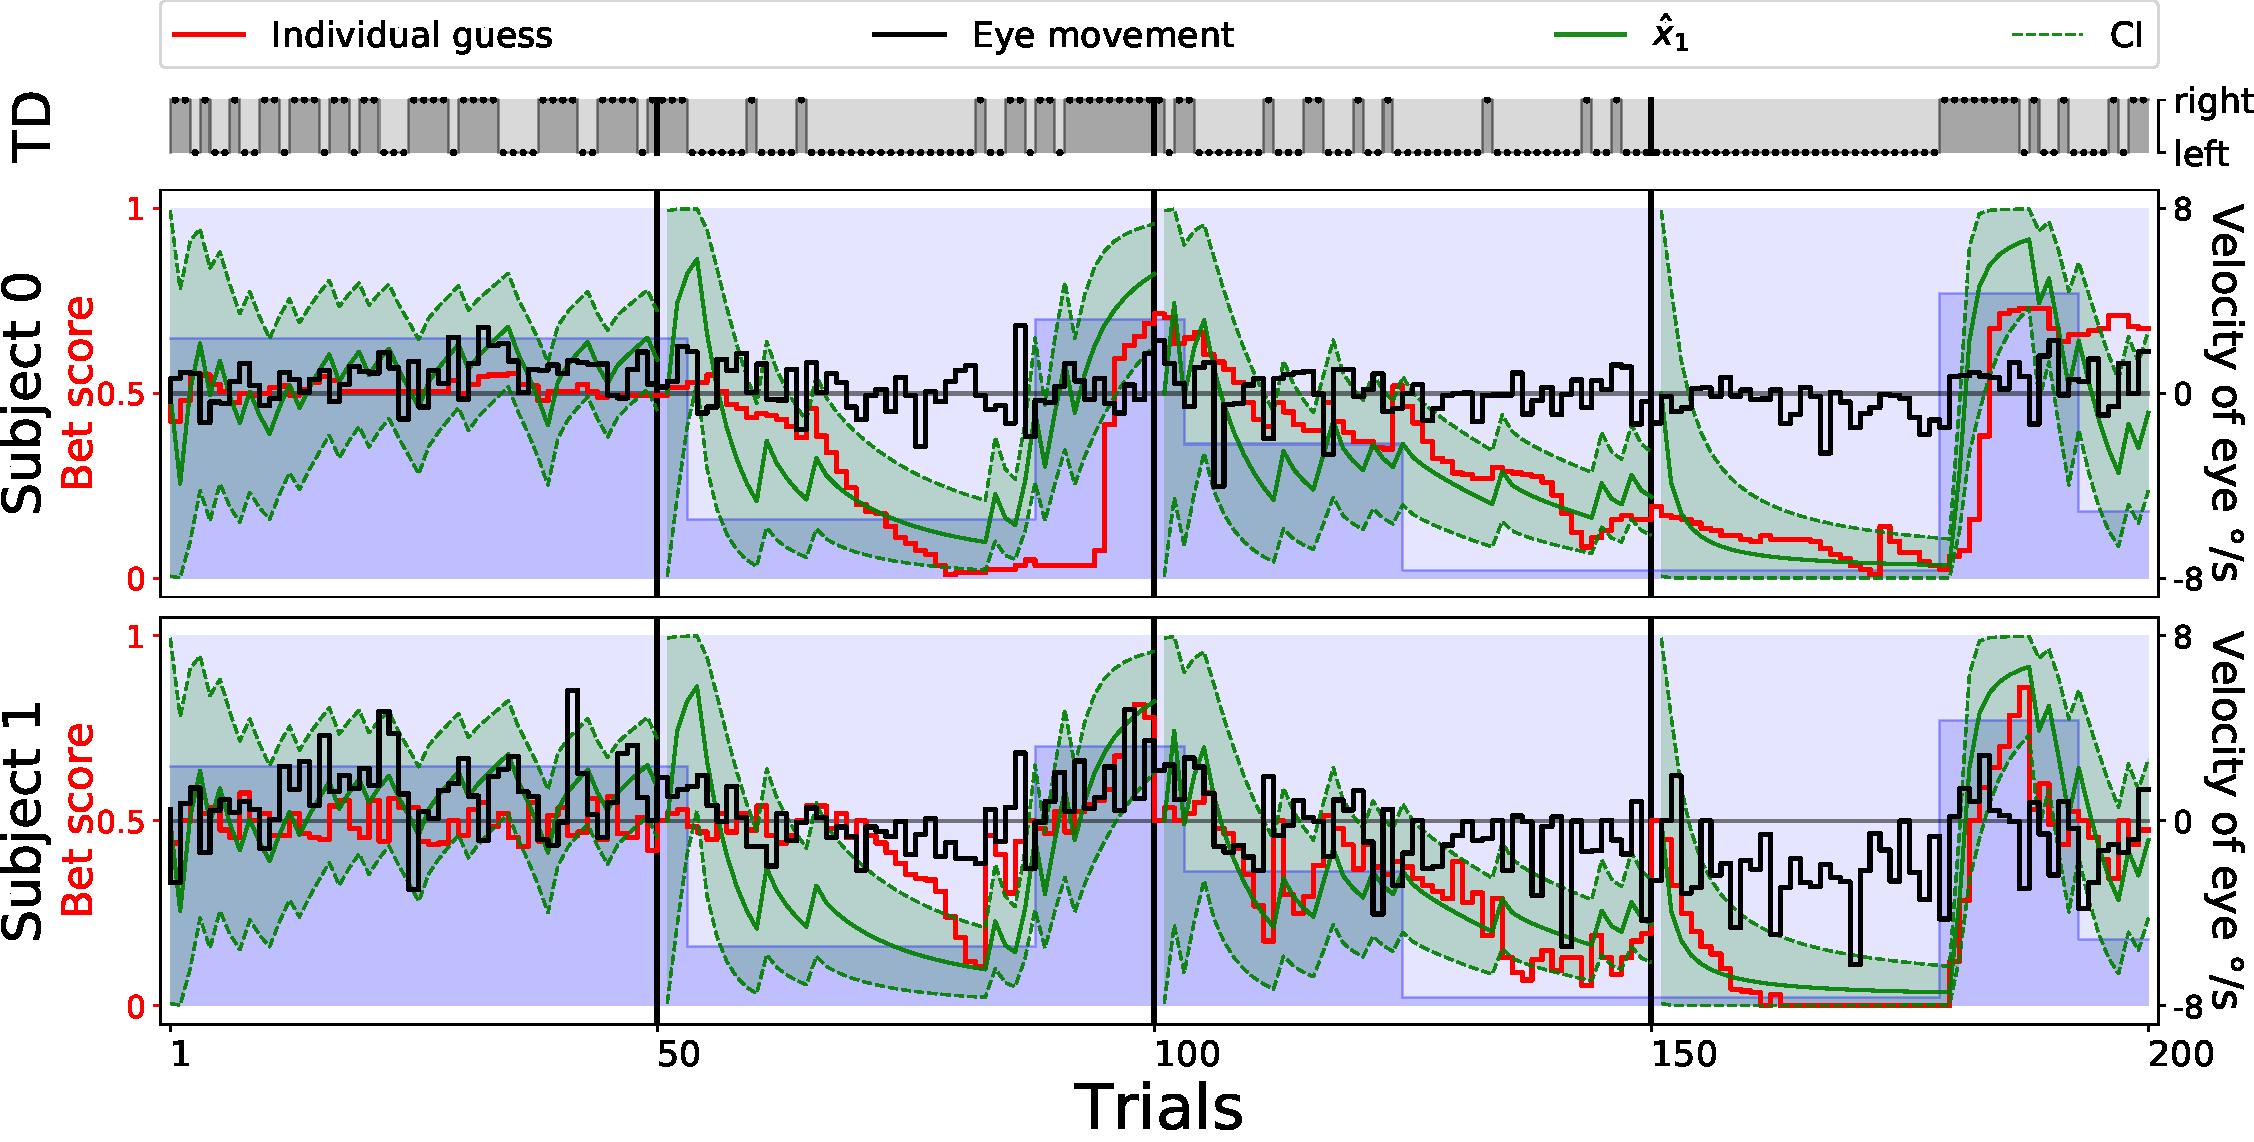
\includegraphics[width=\linewidth]{2_results_enregistrement}}
\caption{
\textbf{Behavioral results, qualitative overview.} %
For one trial block of $200$ trials, we compare the different model-estimated probabilities with respect to the behavioral results.
The top row represents the sequence of target directions (TD)
that were presented to observers and agents,
as generated by the binary switching model (see~\seeFig{intro}-A).
We show the evolution of the value
of the (true) probability bias $P_{\text{true}}$ (blue line)
which is hidden to observers
and that is used to generate the TD sequence above.
We have overlaid the results of
the probability bias predicted with a leaky integrator ($P_{\text{leaky}}$, orange line)
and with the BBCP model ($P_{\text{BBCP}}$, see~\seeFig{Bayesianchangepoint}-B, green line).
Bottom two rows display the raw behavioral results
for the $n=12$ observers, by showing their median (lines) and the .25 and .75 quantiles (shaded areas):
First, we show the  anticipatory pursuit eye velocity, as estimated right before
the onset of the visually-driven pursuit.
Below, we show the explicit ratings about the expected target direction (or \textit{bet scores}).
These plots show a good qualitative match between
the experimental evidence and the BBCP model,
in particular after the switches.
Note that short pauses occurred every $50$ trials
(as denoted by vertical black lines, see main text),
and we added the assumption in the model
that there was a switch at each pause.
This is reflected by the reset of the green curve close to the $0.5$ level and
the increase of the uncertainty after each pause. %multiple of $50$ trials.
}
\label{fig:results_psycho}
\end{figure}
%-------------------------------------------------------------%
%-------------------------------------------------------------%
%: 3A raw results in anticipatory pursuit
%-------------------------------------------------------------%
We used the binary switching model model to generate the (pseudo-)random sequence of
the target's directions (the alternation of leftward/rightward trials)
as the sequence of observations that were used in both sessions
(see~\seeFig{results_psycho}).
In the top panel  of~\seeFig{results_psycho}, we show the actual sequence of binary choices
(TD, leftward or rightward) of the Bernoulli trials.
In the panel below, we compare %the evolution of the recorded anticipatory pursuit (grey line) with
the true value of the hidden probability bias $x_1$ (step-like blue curve),
and the median predicted values using the leaky integrator ($P_{\text{leaky}}$, orange color) and BBCP model ($P_{\text{BBCP}}$, green color),
along with the $.05$ to $.95$ quantile range (green shaded area),
just as in~\seeFig{Bayesianchangepoint}-B.
In the middle panel of~\seeFig{results_psycho}, we show the median (with the $0.25$ ans $0.75$ quantiles) anticipatory pursuit velocity (for details see Materials and Methods in ~\seeSec{methods})
for the $12$ participants, throughout a trial block of $200$ trials of the experimental sequence.
% Note that these participants were chosen as those
% whose fitting score was nearest to the median score in the quantitative analysis
% that will be illustrated below in~\seeSec{inter}.
First, one can observe a trend in the polarity of anticipatory pursuit velocity
to be negative for probability bias values below~$.5$ and positive for values above~$.5$.
Comparing the raw anticipatory pursuit results with the BBCP agent predictions,
it appears qualitatively that both traces evolve in good agreement.
In particular, both curves unveil similar delays in detecting and
taking into account a switch of the probability bias (while being hidden to the observers),
reflecting the time (in the order of a few trials) taken to integrate enough information
to build up the estimation of a novel expectation about the probability bias value
which parameterizes this Bernoulli trial.
In general, results are more variable when the bias is weak ($p\approx .5$)
than when it is strong (close to zero or one),
consistent with the well-known dependence of the variance of a Bernoulli trial
upon the probability bias ($\textrm{Var}(p)= p \cdot (1-p)$).
In addition, the precision (i.e. the inverse of the variance)
of the inferred probability bias $\hat{x}_1$ increases
in longer epochs, as information is integrated over more trials.
As a result, the inferred probability as a function of time
seems qualitatively to constitute a reliable regressor
for predicting the amplitude of anticipatory pursuit velocity.

%-------------------------------------------------------------%
%: 3B Results: bias rating scale measurements
%-------------------------------------------------------------%
%\label{sec:rating_scale}
In addition, the explicit ratings
for the next trial's expected motion direction (or \textit{bet scores}, red curve in~\seeFig{results_psycho})
provided in the other experimental session
seem to qualitatively follow the same trend.
As with anticipatory pursuit, the series of the participants' bias guesses
exhibits a positive correlation with the true probability bias:
The next outcome of $x_{0}^{t}$ will in general be correctly inferred,
as compared to a random choice, as reported previously~\citep{Meyniel15}.
Indeed, similarly to the amplitude of anticipatory pursuit velocity,
we qualitatively compare in~\seeFig{results_psycho}
the trace of the bet scores
with the probability bias $\hat{x}_1$ inferred by the BBCP model.
Moreover, we observe again that a stronger probability bias leads
to a lower variability in the bet scores, compared to bias values close to $0.5$.
Again, a (hidden) switch in the value of the bias is
most of the time correctly identified after only a few trials.
Finally, note that after every pause (black vertical bar in~\seeFig{results_psycho}),
participants tended to favor unbiased guesses, closer to $0.5$.
We can speculate that this phenomenon could correspond
to a spontaneous resetting mechanism of the internal belief on the probability bias
and indeed, we can introduce such an assumption in the model
as a reset of the internal belief after each pause.
To conclude, the experiment performed in this session
shows that the probability bias values that are explicitly estimated by participants
are qualitatively similar to the implicit ones
which supposedly underlie the generation of graded anticipatory pursuit.

%-------------------------------------------------------------%
%: FIGURE 4  fig:results_psycho_all \seeFig{results_psycho_all}
\begin{figure}%[b!]
\centering{
\begin{tikzpicture}%[thick,scale=1, every node/.style={scale=1} ]
\node [anchor=north west]  (img4) at (0.000\linewidth,.618\linewidth){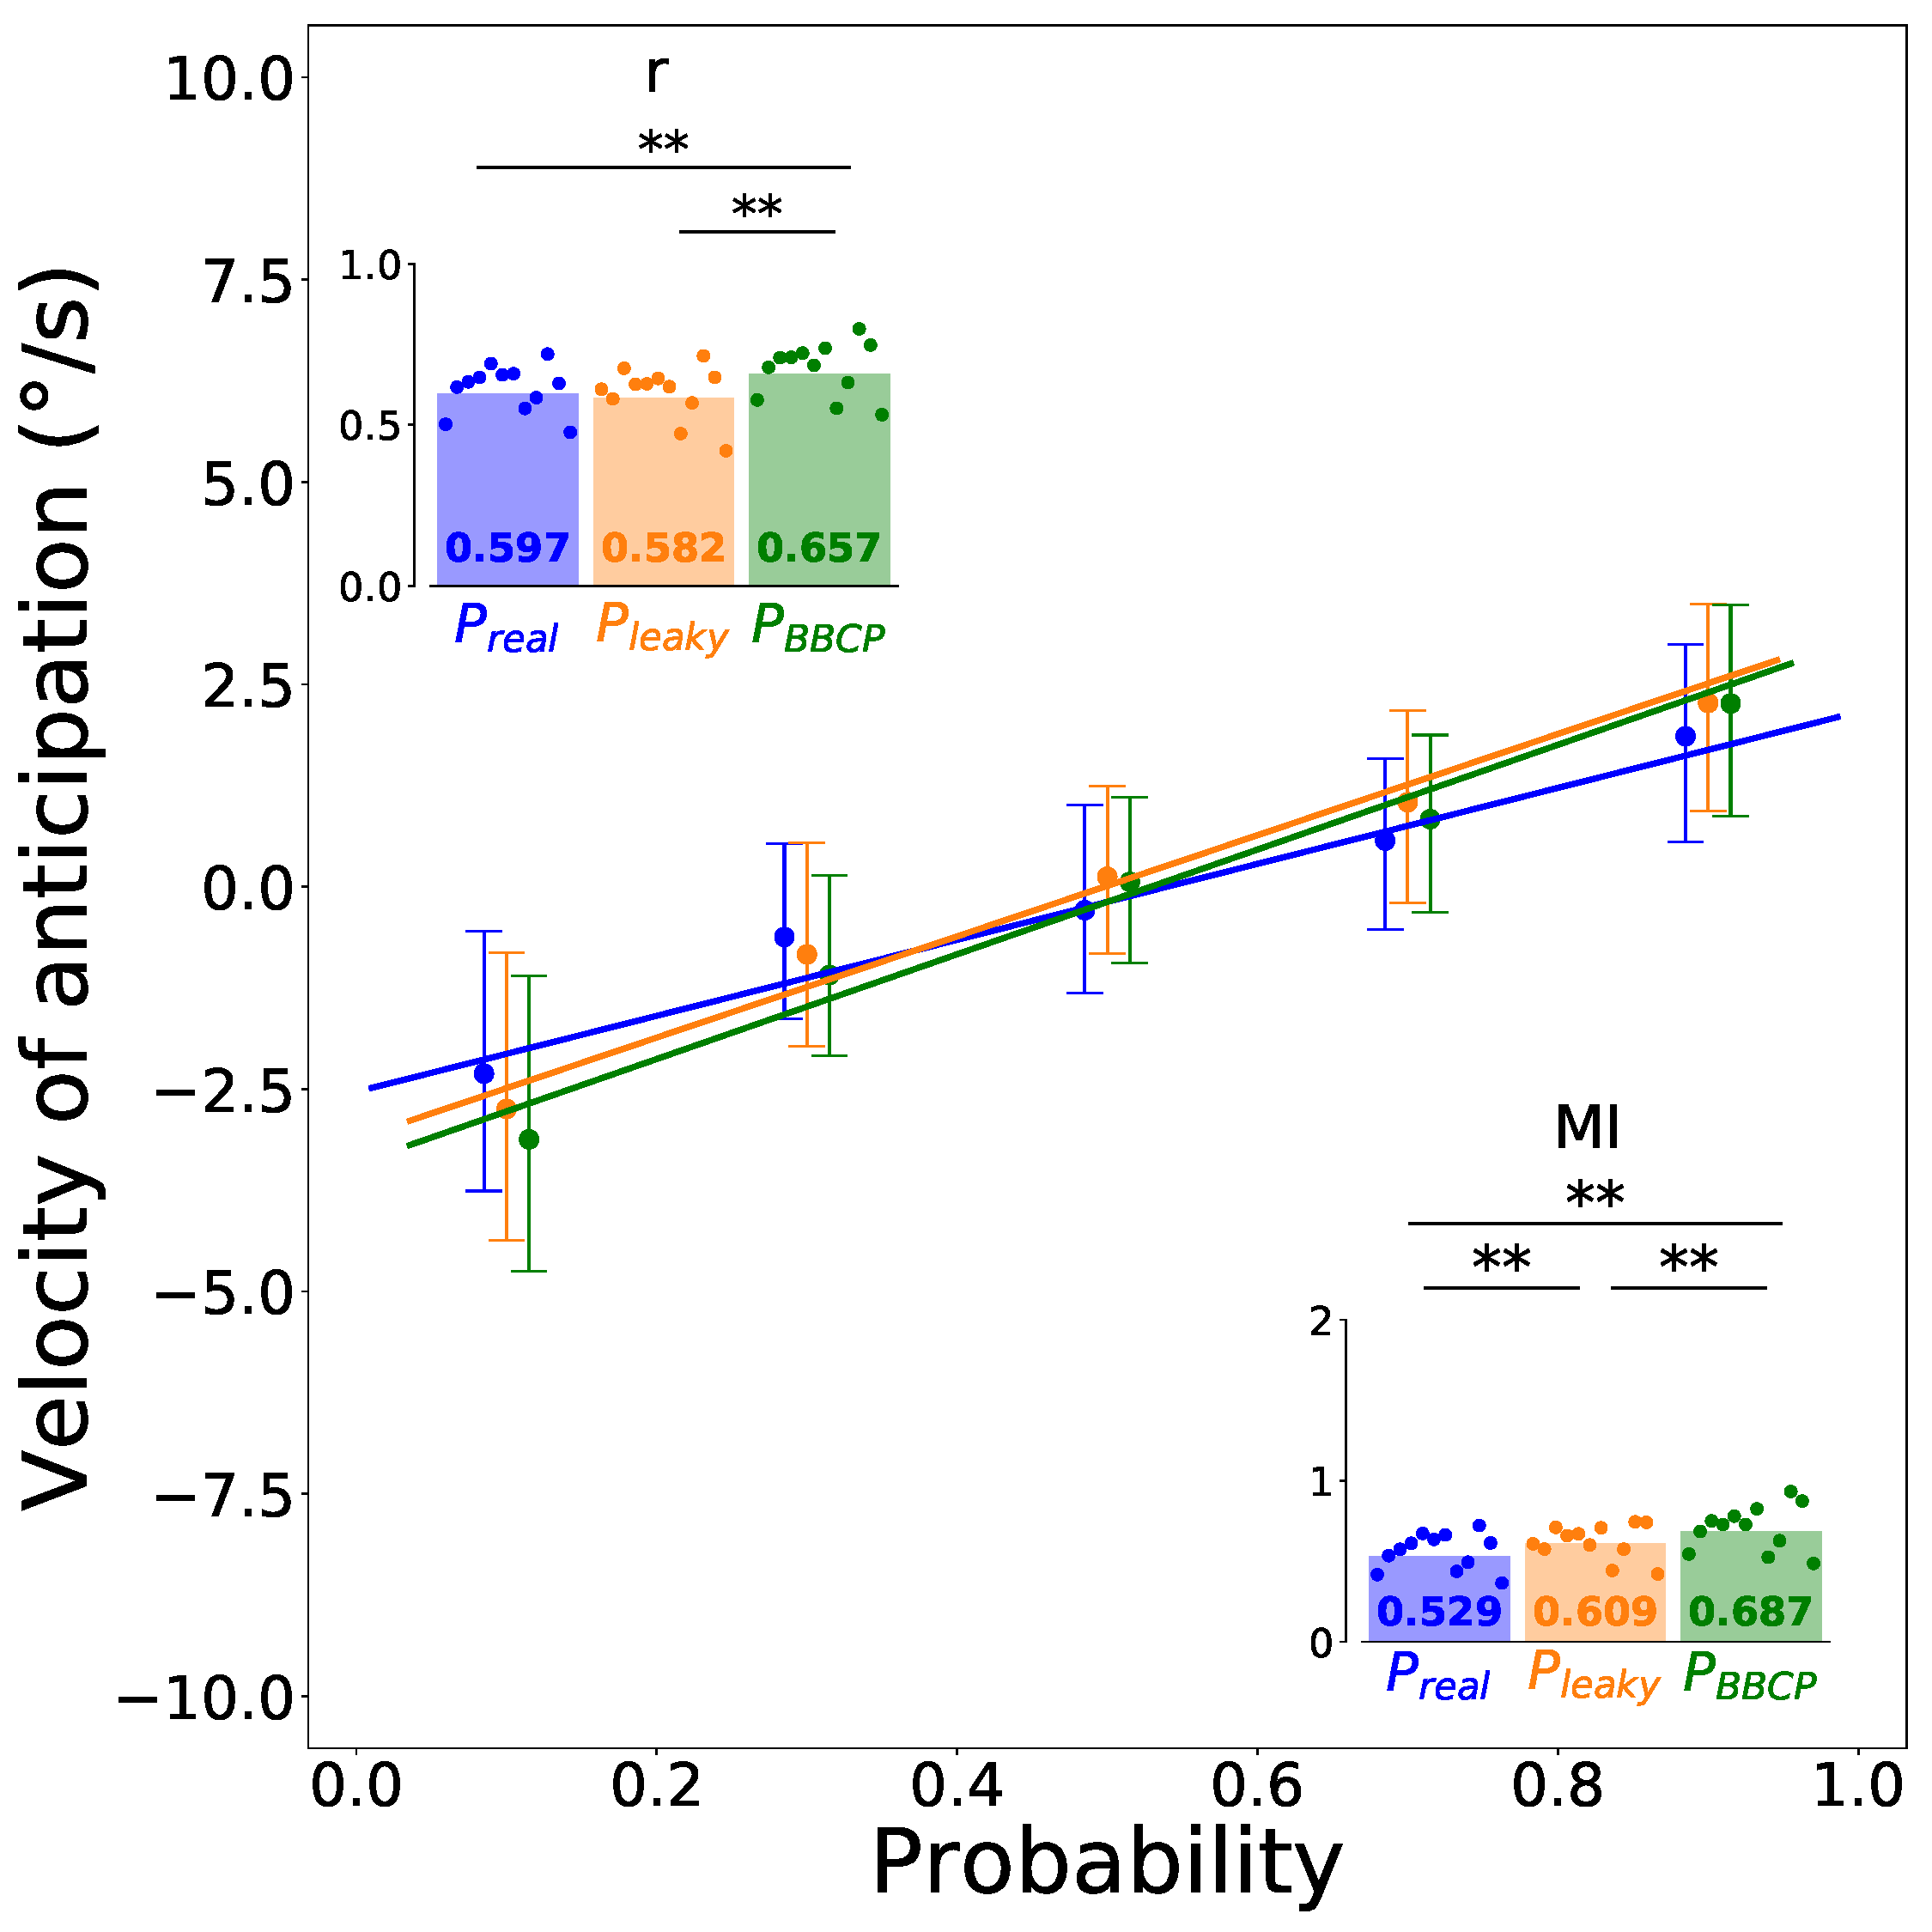
\includegraphics[width=0.49\linewidth]{4_A_result_psycho_aSPEM}};
\node [anchor=north west]  (img4) at (0.51\linewidth,.618\linewidth){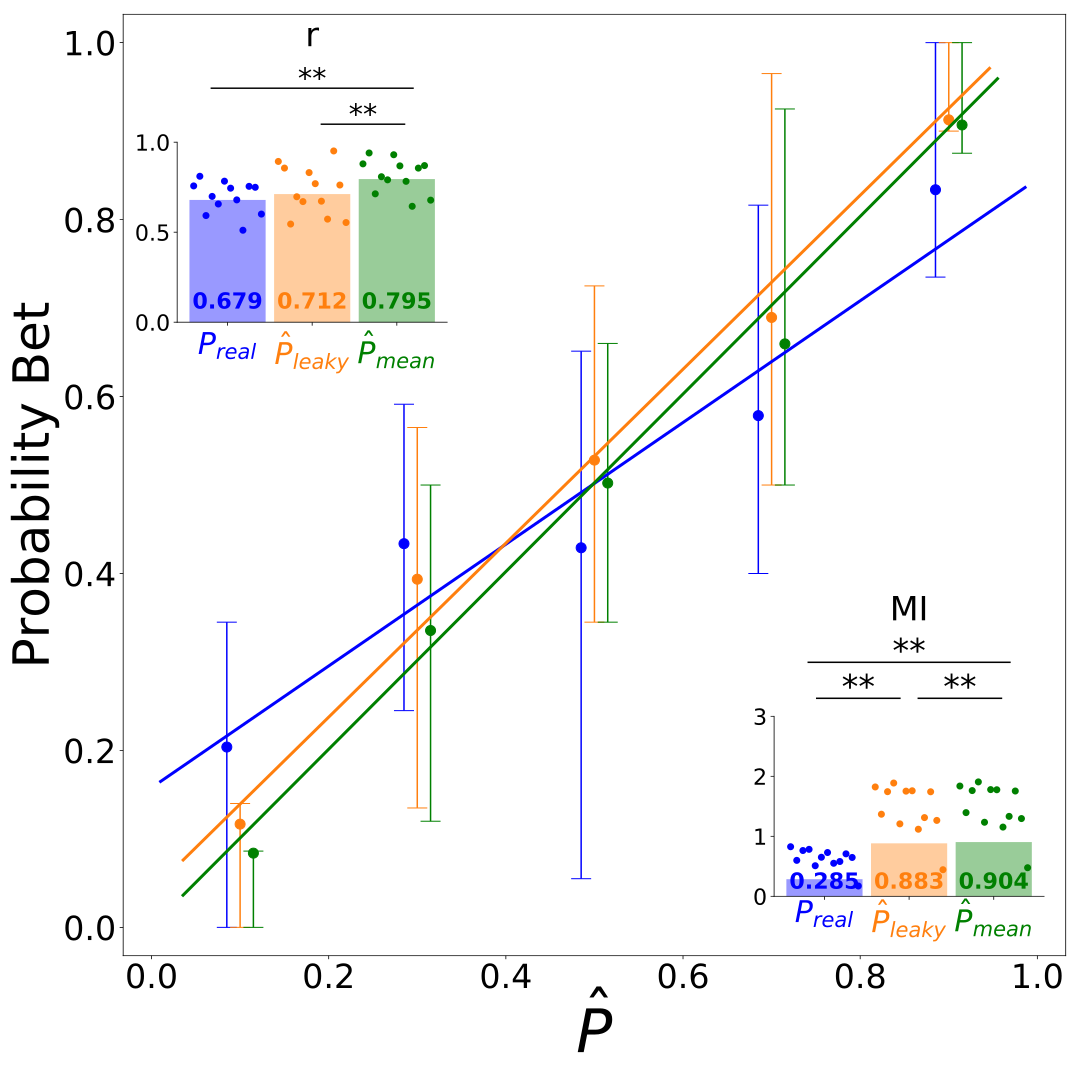
\includegraphics[width=0.49\linewidth]{4_B_result_psycho_bet}};
%
\draw [anchor=north west] (0.000\linewidth, .638\linewidth) node {$\mathsf{(A)}$};
\draw [anchor=north west] (0.5\linewidth, .638\linewidth) node {$\mathsf{(B)}$};
%
\end{tikzpicture}
}
\caption{%
\textbf{Behavioral results, quantitative analysis across participants ($n=12$).} %
% \Rone{Fig 4. An indication of n on the figure would be welcome (I assume it is n observers). "For all participants and for all trials" is an ambiguous description. Was it one estimate per participant, averaging all trials? or were all trials pooled together disregarding participants?}
To analyze the relation between these behavioral data with the predictions made by models,
we first looked at the variability of all these measures
conditioned on the predicted probability and
gathered over 5 equal partitions of the $[0, 1]$ probability segment.
For the $12$ participants, we collected an estimate of
\textit{(A)} the amplitude of anticipatory pursuit (aSPEM)
and \textit{(B)} the bet score value.
As a regressor, we have used the true probability ($P_{\text{true}}=x_1^t$, blue color),
and the probability bias estimates obtained with a leaky integrator ($P_{\text{leaky}}$, orange color)
and by the BBCP model ($P_{\text{BBCP}}$, green color).
We display these functional relations
using an error-bar plot showing the median with $.25$ and $.75$ quantiles
over the 5 partitions.
This shows a monotonous dependency for both behavioral measures with respect to the probability,
close to a linear regression, but with different strengths.
Second, we summarize in insets  quantitative measures of the strength of this dependence for each participant individually,
by computing the squared Pearson correlation coefficient $r^2$
and the mutual information (MI).
Dots correspond to these measures for each individual observer,
while the bar gives the median value over the population.
This confirms quantitatively that for both experimental measures,
there is a strong statistical dependency between
the behavioral results and the prediction of the BBCP model,
but also that this dependency is significantly stronger than that obtained
with the true probability and with the estimates obtained with the leaky integrator
(stars denote significative differences, see text for details).
}
\label{fig:results_psycho_all}
\end{figure}
%%-------------------------------------------------------------%
%-------------------------------------------------------------%
%: 3C quantitative analysis
%-------------------------------------------------------------%
Quantitatively, we now compare the experimental results
with the value of the probability bias $\hat{x}_1$
predicted by the leaky and BBCP algorithms.
Compiling results from all participants,
we have plotted in~\seeFig{results_psycho_all}
the anticipatory pursuit velocity (panel A) and the bet scores (panel B)
as a function of the predicted probability biases.
In a first analysis, all trials from all participants were pooled together
and we show this joint data as an error bar plot
as computed for 5 equal partitions of the $[0, 1]$ probability segment
showing the median along with the $.25$ and $.75$ quantiles.
As a comparison, the same method was applied to the true value $P_{\text{true}}$ and
to the estimate obtained by the leaky integrator  $P_{\text{leaky}}$.
We remind here that the true value of the probability bias
was coded at the second layer of the binary switching generative model and
is hidden both to the agents and to the human observers.
%
Qualitatively, as we can see in~\seeFig{results_psycho_all}-A,
the predicted probability bias
is linearly correlated with the anticipatory pursuit velocity
and this dependence is stronger with the
the probability bias predicted by the leaky and BBCP algorithms
(respectively $P_{\text{leaky}}$ and $P_{\text{BBCP}}$).
In a second analysis, we quantitatively estimated the squared Pearson correlation coefficient
and the mutual information
between the raw data and the different models, both as computed on the whole data or
for each observer individually (see insets in~\seeFig{results_psycho_all}).
The respective values for the whole dataset
($r^{2} = 0.486$ and $MI = 0.729$) and across participants
%notebook 4}
% ($r = 0.673 \pm 0.079$ and $MI =  0.707 \pm 0.134$)
($r^2 = 0.459 \pm 0.104$ and $MI = 0.707 \pm 0.134$)
are slightly higher than that found by~\citet{Montagnini2010} and~\citet{Damasse18}
for anticipatory pursuit measures gathered across experimental trial blocks with fixed direction biases %($r = XXX \pm $),
and significantly\footnote{All following $p$-values are obtained from the \href{https://docs.scipy.org/doc/scipy/reference/generated/scipy.stats.wilcoxon.html}{Wilcoxon signed-rank test}.} better than that estimated
with the true probability
% ($r = 0.613 \pm 0.069$ with $p=0.002$ and $MI = 0.562 \pm 0.107$ with $p=0.002$) %
($r^{2} = 0.381 \pm 0.083$ with $p=0.002$
and $MI = 0.562 \pm 0.107$ with $p=0.002$)
and for that estimated by the leaky-integrator model
% ($r = 0.600 \pm 0.079$ with $p=0.003$ and $MI =  0.622 \pm 0.102$ with $p=0.004$),
($r^{2} = 0.366 \pm 0.089$ with $p=0.002$ and $MI = 0.622 \pm 0.102$ with $p=0.004$)
see inset).

A similar analysis
illustrates the relationship between
the model-estimated probability bias
and the rating value, or bet score, about the expected outcome, which was provided at each trial
by participants
and is shown in~\seeFig{results_psycho}.
Similarly to the anticipatory pursuit velocity, the rating values are nicely correlated
with the probability bias given by the model,
as quantified by the squared Pearson correlation coefficient and mutual information
across participants ($r^{2} = 0.670 \pm 0.145$ and $MI = 1.312 \pm 0.364$).
Importantly, this value is again higher for the BBCP model than
for the leaky integrator ($r^{2} = 0.551 \pm 0.19$ with $p=0.018$ and $MI = 1.117 \pm 0.409$ with $p=0.028$),
or with the true probability ($r^{2} = 0.490 \pm 0.114$ with $p=0.002$ and $MI = 0.940 \pm 0.255$ with $p=0.002$).
Further notice that, in order to account for some specific changes
observed in the behavioral data after the short pauses
occurring every $50$ trials,
we added the assumption %for both models,
that there was a switch at each pause.
However, removing this assumption did not significantly change the conclusions about the match of the model
compared to $P_{\text{true}}$ or $P_{\text{leaky}}$
both for eye movements
($P_{\text{BBCP}}$: $r^{2} = 0.452 \pm 0.101$ and $MI =  0.712 \pm 0.125$,
$P_{\text{leaky}}$: $r^{2} = 0.305 \pm 0.077$ with $p=0.002$ and $MI =  0.577 \pm 0.096$ with $p=0.003$ ;
$P_{\text{true}}$ : $r^{2} = 0.381 \pm 0.083$ with $p=0.002$ and %
$MI =  0.562 \pm 0.107$ with $p=0.002$ )
and the bet experiment
($P_{\text{BBCP}}$: $r^{2} = 0.652 \pm 0.142$ and $MI =  1.255 \pm 0.349$, $P_{\text{leaky}}$: $r^{2} = 0.425 \pm 0.158$ with $p=0.002$ and $MI =  0.966 \pm 0.300$ with $p=0.002$ ; $P_{\text{true}}$ : $r^{2} = 0.490 \pm 0.114$ with $p=0.002$ and $MI =  0.940 \pm 0.255$ with $p=0.002$).
To conclude, we deduce that the dynamic estimate of the probability bias produced by the BBCP model
is a powerful regressor to explain
both the amplitude of anticipatory pursuit velocity
and the explicit ratings of human observers
experiencing a volatile context for visual motion.

%%%%%%%%%%%%%%%%%%%%%%%%%%%%%%%%%%%%%%%%%%%%%%%
\section{Results: Analyzing inter-individual differences}
%%%%%%%%%%%%%%%%%%%%%%%%%%%%%%%%%%%%%%%%%%%%%%%
\label{sec:inter}
%-------------------------------------------------------------%
%: 4A separate above analysis
%-------------------------------------------------------------%
So far, we have presented the qualitative behavior of individual participants and
have reported the quantitative analysis of the data
for the fit between experimental and model-inferred estimates of the hidden probability bias.
For instance, the experimental measures for the population of $12$ participants in~\seeFig{results_psycho},
support the qualitative match between behavioral data and model predictions,
which we then confirmed quantitatively on the whole group of participants.
It is important to note that no model fitting procedure was used so far,
but only the direct match of the prediction from the BBCP-model
resulting from the sequence of binary target directions
which were also presented to the human participants,
as shown in~\seeFig{Bayesianchangepoint}-B.
Nevertheless, we observed that in both sessions the qualitative match between model and data varied across participants.
This was best characterized by differences
in the variability of the responses, but also, for instance,
by the different characteristic delays after a switch.
This reflects the spectrum of individual behavioral choices
between exploitation versus exploration~\citep{Behrens07}.
As a consequence, we were interested in characterizing these individual preferences
for each individual participant,
and potentially to investigate whether this preference co-varied
across the two experimental sessions (i.e.~across implicit vs explicit response modalities).
Crucially, we have seen that the BBCP model is controlled by a single parameter,
the hazard rate, or equivalently by its inverse, the characteristic time~$\tau$.
Also, we have shown that knowing an observed sequence of behavioral responses,
we could fit the value of $h$ which would best explain the observations,
as quantified by the squared Pearson correlation coefficient or by the mutual information.
Thus, by extracting the best-fit parameters for each participant and experimental session,
we expect to better understand the variety of inter-individual differences. % and the covariation of these across response modalities.
%-------------------------------------------------------------%
%: FIGURE 5 fig:results_inter \seeFig{results_inter}
% cf https://github.com/laurentperrinet/Bayesianchangepoint/blob/master/notebooks/test_hazardrate.ipynb
% cf : 4_Meta_analysis.ipynb
\begin{figure}%[b!]
\centering{
\begin{tikzpicture}%[thick,scale=1, every node/.style={scale=1} ]
\node [anchor=north west]  (img4) at (0.000\linewidth,.57\linewidth){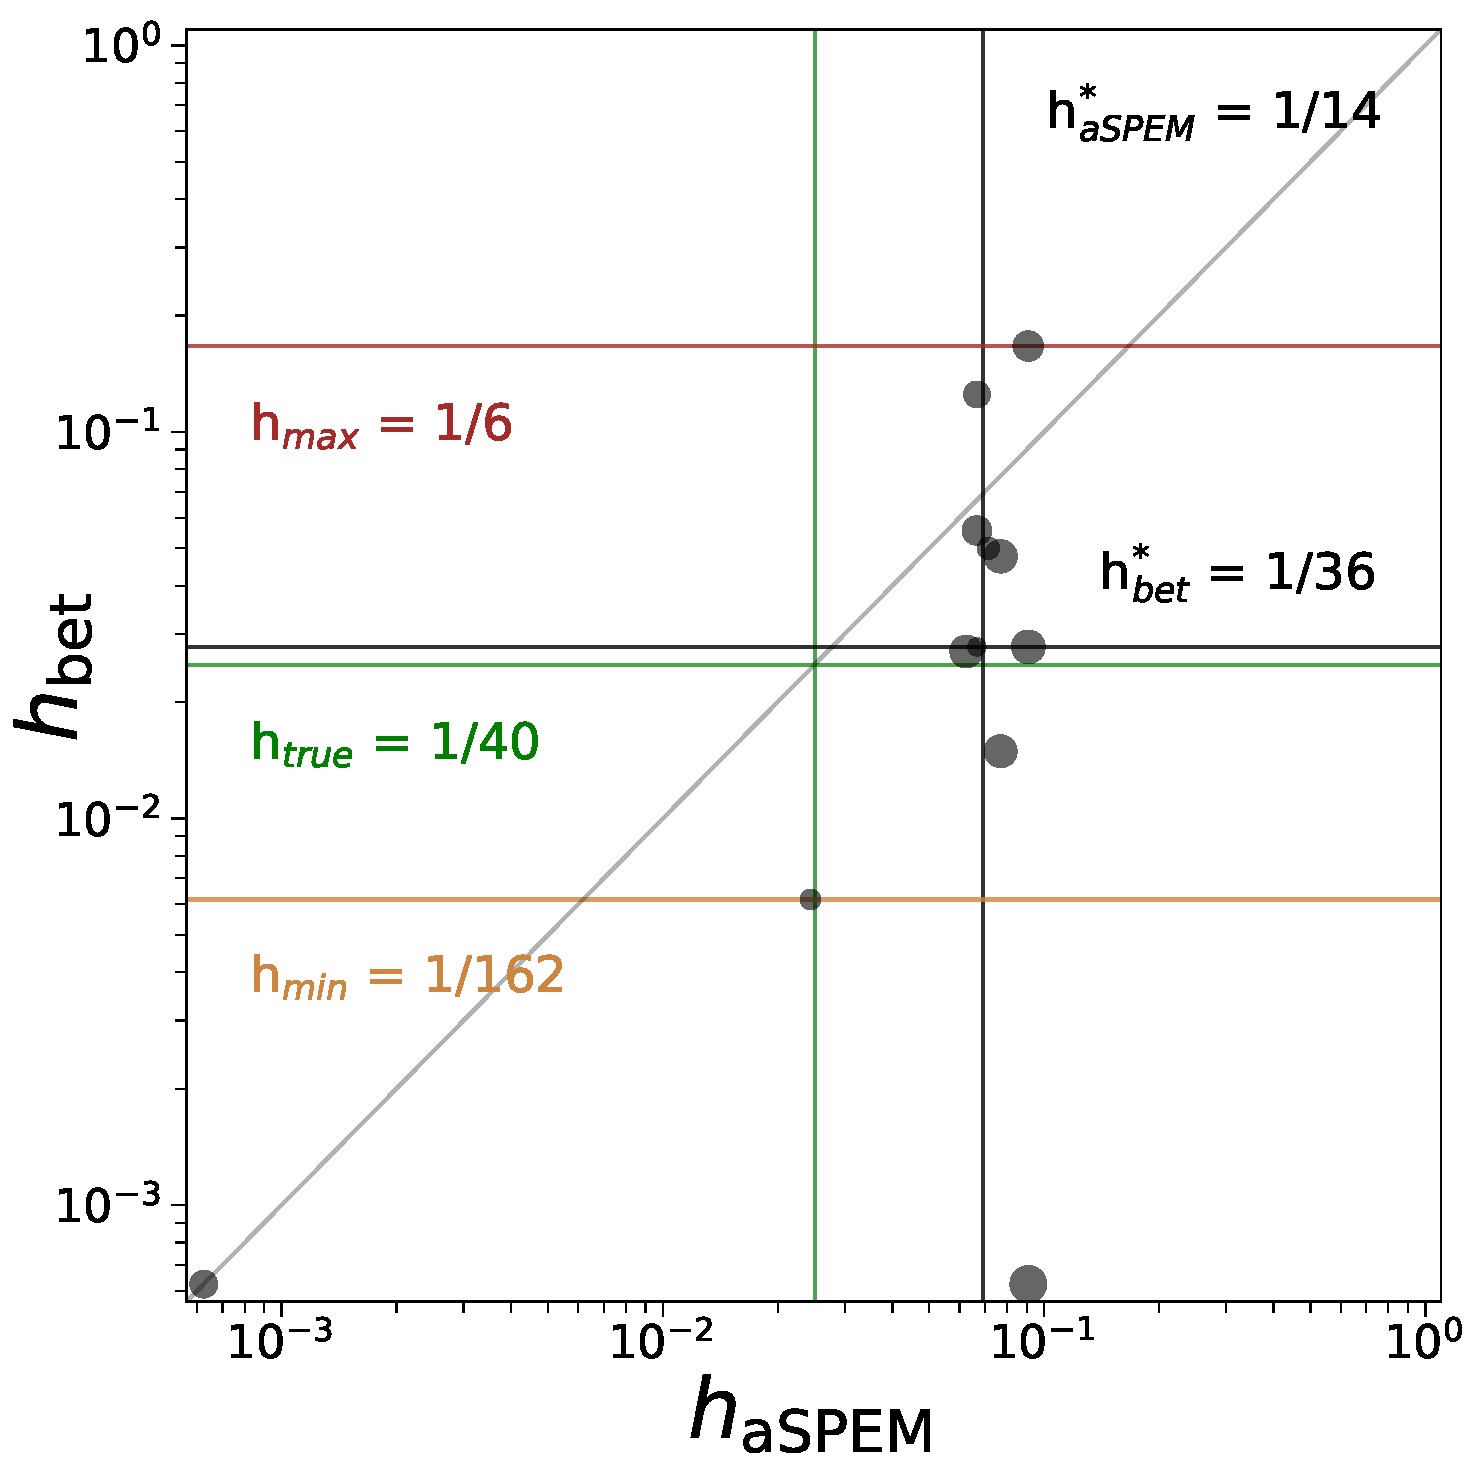
\includegraphics[width=0.38\linewidth]{5A_inter-individual_differences_fit}};
\node [anchor=north west]  (img4) at (0.4\linewidth,.59\linewidth){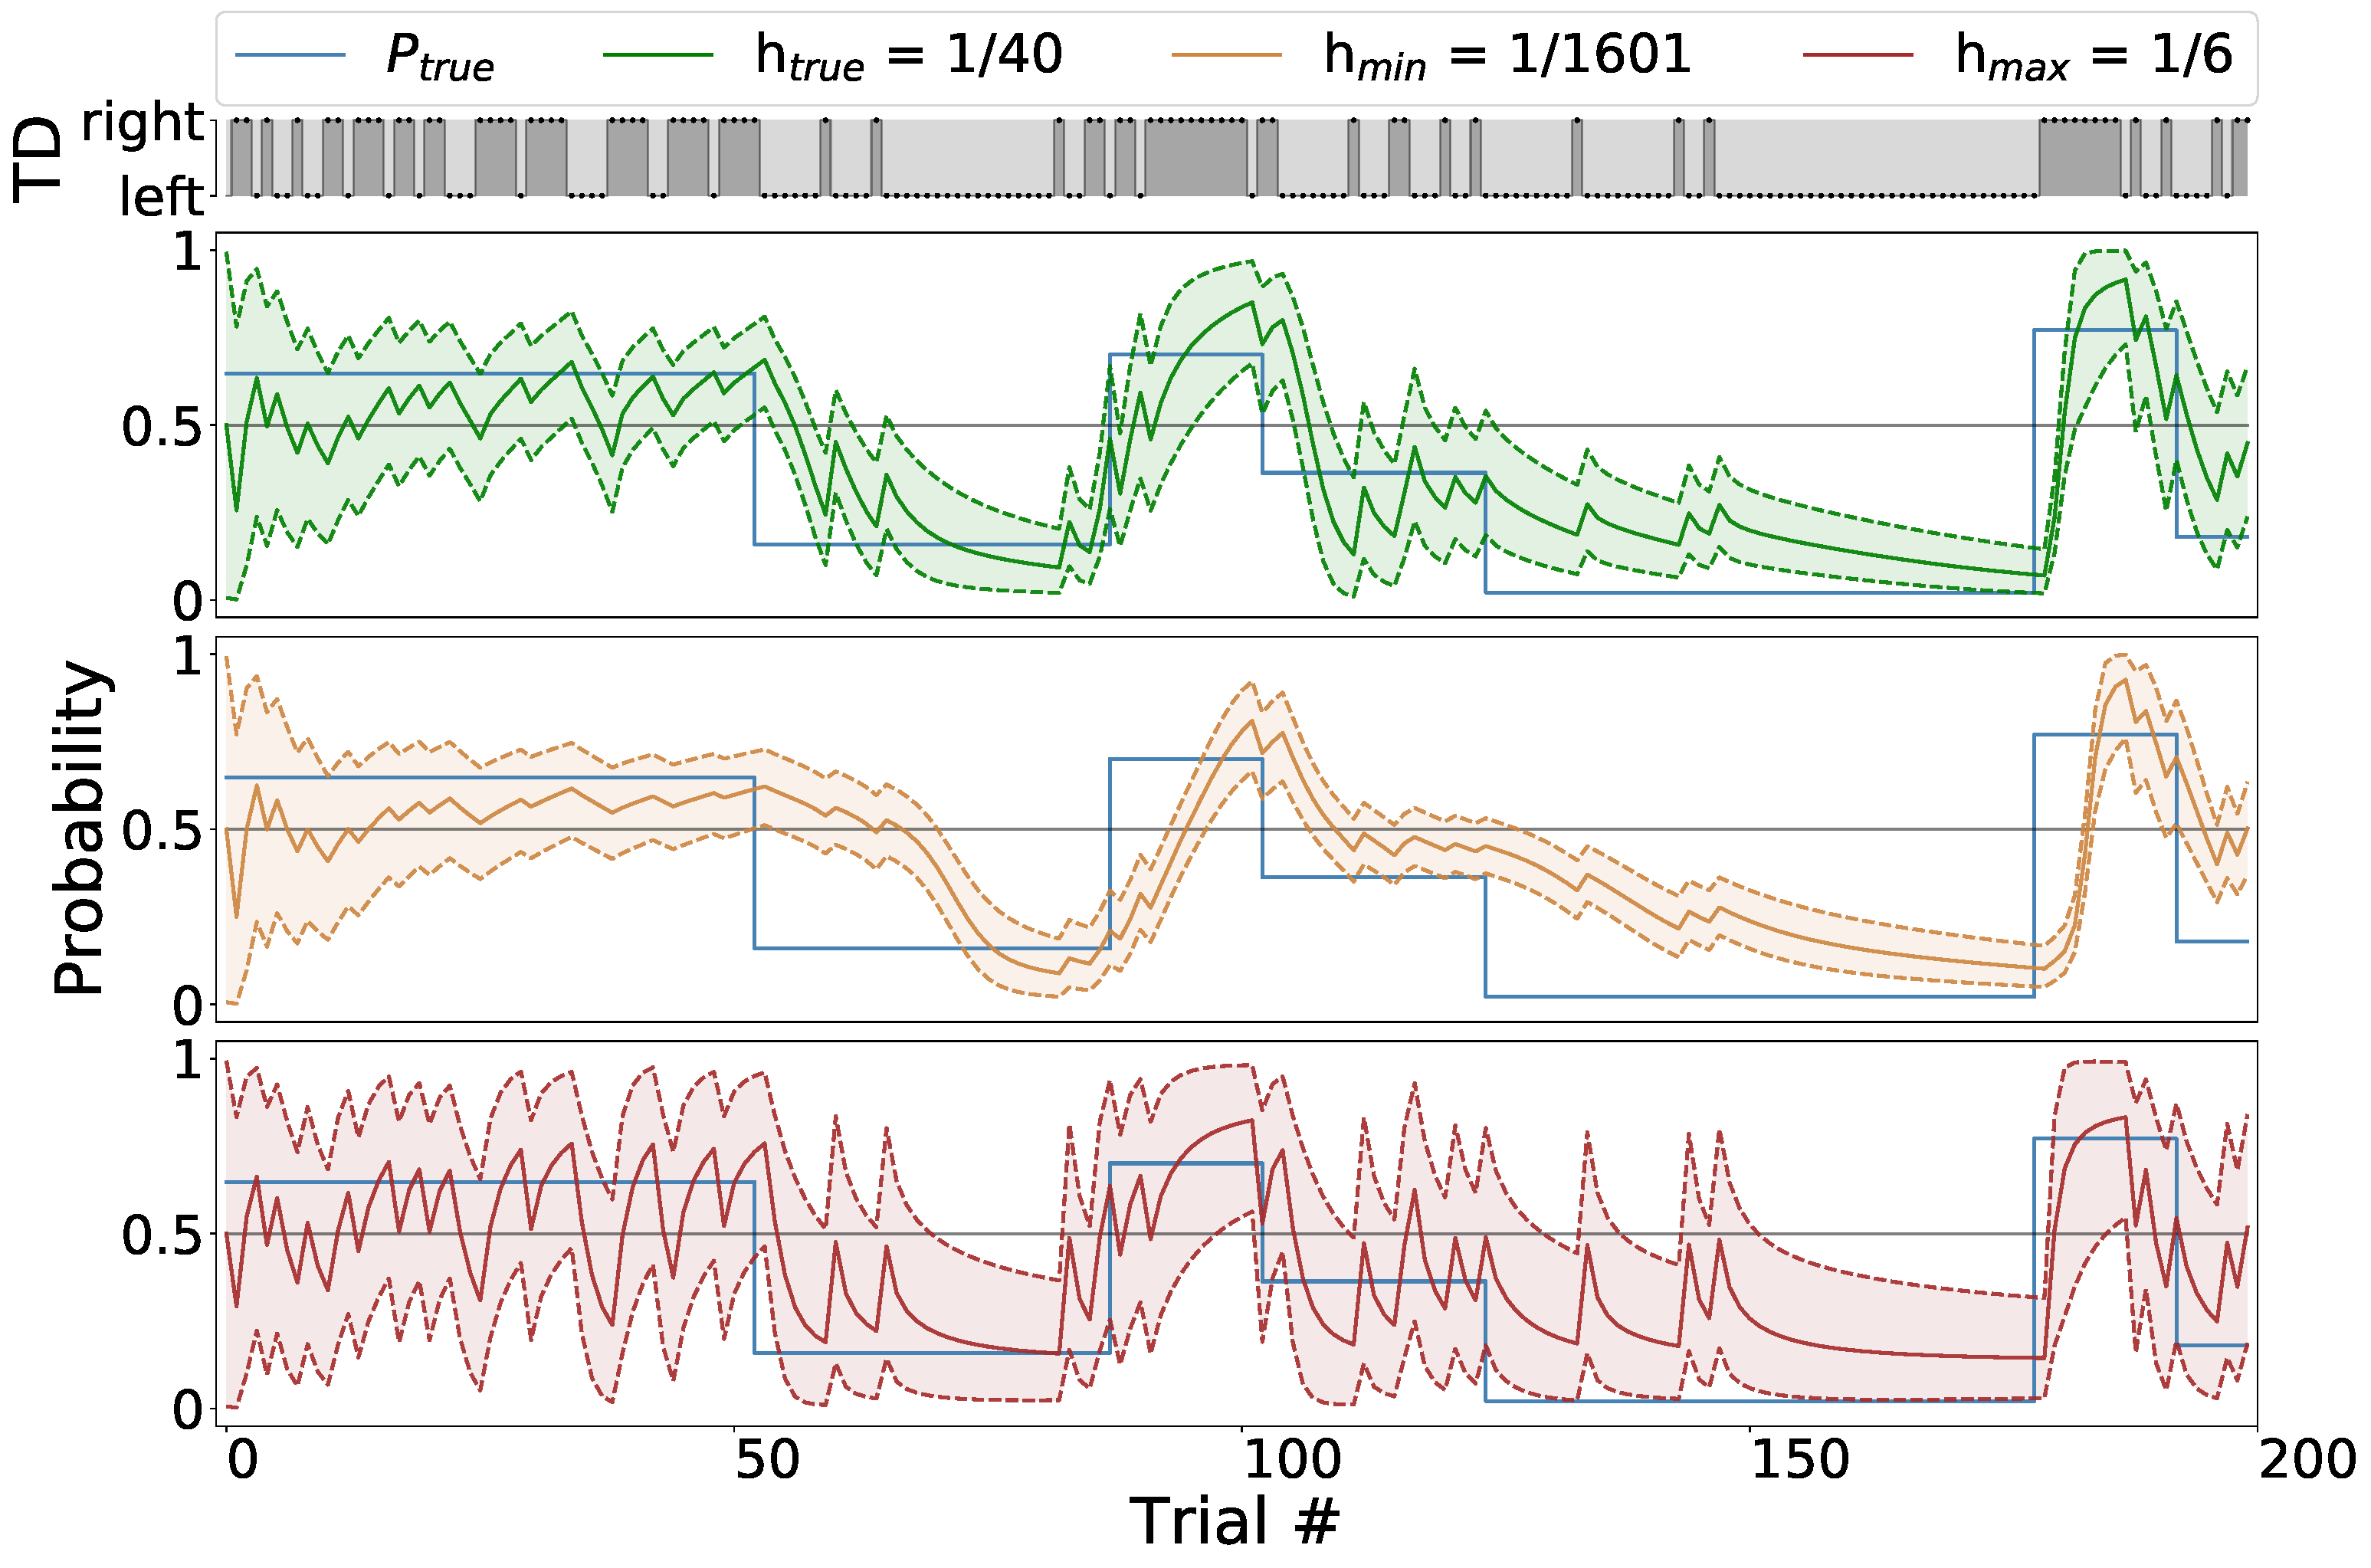
\includegraphics[width=0.58\linewidth]{5B_inter-individual_differences_fit}};
%
\draw [anchor=north west] (0.000\linewidth, .62\linewidth) node {$\mathsf{(A)}$};
\draw [anchor=north west] (0.4\linewidth, .62\linewidth) node {$\mathsf{(B)}$};
\end{tikzpicture}
}

%\centering{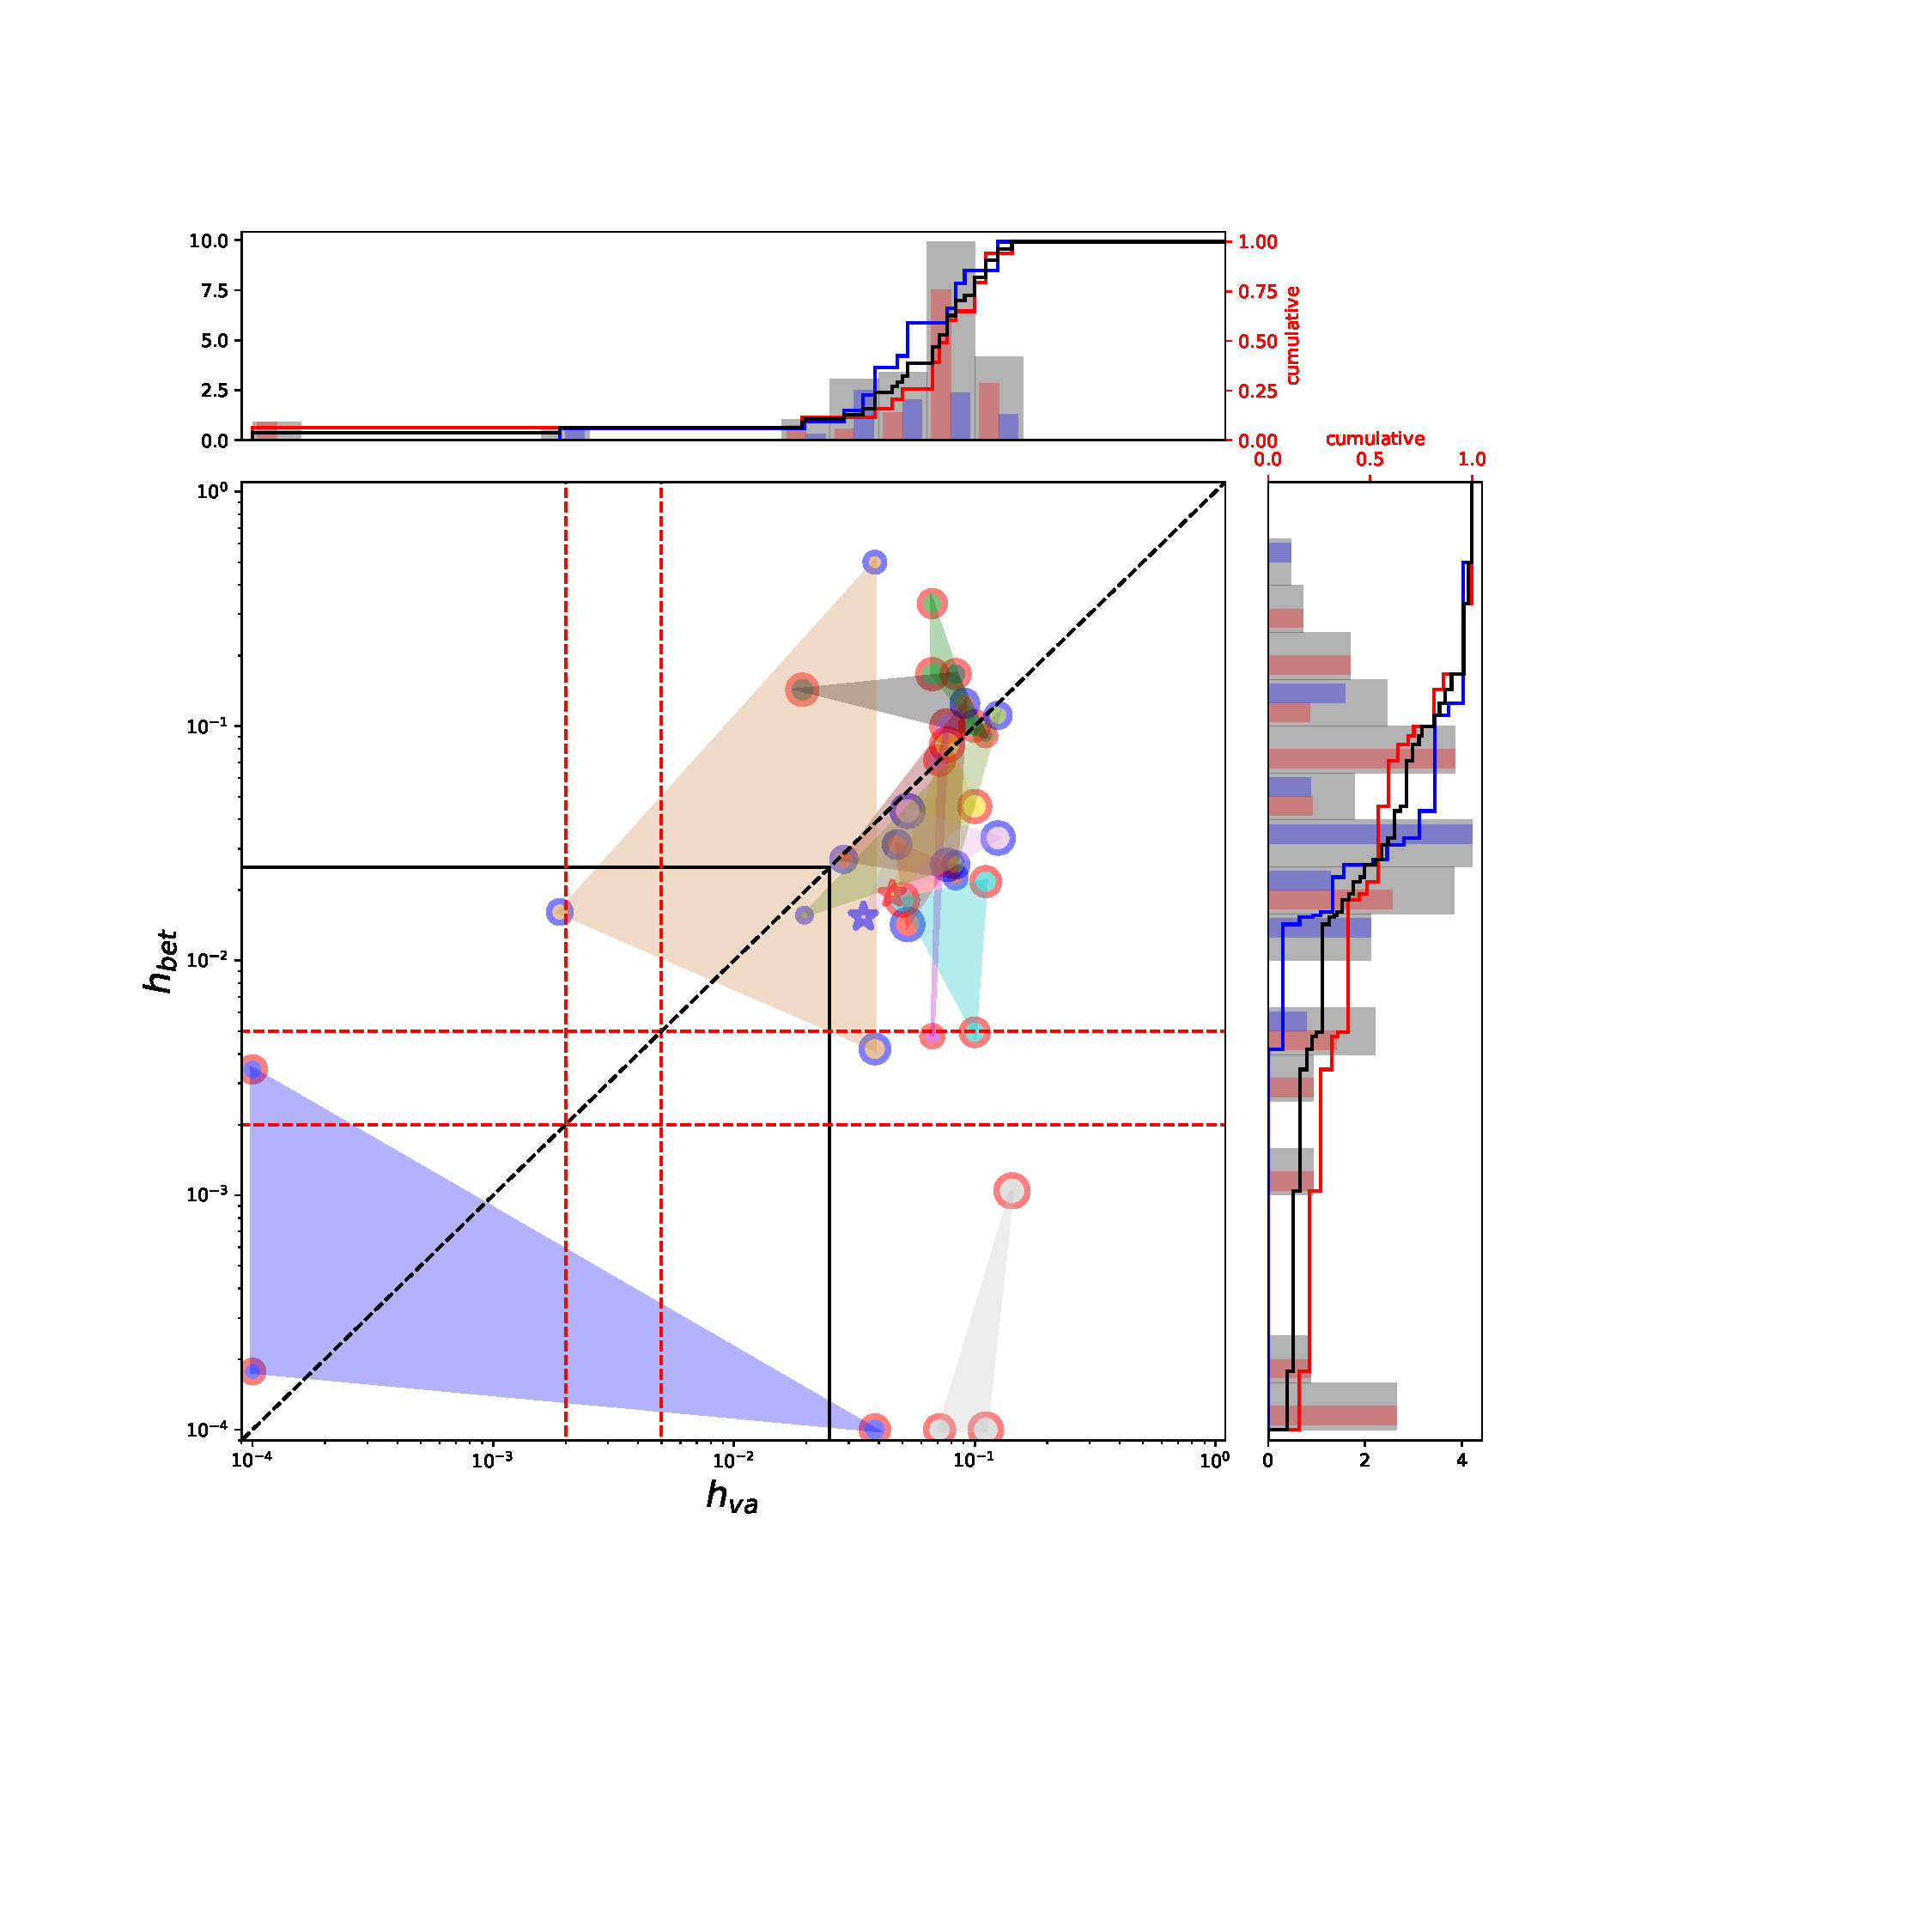
\includegraphics[width=0.618\linewidth]{5_inter-individual_differences_fit}}
\caption{\textbf{Analysis of inter-individual differences.} %
\textit{(A)}
We analyzed the behavior of the $n=12$ participants individually, by searching for each participant
the best value of the model's single free parameter, the hazard rate $h$.
Estimates were performed independently on both experiments,
such that we extracted different estimates of $h_{\text{aSPEM}}$ and $h_{\text{bet}}$
respectively for the anticipatory pursuit velocity and the rating value.
The dots correspond to independent estimates of the hazard rate
for each individual participant are shown as dots,
while the radius is proportional to the squared Person's correlation coefficient.
This plot shows that best fit hazard rates have a median value of  $h^{*}_{\text{aSPEM}}=\frac{1}{14}$ and $h^{*}_{\text{bet}}=\frac{1}{36}$.
The values are in general higher than the ground truth (blue line),
and in general higher for eye movements (below the diagonal).
Note that the dispersion of hazard-rate best-fit estimates is narrower
for the eye movement session than for the bet experiment.
Such an analysis may suggest that participants ultimately have
different mechanisms at the implicit (anticipatory pursuit) and explicit (ratings) levels
for guiding their tendency of exploitation versus exploration.
\textit{(B)} To illustrate the models corresponding to these best-fitted values of the hazard rates,
we show the predicted probability to the same sequence of TDs,
with the lowest ($\frac{1}{162}$), optimal ($\frac{1}{40}$) and highest ($\frac{1}{6}$) hazard rates
(respectively from top to bottom).
}
\label{fig:results_inter}
\end{figure}
%-------------------------------------------------------------%

%-------------------------------------------------------------%
%: 4B results
%-------------------------------------------------------------%
Hence, we have fitted the sequence of behavioral responses generated by each participant and
for each experimental session, with the predicted probability bias predicted by the BBCP model
with different values of its only free parameter, the hazard rate.
% that is, for the eye movements and the rating scale experiments.
To avoid any possible bias from the fitting procedure,
we tested $1600$ linearly spaced values of $\tau$ from $1$ to $1600$ trials.
For each, we computed the correlation coefficient with the responses of the BBCP model parameterized
by the value of the hazard rate $h = \frac 1 \tau$.
We then extracted different estimates of $h_{\text{aSPEM}}$ and $h_{\text{bet}}$,
respectively for anticipatory pursuit and the rating scale,
by choosing the hazard rate value corresponding to that with maximal correlation coefficient.
%To cross-validate our results for each individual participant,
%we have fitted the BBCP model to each of the $3$ trial blocks of $200$ trials.
%This provides with $3$ values of the best fitted hazard rate for each session and observer.
The scatter plot of the best fit values for each individual is shown in~\seeFig{results_inter}.
This figure suggests, in the first place, that there is some variability
in the best fitted value of the hazard rate in both sessions.
Overall, the value of correlation coefficient of the best fit hazard rate
was slightly higher than that computed in~\seeFig{results_psycho}
with $r^{2} = 0.471 \pm 0.109$ for the eye movement session
%$\text{MI} = XX~ \pm XX~$
%\CP{$h_{va}$: un r par sujet : $0.6826033619391142 \pm 0.08006027539364491$ //
%un MI par sujet : $ 0.479930369669249 \pm 0.12328555167152054$ //
%moyenne de tous les r trouv\'e : $0.639744367840892 \pm 0.11445851404708901$
%quand on prend un r par sujet il semble que ce soit un peut plus grand que quand on garde un h fixe, pas pour le MI ni pour quand on calcule la moyenne des 3 r par sujet (notebook 5)}
 and $r^{2} = 0.691 \pm 0.152$ for the rating scale session.
%$\text{MI} = XX \pm XX$
%\CP{$h_{bet}$ un r par sujet : $0.8117056662563028 \pm 0.08911550300859927$ //
%un MI par sujet :$0.8341219853735895 \pm 0.25926861033243437$ //
%moyenne de tous les r trouv\'e : $0.7975617439810163 \pm 0.14310508337570083$
%il semble que se soit moin bon que quand on garde un h fixe} for the second.
A part of the variability in the estimated hazard rates comes
from the limited length of the data blocks,
while another part is due to intra-individual and inter-individual variabilities.
Overall, the median (with $25\%$ and $75\%$ quantiles) are $h_{\text{aSPEM}} = 0.069 ~ (0.065, 0.080)$ %\CP{moyenne : $0.06692999125125686 \pm 0.03628253053391533$, mediane : 0.06904761904761905 	25\% 0.038461538461538464 	75\% 0.09318181818181817}
for the anticipatory pursuit session and
$h_{\text{bet}} = 0.027 ~ (0.012, 0.051)$ %\CP{moyenne : $0.06631464647744617 \pm 0.09970025861060718$, mediane : 0.02564102564102564 	25\% 0.011951909476661951 	75\% 0.09318181818181817
%}
for the rating scale.
We observe that these values are close to the (hidden) ground truth value ($h=1/40=0.025$) used to generate the sequence.
In addition, the best-fit hazard rate value is higher for anticipatory pursuit compared to the true value and the rating scale measures.
%Quantitatively, the ratio of both hazard rates computed across participants was \CP{with a ratio $1.6460031261743702~ \pm 2.779003512890947~$ ($h_{bet} / h_{va}$),  $16.12429536779007~ \pm 40.37883398426319~$ ($h_{va} / h_{bet}$)},
% In addition, we observed a tendency for hazard rate to be higher in the eye movement recording session.
%as was previously suggested~\citep{Meyniel??}.
%Importantly, there is a part of the variability
%which seems characteristic of the spectrum of individual choices.
%\LP{
%Indeed, each cluster of individual measures is qualitatively well separated and
%a simple k-means cluster analysis proves that
%given a couple of hazard rate values chosen at random,
%one could identify the participant with an accuracy of $XX\%$.
%As a comparison, the same analysis done based on the leaky integrator predictions
%showed that such accuracy would drop to $XX\%$,
%close to the chance level of $8.33\%$.
%} \CP{n'a pas fonctionn\'e !}
As an interim summary, this analysis reveals
that relaxing the free parameter of the BBCP model
improves the match of the model to the behavioral data, and that individual best-fitting hazard-rates are variable, especially for the Bet task.
% and that we could represent the distribution of individual differences in the choice behavior between exploration and exploitation in both sessions for each participant
Future work might provide important insight about the analysis of these inter-individual differences in terms of each participant's preference for exploration versus exploitation across different cognitive tasks.

%-------------------------------------------------------------%
%: 4C analysis
%-------------------------------------------------------------%
The distribution of best-fitted values for each individual participant seemed to qualitatively cluster,
but the dataset is still insufficiently large to support the significance of such observation
at a quantitative level.
Moreover, there is a difference in the distribution of observed hazard rates in both experiments.
Indeed, we observed that the marginal distribution for each session is different,
with the distribution in the anticipatory pursuit session being narrower than
that observed for the rating scale session.
In particular, we also observed the same behavior for each trial block independently,
suggesting that the origin of this variability mainly comes from inter-individual variability.
Second, there is an apparent lack of correlation between the explicit and the implicit estimates of the hazard rate,
yet we would need more empirical evidence to prove
that this originates from the experimental setup or rather by separate processing of volatility.
Such an analysis would suggest that even though the predictive processes
at work in both sessions may reflect a common origin for the evaluation of volatility,
this estimation is then more strongly modulated by individual preferences
when a more explicit cognitive process is at stake.
%%%%%%%%%%%%%%%%%%%%%%%%%%%%%%%%%%%%%%%%%%%%%%%%%%%%%%%%%%%%%%%
%: %%%%%%%%%%%%%%%%%%%%%%%%%%%%%%%%%%%%%%%%%%%%%%%%%%%%%%%%%%%%%%%
\section{Discussion}
%%%%%%%%%%%%%%%%%%%%%%%%%%%%%%%%%%%%%%%%%%%%%%%%%%%%%%%%%%%%%%%
\label{sec:outro}
%%%%%%%%%%%%%%%%%%%%%%%%%%%%%%%%%%%%%%%%%%%%%%%%%%%%%%%%%%%%%%%

The capacity to adapt our behavior to the environmental regularities has been investigated in different research fields, from motor priming and sensory adaptation to reinforcement learning, machine learning and economics. Several studies have aimed at characterizing the typical time scale over which such adaptation occurs. However, the pattern of environmental regularities could very well change in time, thereby making a fixed time-scale for adaptation a suboptimal cognitive strategy. In addition, different behaviors are submitted to different constraints and respond to different challenges, thus it is reasonable to expect some differences in the way (and time scales) they adapt to the changing environment. This study is an attempt to address these crucial open questions. We have taken an original approach, by assuming a theoretically-defined volatility in the properties of the environment (in the specific context of visual motion tracking) and we have developed an optimal inferential agent, which best captures the hidden properties of the generative model solely based on the trial sequence of target motion. We have then compared the optimal agent's prediction, as well as a more classical \textit{forgetful} agent, to two sets of behavioral data, one rooted in the early oculomotor network underlying anticipatory  tracking, and the other related to the explicit estimate of the likelihood of a future event. Our results point to a flexible adaptation strategy in humans, taking into account the volatility of the environmental statistics. The time-scale of this dynamic adaptive process would thus vary across time, but it would also be modulated by the specific behavioral task and by inter-individual differences. In this section we discuss the present work and its implications in view of the existing literature and some general open questions.

%\subsection{Environmental regularities, cognitive properties and visual perception}
% \AM{
\subsection{Measuring adaptation to volatile environments}
%}
The time-varying statistical regularities that characterize the environment are likely to influence several cognitive functions. In this study, we have made the choice to focus on a simple and probably mostly unconscious motor behavior (anticipatory pursuit), as well as on the explicit rating of expectation for the forthcoming motion direction. In contrast, we have not addressed the question of whether and how statistical learning affects visual motion perception throughout our model-generated volatile sequences. In an empirical context similar to ours, Maus et al~\citet{Maus2015} have recently shown that perceptual adaptation for speed estimation occurs concurrently to priming-based anticipatory pursuit throughout a sequence of motion tracking trials with randomly varying speed. They actually found a robust \emph{repulsive} adaptation effect, with perceptual judgements biased in favor of faster percepts after seeing stimuli that were slower and~\textit{vice-versa}. Concurrently, these authors also found a positive effect on anticipatory pursuit, with faster anticipation after faster stimuli, somehow in agreement with the adaptive properties of anticipatory pursuit that we report here. Moreover, they quantified the trial-history effects on anticipatory pursuit and speed perception by fitting a fixed-size memory model similar to our forgetful agent. They found that anticipatory pursuit and speed perception change over different time scales, with the priming effects being maximized for short-term stimulus history (around $2$ trials) and adaptation for longer stimulus history, around $15$ trials. Their main conclusion was that perceptual adaptation and oculomotor priming are the result of two distinct readout processes using the same internal representation of motion regularities. Note that both these history lengths can be considered short in comparison to the several hundreds of trials that are commonly used in psychophysics and sensorimotor adaptation studies and that, similar to the present study, the inferred characteristic times are even shorter for the buildup of anticipatory eye movements. However, it is also important to note that in the study by Maus et al~\citet{Maus2015}, the generative model underlying the random sequence of motion trials was different and much simpler than in the present study: In particular the role of environmental volatility was not directly addressed there. This makes a direct comparison between their results and ours difficult beyond a qualitative level.

In spite of a multitude of existing studies investigating the dynamics of sequential effects on visual perception (see for example~\citet{Cicchini_PRSB_2018,ChopinMamassian2012}), only few of them have directly addressed the role of the environmental volatility on the different behavioral outcomes. Meyniel et al~\citet{Meyniel16} have compared the predictions of different models, featuring a dynamic adaptation to the environment's volatility (equivalent to our \textit{forgetful agent model}) versus a fixed belief model, on five sets of previously acquired data, including reaction time, explicit reports and neurophysiological measures. Interestingly, they concluded that the estimation of a time-varying transition probability matrix constitutes a core building block of sequence knowledge in the brain,
which then applies to a variety of sensory modalities and experimental situations. Consequently, sequential effects in binary sequences would be better explained by learning and updating transition probabilities compared to the absolute item frequencies (as in the present work) or the frequencies of their alternations. The critical difference lies in the content of what is learned (transition probabilities versus item frequencies) in an attempt to capture human behavior. Rather than on transition probabilities, here we focused on the analysis and modeling of human behavior as a function of the frequency of presentation (and its fluctuations in time) of a given event in a binary sequence of alternating visual motion direction. We can speculate that different statistics can play different roles depending on the context, but altogether the study by Meyniel et al~\citet{Meyniel16} and the present one converge to highlight the importance of a dynamic estimate of the hierarchical statistical properties of the environment for efficient behavior. There are also other limits to the agent that we have defined. In this study, we assume that data is provided as a sequence of discrete steps. A similar approach using a Poisson point process
allows to extend our model to the continuous time domain, such as addressed by Radillo et al~\citet{RadilloBrady2017}: In their experiments, the authors analyzed the licking behavior of rats in a dynamic environment. The generalization to the time-continuous case is beyond the scope of our current protocol, but it would consist in a natural extension of it to more complex and ecological settings.

Our results demonstrate that the BCCP model is relatively good in mimicking the adaptive changes of both (implicit) anticipatory eye movements and (explicit) ratings of direction expectation in a volatile context. However, these two different behavioral measures, the implicit and the explicit one, are not correlated across individuals. This observation is certainly worth deeper investigation in the future as it raises doubts on the existence of a unique hierarchical system for probabilistic inference. The distinction between implicit and explicit processes in the adaptation to a volatile environment has also been addressed by previous work, especially in the field of statistical learning for language processing (see for example ~\citet{Batterink_etal_2015,SaffranAslinNewport1996}). More related to the present study, Wu et al~\citet{WuDelgadoMaloney2012} compared a classical economic decision task with a motor decision task: they found that participants were more risk seeking in the motor task compared to the first one. In addition, Souto et al~\citet{SoutoGegenfurtnerSchuetz2016} have recently reported a lack of correlation between the rate of oculomotor adaptation to unexpected jumps of the visual target and the perceptual uncertainty estimated through an explicit jump direction-discrimination experiment. Finally, the degree of explicitness of the information provided to the participants may also play a role in the context of probabilistic learning. In a task similar to ours, where the behavioral choice was not specifically associated to a reward schedule, Santos and Kowler~\citet{SantosKowler2017} found large similarities but also some differences in the anticipatory eye movements depending on how the information about the probability bias was conveyed, namely through the simple presentation of a biased sequence versus an explicit probability-cueing procedure. In the first condition, the authors reported a weak non-linearity in the dependence of anticipatory pursuit upon the probability of motion direction, yielding an overweight of the extreme values of probability. In contrast, an opposite non-linearity (underweight) was observed when the target direction was visually-cued with a given probability of validity. Note that in our data, we have not found consistent evidence suggesting a clear non-linearity in either sense. Further work is needed to disentangle the possible specificities (e.g. non linearities, also broadly reported in the economic literature, such as a generic aversion to risk~\citep{Kahneman13}) and the general inter-trial and inter-individual correlations across different tasks and different experimental measures of the cognitive adaptation to the environmental volatility.

\subsection{Hierarchical Bayesian inference in the brain}
When we perceive the physical world, make a decision or take an action to interact with it, our brain must deal with an ubiquitous property of it, uncertainty. Uncertainty can arise at different levels and be structured around different characteristic time scales. %\AM{I WOULD CUT THIS During the past decades, modern science seems to have completed an epistemological transition, from struggling to reduce or neglect uncertainly to engaging in understanding it as a crucial constituent of the world. In the cognitive neurosciences this transition has been formalized in the.}
%\AM{
The theoretical framework of Bayesian probabilistic inference, which provides a formal account for the role of uncertainty at multiple levels, %}
has become very popular as a benchmark of optimal behavior in perceptual, sensorimotor and cognitive tasks~\citep{KnillPouget2004} and, more generally, as a unified framework for studying the brain~\citep{Friston2010}. Importantly, plausible hypotheses about the implementation of Bayesian computations ---or approximations of them--- in the activity of neuronal populations have been proposed~\citep{Bastos12, Fetsch2012,Ma2006}. However, one should be careful when evaluating the quality of fit of Bayesian inference models for behavioral data, and avoid any over-interpretation of the results. This kind of model fitting aims at evaluating the adequacy of a specific generative inferential model, not of the probabilistic calculus in its detailed implementation.
% \AM{I WOULD CUT THIS Note that, if we assume that the inversion of the generative model is perfect
% (that is, if no algorithmic approximation has been done, like in the present study),
% this means that by fitting different ideal observers
% to the data, one evaluates as a matter of fact the adequacy of a specific generative model, not of the probabilistic calculus in its detailed implementation.}
Still, there is actually a common confusion around the idea of a ``Bayesian brain'', and
we believe that the challenge here is not to validate the hypothesis that the brain implements or not the Bayes' theorem, or a more complex hierarchical combinations of inferential computations, but rather to test hypotheses about the different generative models
that agents may use.
%\AM{I WOULD CUT THIS In his sense, the brain is probably only ``weakly Bayesian''. This methodological point will be essential in designing future experimental protocols, and in evaluating quantitatively the results.}

 % \Rone{Line 606 to 616 this seems more like a discussion point. Also I am not clear how one of the statements is tested, regarding the fact  variability in the estimate scales with inferred probability.}
The way expectations act on cognitive processes in general has been investigated in a wide range of domains such as predictive coding~\citep{Wacongne2012}, active inference~\citep{Friston2010}, motor control~\citep{WolpertGhahramani2000} and reinforcement learning~\citep{Behrens07,Wilson13,Damasse18}. Non-stationary observations can also explain why both local and global effects emerge and why local effects persist in the long run even within purely random sequences~\citep{Cho2002, Yu2009}. This constant update of a general belief on the world can be a consequence of the constant attempt to learn the non-stationary structure of the environment that can change at unpredictable times~\citep{Yu2009}. Many studies have actually already pointed out the brain's ability to apprehend non-stationary states in the environment~\citep{Ossmy2013, Meyniel15}.
The relatively strong correlation between model predictions and data that we have found in this study is surprising at a first sight
as the epochs with constant probability bias (between two switches) have random lengths,
and participants have to adapt to such a volatile environment.
However, adaptivity to a volatile environment is one of the most exquisite human skills:
When faced with some new observations,
the observer has to constantly adapt his/her response
to either exploit this information by considering that
this observation belongs to the same context of the previous observations, or to explore
a novel hypothesis about the context.
This compromise is one of the crucial components that we wished to explore
and which is well captured by the BBCP model.
In particular, the model predicts different aspects
of the experimental results,
from the variability as a function of the inferred probability,
to the dynamics of the behavior following a (hidden) switch.
Future work will be needed to address the amplitude and dynamics of modulations of visual perception and other cognitive functions in a model-based volatile environment like the one we formally defined in this study, and to compare them to other implicit and explicit behavioral measures (like anticipatory eye movements and explicit expectation ratings).

% \AM{
The great interest of understanding why and how humans adapt to the fluctuations of the hierarchical probabilistic context is further highlighted by the fact that such adaptivity may deviate in some pathological disorders, such as schizophrenia~\citep{Adams12, Jardri2017}, or across the natural variability of autistic traits~\citep{Karvelis2018}. %}
%\subsection{Computational phenotyping of human participants}
While it was not our original objective, we have analyzed in this study the individual best-fit parameters (hazard rates) of the BCCP model: despite a consistent variability of such parameters across trial blocks of the experiment, we highlighted some noteworthy tendencies for participants to cluster around specific properties of the dynamic adaptation to a volatile probabilistic environment. Most important, this analysis corroborates and strengthens some recent attempts to realize a \textit{computational phenotyping} of human participants. However, more extensive studies should be conducted to be able to quantitatively titrate inter-individual tendencies and possibly their relation to traits of personality.
%%%%%%%%%%%%%%%%%%%%%%%%%%%%%%%%
%%%%%%%%%%%%%%%%%%%%%%%%%%%%%%%%
%: %%%%%%%%%%%%%%%%%%%%%%%%%%%%%%%%%%%%%%%%%%%%%%%%%%%%%%%%%%%%%%%
\section{Conclusions}
%%%%%%%%%%%%%%%%%%%%%%%%%%%%%%%%
%%%%%%%%%%%%%%%%%%%%%%%%%%%%%%%%
\begin{itemize}\setlength{\itemsep}{0ex}
\item We have developed a Bayesian model of an agent estimating the probability bias of a volatile environment with changing points (switches), such that the agent may decide \textit{to stay} on the current hypothesis about the environment, or \textit{to go} for a novel one. This allows to dynamically infer the probability bias across time and directly compare model predictions and experimental data, such as measures of adaptive human behavior.
\item We applied such a framework to the case of a probability bias in a visual motion task where we manipulated the target direction probability. We observed a good match between anticipatory smooth eye movements and the predictions of the model, replicating previous findings and providing a novel solid theoretical framework for them~\citep{Montagnini2010, SantosKowler2017, Damasse18}.
\item We also found a good match between model predictions and the explicit rating of the expected target motion direction, a novel result suggesting that this model captures some of the brain computations underlying expectancy based motion prediction, at different cognitive levels.
\item Finally, we found that the experimental data of each different participant matched to different types of belief about the volatile environment, some being more or less conservative than others. Interestingly, each of the two experiments (anticipatory eye movements and explicit rating) provided different distributions, opening the perspective for future \emph{computational phenotyping} using such a volatile setting.
\end{itemize}
%: %%%%%%%%%%%%%%%%%%%%%%%%%%%%%%%%%%%%%%%%%%%%%%%%%%%%%%%%%%%%%%%
\section{Material and Methods}
%%%%%%%%%%%%%%%%%%%%%%%%%%%%%%%%
\label{sec:methods}
%%%%%%%%%%%%%%%%%%%%%%%%%%%%%%%%
\subsection{Participants, visual stimuli and experimental design}
%%%%%%%%%%%%%%%%%%%%%%%%%%%%%%%%
Twelve observers ($29$ years old $\pm 5.15$, $7$ female) with normal or corrected-to-normal vision took part in these experiments. They gave their informed consent and the experiments had received ethical approval from the Aix-Marseille Ethics Committee (approval 2014-12-3-05), in accordance with the declaration of Helsinki.

Visual stimuli were generated using PsychoPy 1.85.2~\citep{Peirce19} on a Mac running OS 10.6.8 and displayed on a 22" Samsung SyncMaster 2233 monitor with $1680\times 1050$ pixels resolution at 100~\si{\Hz} refresh rate. Experimental routines were also written using PsychoPy and controlled the stimulus display (see~\seeFig{intro}). Observers sat 57~\si{\cm} from the screen in a dark room.

The moving target used in our experiments was a white ring ($0.35\degree$ outer diameter and $0.27\degree$ inner diameter) with a luminance of $102~cd/m2$ that moved horizontally on a grey background (luminance $42~cd/m^2$). Each trial started with a central fixation point displayed for a random duration drawn from a uniform distribution ranging between $400$ and $800~\ms$. Then a fixed-duration $300~\ms$ gap occurred between the offset of the fixation point and the onset of the moving target. The target was then presented slightly offset from the fixation location (\emph{step-ramp} paradigm~\citet{Rashbass1961}), either to the right or to the left, and immediately started moving horizontally toward the center at a constant speed of $15\degree/s$,  for $1000~\ms$. The probability $p$ of rightward motion trials was a time-varying random variable which was constant within an epoch of the sequence of a given random size (see main text for the description of the generative model).

The paradigm included two experimental sessions performed on two distinct (in general consecutive) days by each participant. The two sessions involved the presentation of the same sequence of trials, while collecting a different behavioral response: explicit rating judgments in the first session (the \textit{bet} experiment), and eye movement recordings in the second session. Asked after the experiment, no observer noticed that the same pseudo-random sequence of target directions was used in both experiments.

\subsection{Eye movements experiment}
Eye movements were recorded continuously with an eye tracking system (Eyelink 1000, SR Research Ltd., sampled at 1000 Hz), using the Python module Pylink 0.1.0 provided by PsychoPy. Horizontal and vertical eye position data were transferred, stored, and analyzed offline using programs written using Jupyter notebooks. The data analyses were implemented using the Python libraries numpy, pandas and pylab. All the scripts for data analysis, as well as for stimulus presentation, data collection, and preparation of figures are available at \url{https://github.com/chloepasturel/AnticipatorySPEM}. To minimize measurement errors, the participant's head movements were restrained using a chin and forehead rest, so that the eyes in primary gaze position were directed towards the center of the screen. In order to enforce accuracy in gaze position and tracking, we implemented an automatic procedure of fixation control. If the distance between the gaze position and the central fixation point during the fixation epoch exceeded $2\degree$ of visual angles, the fixation point started flickering and the counter for the fixation duration was reset to $0$.

The recorded horizontal and vertical raw gaze position data were numerically differentiated to obtain velocity measures. We adopted an automatic conjoint acceleration and velocity threshold method (the default saccade detection implemented by SR Research) to detect ocular saccades. Saccades and eye-blinks were excluded from eye velocity traces (and replaced by \textit{Not-a-Number} values in the numerical arrays) before trial averaging and data fitting for the extraction of the oculomotor parameters of interest.
In order to extract the relevant parameters of the oculomotor responses, we developed new tools based on a best-fitting procedure of predefined oculomotor patterns and in particular the typical smooth pursuit velocity profile that was recorded in our experiment. A piecewise-defined function was fitted to the different phases of the eye velocity traces: a constant function during fixation, a ramp-like linear function during smooth pursuit anticipation, an increasing sigmoid function during the initiation of visually-guided smooth pursuit, reaching its saturating value during the pursuit steady-state. This analysis was applied to each trial individually and it allowed in particular to estimate the velocity of anticipatory pursuit  as the best-fit value of the modeled eye velocity at the moment where the visually-guided pursuit is initiated. Note that this method for estimating anticipatory velocity led to qualitatively identical results to the estimation of the mean eye velocity within an arbitrary temporal window of anticipation, a more classical method that we implemented for instance in a previous study~\cite{Damasse18}.  Some trials were excluded from the analysis as the proportion of missing data-points, due to eye blinks or saccades was considered too large, namely when the missing data exceeded $45~\ms$ during the gap or one third of the total target motion epoch ($4.36\%$ of all trials). In addition, trials were also excluded when the eye-movement fitting procedure did not converge, after visual inspection, to a satisfactory match with the data ($3.25\%$ of all trials). The python scripts used to analyze eye movements are available at \url{https://github.com/invibe/ANEMO}.

\subsection{The Bet experiment}
The aim of the Bet experiment was to collect data related to the individual explicit estimates of the probability for the next outcome of a target motion direction. At the beginning of each trial, before the presentation of the moving target, participants had to answer to the question \textit{ ``How sure are you that the target will go left or right''}. This was performed by adjusting a cursor on the screen using the mouse (see Figure~\seeFig{intro}-C). The cursor could be placed at any point along a horizontal segment representing a linear rating scale with three ticks labeled as \textit{ ``Left''}, \textit{``Right''} (at the extreme left and right end of the segment respectively), and \textit{``Unsure''} in the middle. Participants had to validate their choice by clicking on the mouse left-button and the actual target motion was shown thereafter. The rationale to collect rating responses on a continuous scale instead of a simple binary prediction (Right/Left) was to be able to infer the individual estimate of the direction bias at the single trial scale (in analogy to the continuous interval for the anticipatory pursuit velocity). We called this experiment the \textit{ ``Bet''} experiment, as participants were explicitly encouraged to make reasonable rating estimates, just like if they had to bet money on the next trial outcome. Every $50$ trials, a \textit{``score''} was displayed on the screen, corresponding to the proportion of correct direction predictions (Right or Left of the \textit{``Unsure''} tick) and weighted by the confidence attributed to each answer (the distance of the cursor from the center).

\section*{Acknowledgments}
\Acknowledgments
%%%%%%%%%%%%%%%%%%%%%%%%%%%%%%%%
\bibliography{Pasturel_etal2020}
%%%%%%%%%%%%%%%%%%%%%%%%%%%%%%%%
%: %%%%%%%%%%%%%%%%%%%%%%%%%%%%%%%%%%%%%%%%%%%%%%%%%%%%%%%%%%%%%%%
\section{Supporting information}
%%%%%%%%%%%%%%%%%%%%%%%%%%%%%%%%
%%%%%%%%%%%%%%%%%%%%%%%%%%%%%%%%%
%\subsection{Appendix 1: Analysis of eye movements}
%\label{app:em}
%\AM{I would eliminate this appendix}
%%%%%%%%%%%%%%%%%%%%%%%%%%%%%%%%%
%
%
%%: FIGURE 1B fig:introB~\seeFig{introB}
%\begin{figure}%[b!]
%\centering{
%%\includegraphics[width=\linewidth]{figure1}
%\begin{tikzpicture}%[thick,scale=1, every node/.style={scale=1} ]
%\node [anchor=north west] (img2) at (0.51\linewidth,.33\linewidth){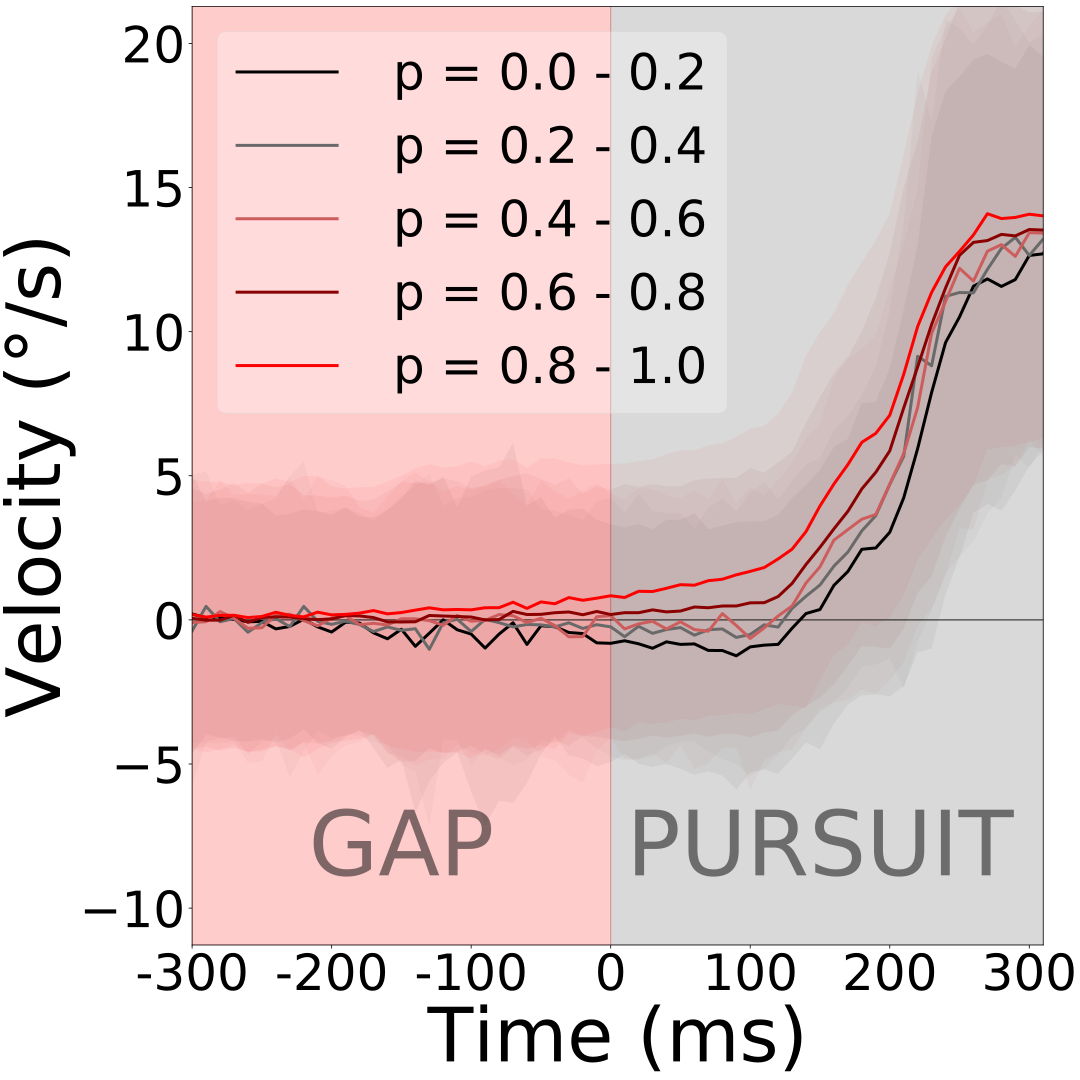
\includegraphics[width=0.33\linewidth]{1_B_Trace_moyenne}};
%%\draw [anchor=north west] (0.000\linewidth, .62\linewidth) node {$\mathsf{(A)}$};
%%\draw [anchor=north west] (0.505\linewidth, .62\linewidth) node {$\mathsf{(B)}$};
%\end{tikzpicture}
%}
%\caption{
%%\emph{Anticipatory SPEM (aSPEM): experimental design and results.}
%%\textbf{(A)}~TODO: MOVE THIS PART IN THE MAIN TEXT:
%\emph{\AM{I GUESS THIS FIGURE WILL BE ELIMINATED...?} Behavioral experiments: anticipatory Smooth Pursuit Eye Movements}
%% TODO : dans notre plot on a des range de valeurs pour p :-/ -> C'EST PARCE QUE LE PLOT REPRESENTE DEJA LA VITESSE MOYENNE OBTENUE DANS LA TACHE AVEC SWITCHES!
%%\textbf{(B)}~
%We first replicated the results of~\citet{Montagnini2010},
%in which human observers were presented with several $500$ trials blocks of horizontal target motion with a block-dependent direction probability bias, and they were asked to track the target with their gaze.
%An important difference with that study is that their experiment was made of several blocks of target motion with a block-dependent direction probability bias selected among a few predetermined values, whereas in the present study $p$ can change in each different block as a random number between $0$ and $1$.
%Horizontal eye velocity traces
%averaged, over rightward trials and all observers, for five different intervals of the direction bias.
%These traces are aligned to the onset of the moving dot (the $0$ on the $x-axis$).
%Saccades were removed using a thresholding method~(see~\seeApp{em}) and
%the shaded area around the traces represent one standard deviation over all velocity samples.
%In the unbiased or weakly biased condition ($0.4\leq p\leq 0.6 $), one can distinguish
%a visually-driven component (after a latency of $\approx 100~\ms$)
%which corresponds to the standard Smooth Pursuit Eye Movement (SPEM) initiation.
%When introducing a bias in the direction,
%the average eye velocity progressively ramps
%in the direction of the expected velocity, starting during the GAP phase and well before the visually-driven component:
%This phase is the anticipatory SPEM (aSPEM).
%As previously reported~\citep{Montagnini2010, SantosKowler2017,Damasse18},
%the slope of this ramp correlates with the strength of the bias.
%In this study, we extended this experiment in three aspects.
%First, we used probability biases in a continuous space,
%as drawn from a prior distribution for the values of $p$.
%Second, we generated the random sequence of trials
%by concatenating random-length blocks (see \seeFig{results_psycho}),
%to avoid potential confounds related to the previously used blocked-design.
%}
%\label{fig:introB}
%\end{figure}
%
%I show here a typical velocity traces for one participant / 2 trials
%
%- x-axis is time in milliseconds aligned on target onset,
%and we show respectively from left to right the fixation in gray,
%the GAP in pink (300\ms) and the run in light gray.
%
%- y-axis is the velocity as computed as the gradient of position.
%Remark that the eyelink provides with the periods of saccades or
% blinks that we removed from the signal. it is quite noisy and
% to complement existing signal processing methods,
% Chloe implemented a robust
%
%- fitting method which allows to extract some key components of
%the velocity traces: maximum speed, latency, temporal inertia ($\tau$)
% and most interestingly acceleration before motion onset.
% We cross-validated that this method was giving similar results
% to other classical methods but in a more robust fashion/
%
%While being sensible to recording errors, this allows us to extract the
% anticipatory component of SPEMs and..

%%%%%%%%%%%%%%%%%%%%%%%%%%%%%%%%
\subsection{Appendix : leaky integrator}
\label{app:leaky}
Given a series of observations $\{x_0^i\}_{0\leq i \leq t}$
with $\forall i, x_0^i \in \{0, 1 \}$, we defined

\eqs{
\hat{x}_1^{t} &= (1-1/\tau)^{t+1} \cdot \hat{x}_1^{t=0} + 1/\tau \cdot \sum_{0\leq i \leq t} (1 - 1/\tau)^{i} \cdot x_0^{t-i}\\
			  &= (1-h)^{t+1} \cdot \hat{x}_1^{t=0} + h \cdot \sum_{0\leq i \leq t} (1 - h)^{i} \cdot x_0^{t-i}
}
%is true for $t=1$: by definition $\hat{x}_1^{0}=x_0^0$ and
%\eq{
%\hat{x}_1^{1} = (1 - \rho) \cdot \hat{x}_1^{0} + \rho \cdot x_0^1
%}
If we write it for trial $t-1$, we have

\eqs{
\hat{x}_1^{t-1}	&= (1-h)^{t} \cdot \hat{x}_1^{t=0} + h \cdot \sum_{0\leq i \leq t-1} (1 - h)^{i} \cdot x_0^{t-1-i} \\
                &= (1-h)^{t} \cdot \hat{x}_1^{t=0} + h \cdot \sum_{1\leq j \leq t} (1 - h)^{j-1} \cdot x_0^{t-j} \\ % j = i+1
(1 - h) \cdot \hat{x}_1^{t-1} &= (1-h)^{t+1} \cdot \hat{x}_1^{t=0} +  h \cdot \sum_{1\leq i \leq t} (1 - h)^{i} \cdot x_0^{t-i}
                }
It follows that the integrative formula above becomes an iterative relation:

\eqs{
\hat{x}_1^{t}	&= (1-h)^{t+1} \cdot \hat{x}_1^{t=0} + h \cdot \sum_{0\leq i \leq t} (1 - 1/\tau)^{i} \cdot x_0^{t-i} \\
				&= (1-h)^{t+1} \cdot \hat{x}_1^{t=0} + h \cdot x_0^{t} + h \cdot \sum_{1\leq i \leq t} (1 - h)^{i} \cdot x_0^{t-i} \\
				&= h \cdot x_0^{t} + (1 - h) \cdot \hat{x}_1^{t-1} \\
}
such that finally

\eq{
\hat{x}_1^{t} = (1 - h) \cdot \hat{x}_1^{t-1} + h \cdot x_0^t
}
As a result, the definitions in~\seeEq{leaky} and~\seeEq{leaky2} are equivalent.


%%%%%%%%%%%%%%%%%%%%%%%%%%%%%%%%
\subsection{The Bernoulli, binomial and Beta distributions}
\label{app:beta}

Let us define some basic concepts. A Bernoulli trial is the outcome of a binary random variable $x$ knowing a probability bias $\mu$ (with $0 \geq \mu \geq 1$) and can be formalized as:

\eq{
Pr(x | \mu) = \mu^x \cdot (1-\mu)^{1-x}
}

The binomial distribution is defined as the probability that the sum $X$ of $\nu$ independent Bernoulli trials is $k$:

\eq{
\Pr(k;\nu,\mu) = \Pr(X = k) = {\nu\choose k} \cdot \mu^k \cdot (1-\mu)^{\nu-k}
}

Knowing such a model for $X$, it can be of interest to find an estimate of the parameter of the Bernoulli trial, that is of the probability bias $\mu$. This distribution function is called the conjugate of the binomial distribution which is the Beta-distribution. For example, the beta distribution can be used in Bayesian analysis to describe initial knowledge concerning probability of success such as the probability that a product will successfully complete a stress test. The beta distribution is a suitable model for the random behavior of percentages and proportions.

It is usually defined using shape parameters $\alpha$ and $\beta$:

\eq{
Pr(p | \alpha, \beta ) = \frac{1}{B(\alpha, \beta)} \cdot p^{\alpha -1} \cdot (1-p)^{\beta - 1}
}
Note that here, the variable is the probability bias $p$. The normalization constant $B(\alpha, \beta)$ is given by the beta function. By definition:

\eqs{
        \alpha &= \mu \cdot \nu \\
        \beta  &= (1-\mu) \cdot \nu
    }
Inversely, $\alpha + \beta = \nu$ and $\mu = \frac{\alpha}{\alpha +\beta} = 1- \frac{\beta}{\alpha + \beta}$


%%%%%%%%%%%%%%%%%%%%%%%%%%%%%%%%
\subsection{Appendix 2: BBCP algorithm}
\label{app:bcp}

To summarize, the algorithm that we presented is an implementation of the  ``Bayesian Online Changepoint Detection'' by~\citet{AdamsMackay2007}
extended for the class of binary inputs. Using the definition of the run-length~\seeSec{Binary_Bayesian_change_point}, the flow-chart of the algorithm is:

\begin{enumerate}
	\item Initialize
	\begin{itemize}
		\item    $P(r_0>0)= 0$ or $P(r_0=0)=1$ and
		\item    $\mu^{(0)}_0 = \mu_{prior}$ and $\nu^{(0)}_0 = \nu_{prior}$
	\end{itemize}

	\item     Observe New Datum $x_0^t \in \{ 0, 1 \}$,

	\begin{enumerate}

		\item    Evaluate Predictive Probability $\pi^{(r)}_{t} = P(x_0^t |\mu^{(r)}_t,\nu^{(r)}_t)$.
	    \item    Calculate Growth Probabilities $P(r_t=r_{t-1}+1, x_{0:t}) = P(r_{t-1}, x_{0:t-1}) \pi^{(r)}_t (1-h)$,
	    \item    Calculate Changepoint Probabilities $P(r_t=0, x_{0:t})= \sum_{r_{t-1}} P(r_{t-1}, x_{0:t-1}) \pi^{(r)}_t \cdot h$,
	    \item    Calculate Evidence $P(x_{0:t}) = \sum_{r_{t-1}} P (r_t, x_{0:t})$,
	    \item    Determine run-length Distribution $P (r_t | x_{0:t}) = P (r_t, x_{0:t})/P (x_{0:t}) $.
	\end{enumerate}

	\item     Update sufficient statistics
		\begin{itemize}
			\item  at a switch  $\mu^{(0)}_{t+1} = \mu_{prior}$, $\nu^{(0)}_{t+1} = \nu_{prior}$,
			\item  else, $\nu^{(r+1)}_{t+1} = \nu^{(r)}_{t} + 1$ and $\nu^{(r+1)}_{t+1} \cdot \mu^{(r+1)}_{t+1} = \nu^{(r)}_{t} \cdot \mu^{(r)}_{t} + x_0^t$.
		\end{itemize}
	\item     Return to step $2$.
\end{enumerate}


In the following, we  detail some intermediate steps and highlight some key differences with their implementation. We also provide a python implementation of the algorithm, which is available at \url{https://github.com/laurentperrinet/Bayesianchangepoint}.

\subsubsection{Initialization}
%to represent our belief at trial $t$
%or to determine the pdf for $x_1^t$ as a mixture of Beta distributions:
%\eqa{
%\hat{x}_1^{t} = \sum_{r^{t}} Pr(x_1^t | r^{t}, x_0^{0:t}) \cdot Pr(r^{t} | x_0^{0:t})
%}

% in Python.
%
%
%* adapted from https://github.com/JackKelly/Bayesianchangepoint by Jack Kelly (2013)

%
%* This code is based on the [MATLAB implementation](http://www.inference.phy.cam.ac.uk/rpa23/changepoint.php) provided by Ryan Adam. Was available at http://hips.seas.harvard.edu/content/Bayesian-online-changepoint-detection
%
% * full code @ https://github.com/laurentperrinet/bayesianchangepoint are available .



Note that the prior distribution is itself a Beta distribution:
$\Pp\propto B(p; \mu_{prior}, \nu_{prior})$.
It will by symmetry be unbiased: $\mu_{prior}=.5$.
Concerning the shape, it can be for instance
the uniform distribution $\Uu$ on $ [ 0, 1 ] $, that is $\nu_{prior}=2$ or
Jeffrey's prior $\Jj$, that is $\nu_{prior}=1$.
We chose the latter for the generation of trials
as the uniform distribution would yield more samples around $.5$.
Qualitatively, this would result in more difficult task in discriminating a probability bias from another.
Jeffrey's prior was more adapted to that task.
%Wikipedia: Beta(1/2, 1/2): The arcsine distribution probability density was proposed by Harold Jeffreys to represent uncertainty for a Bernoulli or a binomial distribution in Bayesian inference, and is now commonly referred to as Jeffreys prior: p−1/2(1 − p)−1/2. This distribution also appears in several random walk fundamental theorems


\subsubsection{Prediction: run-length distribution}

The steps to achieve the update rule are:

 \eqs{
%\hat{x}_1^{t} =
Pr(x_0^t | x_0^{0:t-1}) &= \sum_{r^{t}} Pr(x_0^t | r^{t}, x_0^{0:t-1}) \cdot  \beta^{(r)}_t \\
Pr(x_0^t | x_0^{0:t-1}) &= \sum_{r^{t}} Pr(x_0^t | r^{t}, x_0^{0:t-1}) \cdot  Pr(r^{t} | x_0^{0:t-1})\\
\text{with} \quad Pr(r^{t} | x_0^{0:t-1}) &\propto \sum_{r^{t-1}}  Pr(r^t | r^{t-1}) \cdot  Pr(x_0^t | r^{t-1}, x_0^{0:t-1}) \cdot  Pr(r^{t-1} | x_0^{0:t-2})
}
Finally we obtain~\seeEq{pred_node}:
\eq{
\beta^{(r)}_t \propto \sum_{r^{t-1}}  Pr(r^t | r^{t-1}) \cdot  Pr(x_0^t | r^{t-1}, x_0^{0:t-1}) \cdot  \beta^{(r)}_{t-1}
}


\subsubsection{Prediction: sufficient statistics}

The recursive formulation in~\seeEq{update_nu} and~\seeEq{update_mu} comes from the expression

 \eq{
\nu^{(r)}_{t} \cdot \mu^{(r)}_{t} = \sum_{i=t-r-1}^{t-1} x_0^i % + 2 - \nu_{prior}
}
and therefore

\eqs{
\nu^{(r+1)}_{t+1} \cdot \mu^{(r+1)}_{t+1} 	&= \sum_{i=t+1-r-1-1}^{t+1-1} x_0^i  \\% + 2 - \nu_{prior} \\
											&=  \sum_{i=t-r-1}^{t} x_0^i  \\% + 2 - \nu_{prior}\\
											&= \nu^{(r)}_{t} \cdot  \mu^{(r)}_{t} +  x_0^t
}

%\subsubsection{Readout}
%\label{app:readout}
%
%Perform Prediction $P (x_0^{t+1} | x_{0:t}) = P (x_0^{t+1}|x_{0:t} , r_t) P (r_t|x_{0:t})$,
%
%Can we get  $P (x_2^{t+1} | x_{0:t}) $ ? would be nice to see the inferrence of surprise / would fit with pupil size...

\subsubsection{Quantitative evaluation}

To quantitatively evaluate our results with respect to another probability bias, we computed in~\seeEq{KL} the cost as the Kullback-Leibler divergence  $\KL{\hat p}{p}$ between samples $\hat p$ and model $p$ under the hypothesis of a Bernoulli trial:

\begin{equation}
\KL{\hat p}{p} = \hat{p} \cdot\log\pa{\frac{\hat p}{p}} + (1-\hat p)\cdot \log\pa{\frac{1-\hat p}{1-p}}.
\end{equation}


%%%%%%%%%%%%%%%%%%%%%%%%%%%%%%%%
\subsection{Appendix: likelihood function}
\label{app:likelihood}
%\seeApp{likelihood}
% TODO : check http://www.princeton.edu/~rcw2/papers/WilsonEtAl_PLOSCompBiol2013.pdf and Bernoulli case + evaluation
%cf p33 de 2018-02-12 journal club Bayesian changepoint chloe.pdf
%cf p52 de 2017-10-05 chloe inverting the process rem jb.pdf


We want to compute $\Ll(r | o) = Pr(o | p, r)$ where $o \in \{ 0, 1 \}$ such that we can evaluate Predictive Probability $\pi_{0:t} = P(x_0^t  |\mu^{(r)}_t,\nu^{(r)}_t)$ in the algorithm above with $\mu^{(r)}_t$ and $\nu^{(r)}_t$ the sufficient statistics at trial $t$ for node $(r)$.
The likelihood of observing $o=1$ is that of a binomial (conjugate of a Beta distribution) of
	\begin{itemize}
		\item  mean rate of choosing hypothesis $o=1$ equal to $\frac{p\cdot r + o}{r+1}$,
		\item number of choices where  $o=1$ equals to $p\cdot r+1$.
	\end{itemize}
More generally, by observing $o$, the new rate is $p^{'} = \frac{p\cdot r + o}{r+1}$.

\subsubsection{Mathematical derivation}

The likelihood will give the probability of this novel rate given the known parameters and their update (in particular $r^{'}=r+1$):

\eqs{
L(r | o)&={(\frac{p\cdot r + o}{r+1})}^{p\cdot r + o} \cdot (1-\frac{p\cdot r + o}{r+1})^{r + o - (p\cdot r + o)} \\
&= \frac{1}{({r+1})^{r+1}} \cdot {(p\cdot r + o)}^{p\cdot r + o}  \cdot {((1- p)\cdot r + 1- o)}^{(1- p)\cdot r + 1- o} \\
%&= \frac{ (1-o) \cdot {(p\cdot r)}^{p\cdot r}  \cdot {((1- p)\cdot r + 1)}^{(1- p)\cdot r + 1}
%+ o \cdot {(p\cdot r + 1)}^{p\cdot r + 1}  \cdot {((1- p)\cdot r)}^{(1- p)\cdot r}
% }{
% {(p\cdot r + 1)}^{p\cdot r + 1}  \cdot {((1- p)\cdot r )}^{(1- p)\cdot r }  +
%  {(p\cdot r )}^{p\cdot r }  \cdot {((1- p)\cdot r + 1)}^{(1- p)\cdot r + 1}
%}  \\
}
since both likelihood sum to 1, the likelihood of drawing $o$ in the set $\{ 0, 1 \}$   is equal to

%\AM{the change in the argument of $\Ll$}
\eqs{
\Ll(r | o)&=\frac{L(r | o)}{L(r | o=1) + L(r | o=0)}  \\
&= \frac{ {(p\cdot r + o)}^{p\cdot r + o}  \cdot {((1- p)\cdot r + 1- o)}^{(1- p)\cdot r + 1- o} }{
 {(p\cdot r + 1)}^{p\cdot r + 1}  \cdot {((1- p)\cdot r )}^{(1- p)\cdot r }  +
  {(p\cdot r )}^{p\cdot r }  \cdot {((1- p)\cdot r + 1)}^{(1- p)\cdot r + 1}
}  \\
&= \frac{ (1-o) \cdot {(p\cdot r)}^{p\cdot r}  \cdot {((1- p)\cdot r + 1)}^{(1- p)\cdot r + 1}
+ o \cdot {(p\cdot r + 1)}^{p\cdot r + 1}  \cdot {((1- p)\cdot r)}^{(1- p)\cdot r}
 }{
 {(p\cdot r + 1)}^{p\cdot r + 1}  \cdot {((1- p)\cdot r )}^{(1- p)\cdot r }  +
  {(p\cdot r )}^{p\cdot r }  \cdot {((1- p)\cdot r + 1)}^{(1- p)\cdot r + 1}
}
}
This can also be written by isolating the part which depends on $o$ and for a given run-length and knowing sufficient statistics describing the sufficient statistics at each node $r$:

\eql{
\Ll(r | o) = \frac{1}{Z} \cdot {(p \cdot r + o)}^{p \cdot r + o} \cdot {((1- p)\cdot r + 1- o)}^{(1- p)\cdot r + 1- o}
}
with $Z$ such that $\Ll(r | o=1) + \Ll(r | o=0)=1$, that is~\seeEq{likelihood}.

\subsubsection{Python code}

\begin{lstlisting}
def likelihood(o, p, r):
    """
    Knowing $p$ and $r$, the sufficient statistics of the beta distribution $B(\alpha, \beta)$ :
    $$
        alpha = p*r
        beta  = (1-p)*r
    $$
    the likelihood of observing o=1 is that of a binomial of

        - mean rate of choosing hypothesis "o=1" = (p*r + o)/(r+1)
        - number of choices where  "o=1" equals to p*r+1

    since both likelihood sum to 1, the likelihood of drawing o in the set {0, 1}
    is equal to

    """
    def L(o, p, r):
        P =  (1-o) * ( 1. - 1 / (p * r + 1) )**(p*r) * ((1-p) * r + 1)
        P +=  o * ( 1. - 1 / ((1-p) * r + 1) )**((1-p)*r) * (p * r + 1)
        return  P

    L_yes = L(o, p, r)
    L_no = L(1-o, p, r)
    return L_yes / (L_yes + L_no)

\end{lstlisting}

See the code \href{https://github.com/laurentperrinet/bayesianchangepoint/blob/master/bayesianchangepoint/bcp.py#L65}{online}.
\subsubsection{Properties}
This function has some properties, notably symmetries:
	\begin{itemize}
		\item for certain outcomes, $\forall r >0$, $\Ll(o|p=0, r)=1-o$ and $\Ll(o|p=1, r)=o$,
		\item if $r=0$, the likelihood is uniform $\Ll(o)=1/2$,
		\item $Pr(o | p, r)=Pr(1-o | 1-p, r)$.
	\end{itemize}

\noindent Note also that as $r$ grows, the likelihood gets sharper.

% TODO : put figure from https://github.com/laurentperrinet/Bayesianchangepoint/blob/master/notebooks/test_tracebase.ipynb

%%%%%%%%%%%%%%%%%%%%%%%%%%%%%%%%
%%%%%%%%%%%%%%%%%%%%%%%%%%%%%%%%
%\subsection{Appendix 4: Supplementary psychophysical results}
%\label{app:results_psycho}
%%\seeApp{results_psycho}
%%%%%%%%%%%%%%%%%%%%%%%%%%%%%%%%
%%%%%%%%%%%%%%%%%%%%%%%%%%%%%%%%
%%%%%%%%%%%%%%%%%%%%%%%%%%%%%%%%
\end{document}%
